\documentclass[11pt,a4paper]{report}
%\usepackage{fullpage}
\usepackage{graphics}
\usepackage{setspace}
\usepackage{caption}
\usepackage{subcaption}
\usepackage{hyperref}
\usepackage{tikz}
\usepackage{pgfgantt}
\usepackage{lscape}
\usepackage{appendix}
\usepackage{fancyhdr}
\usepackage[utf8]{inputenc}
\usepackage[nottoc,notlof,notlot,numbib]{tocbibind}
\usepackage{pgfplots}
\usepackage[backend=bibtex,style=authoryear,natbib=true]{biblatex}
\pgfplotsset{compat=newest}

% tweak for bar graph legend
\pgfplotsset{compat=1.11,
  /pgfplots/ybar legend/.style={
  /pgfplots/legend image code/.code={%
     \draw[##1,/tikz/.cd,yshift=-0.25em]
      (0cm,0cm) rectangle (0.8em,0.8em);},
 },
  /pgfplots/xbar legend/.style={
  /pgfplots/legend image code/.code={%
     \draw[##1,/tikz/.cd,yshift=-0.25em]
      (0cm,0cm) rectangle (0.8em,0.8em);},
 },
}
\usetikzlibrary{shapes,arrows}
\onehalfspacing
\hypersetup{
  colorlinks=false,
  pdfborder={0 0 0},
}
\setcounter{tocdepth}{1}

% set up page header/footer
\pagestyle{fancy}
\renewcommand{\chaptermark}[1]{\markboth{#1}{}}
\renewcommand{\headsep}{25pt}
\fancyhead[LE,RO]{\thepage}
\fancyhead[LO]{\scshape\MakeTextLowercase{\leftmark}}
\fancyhead[RE]{\scshape\MakeTextLowercase{\chaptername~\thechapter}}
\fancyfoot{}

\bibliography{refs}

\begin{document}

\begin{titlepage}
  \vspace*{\fill}
  \begin{center}
    {\Huge Semantic Audio Tools for Radio Production}\\[1cm]
    {\Large Christopher M. Baume}\\[1cm]
    {\large Submitted for the degree of\\Doctor of Philosophy\\from the\\
      University of Surrey}\\[1cm]
    \begin{center}
      
\includegraphics[width=6cm]{figs/surrey-logo.png}\\[1cm]
    \end{center}
    {\small Centre for Vision, Speech and Signal Processing,\\
      Faculty of Engineering and Physical Sciences,\\
      University of Surrey,\\
      Guildford, Surrey GU2 7XH, U.K.}
  \end{center}
  \vspace*{\fill}
\end{titlepage}

\chapter*{Abstract}

Radio production is a creative pursuit that uses sound to inform, educate and entertain an audience. Radio producers
use audio editing tools to visually select, re-arrange and assemble sound recordings into programmes. However, current
tools represent audio using waveform visualizations that display limited information about the sound.

Semantic audio analysis can be used to extract useful information from audio recordings, including when people are
speaking and what they are saying. This thesis investigates how such information can be applied to create
semantic audio tools that improve the radio production process.

An initial ethnographic study of radio production at the BBC reveals that producers use textual representations and
paper transcripts to interact with audio, and waveforms to edit programmes. Based on these findings, three
methods for improving radio production are developed and evaluated, which form the primary contribution of this thesis.

Audio visualizations can be enhanced by mapping semantic audio features to colour, but this approach had not been
formally tested. We show that with an enhanced audio waveform, a typical radio production task can be completed faster,
with less effort and with greater accuracy than a normal waveform.

Speech recordings can be represented and edited using transcripts, but this approach had not been formally evaluated
for radio production. By developing and testing a semantic speech editor, we show that automatically-generated
transcripts can be used to semantically edit speech in a professional radio production context, and identify
requirements for annotation, collaboration, portability and listening.

Finally, we present a novel approach for editing audio on paper that combines semantic speech editing with a digital
pen interface. Through a user study with radio producers, we compare the relative benefits of semantic speech editing
using paper and screen interfaces. We find that paper is better for simple edits of familiar audio with accurate
transcripts.



% !TeX root = main.tex
\chapter*{Acknowledgements}

My foremost thanks go to my supervisor, Prof. Mark Plumbley, for his ethusism, encouragment, wisdom and guidance over
the years. Huge thanks also to my co-supervisors: Dr. Nick Bryan-Kinns, Dr. Janko \'{C}ali\'{c} and Prof.  David
Frohlich, for their invaluable suggestions, feedback and advice, and for helping me navigate an unfamiliar field of
research.

I have been extremely privileged to have been able to undertake this research as part of my employment at the BBC.  My
heartfelt thanks go out to Prof. Graham Thomas, Dr. Frank Melchior, Chris Pike and Samantha Chadwick for giving me this
rare opportunity, and for their steadfast support throughout the process.  Many thanks to my colleagues in the BBC R\&D
Audio Team for their patience, support and help with proofreading, but also for being brilliant people to work with.

This work was only made possible through the involvement of colleagues from BBC Radio, who volunteered their time
despite their demanding workload. My sincere thanks go to all of the radio producers who took the time to participate
in the user studies and contribute to the design of the interfaces. Thanks also to Deborah Cohen, Hugh Levinson and
John Goudie for allowing me access to their teams, and to Jonathan Glover his advocacy and encouragement.

Thanks to Matt Haynes and Matt Shotton from BBC R\&D, whose software formed part of the semantic speech editor, and to
Liam Bowes, Carl Garner and Richard Sargeant from Anoto for their support in the development of the digital pen
interface. 

Finally, I'd personally like to thank my wife, Nancy, for her love, encouragement, patience and belief in me throughout
this process. I couldn't have done it without you.

\vfill
\noindent
The work in this thesis was fully funded by the British Broadcasting Corporation as part of the BBC Audio Research
Partnership.


{\singlespacing
\tableofcontents
}

\listoffigures

\listoftables

\chapter*{List of abbreviations}

%\begin{center}
\begin{tabular}{l l}
DAW & Digital Audio Workstation \\
EDL & Edit Decision List \\
TLA & Three Letter Acronym
\end{tabular}
%\end{center}


% !TeX root = main.tex
\chapter{Introduction}\label{chpt:intro}

Want to improve interface for professionally working with audio content

Semantic audio analysis can extract useful information, but how can this best be used?

Tasks are creative, so can't easily be automated

Humans and machines working to their strengths

\section{Motivation}\label{sec:intro/motivation}
Ever since the first digital audio workstations were introduced in the early
1990s, the audio waveform has been the primary method of navigating audio
content. The waveform works well for finding amplitude-related events such as
silences and peaks, but is very poor at conveying much more about the sound of
the content. Additionally, the waveform doesn't scale well as demonstrated by
the `Soundcloud sausage' (see Figure~\ref{fig:soundcloud}), where even at
reasonable zoom levels, no useful information is presented.  A popular
alternative to the waveform is the spectrogram, which displays detailed
information about the frequency content. However, these can be very difficult
to interpret and require training and practice to be of use.

\begin{figure}[ht]
  \centering
  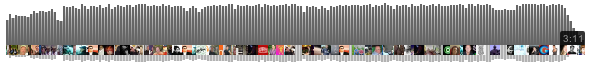
\includegraphics[width=0.6\textwidth]{figs/soundcloud.png}
  \caption{An example of a waveform visualization on the online music sharing
    service Soundcloud}
  \label{fig:soundcloud}
\end{figure}

\section{Aim}\label{sec:intro/aim}
This projects aims to develop better visualization for helping radio producers
navigate audio content by initially targeting a number of common tasks. Audio
features will be identified or developed which are able to capture the
information required for the task. Methods of mapping these features to an
image will be created so that the information is presented in a perceptible way
which requires little or no training. 

\section{Thesis structure}\label{sec:intro/structure}

\paragraph{Chapter \ref{chp:background}} reviews existing work and literature
from three areas that will feed into the project -- feature extraction,
visualization and cross-modal links.

\paragraph{Chapter \ref{chp:colourised}} details the process and results of an
initial online study which looked at how the waveform performs in a common
production tasks, and whether it can be improved.

\paragraph{Chapter \ref{chp:ethno}} provides a comprehensive overview of
the radio production process at the BBC, which will help put this research into
context.

\paragraph{Chapter \ref{chp:screen-based}} investigates how a screen-based semantic audio editing interface affects the
production process.

\paragraph{Chapter \ref{chp:paper-based}} investigates how a paper-based semantic audio editing interface compares to
the screen-based approach and normal paper.

\paragraph{Chapter \ref{chp:conclusions}} concludes the thesis and considers the prospects for future research.

\section{Contributions}\label{sec:intro/contributions}

The principal contributions of this thesis are:
\begin{itemize}
  \item Chapter~\ref{chp:colourised}: 
  \item Chapter~\ref{chp:ethno}: 
  \item Chapter~\ref{chp:screen-based}: 
  \item Chapter~\ref{chp:paper-based}: a novel system for editing speech-based audio using digital pens on printed transcripts
  \item Appendix~\ref{sec:discourse}: an open-source semantic audio editing system
  \item Appendix~\ref{sec:vampeyer}: an open-source audio visualisation plugin framework
  \item Appendix~\ref{sec:beatmap}: an open-source library for rendering tiled audio visualisation in web browsers
\end{itemize}

%In addition, this work has produced the following technological developments:
%
%\begin{itemize}
%  \item `Discourse' -- a screen-based semantic audio editing system, available as open source
%    software\footnote{\url{https://github.com/bbc/discourse}}. See Section~\ref{sec:discourse}.
%  \item A digital pen system for editing audio using printed transcripts.
%  \item `Vampeyer' -- an audio visualisation plugin framework, available as open source
%    software\footnote{\url{https://github.com/bbc/vampeyer}}. See Section~\ref{sec:vampeyer}.
%  \item `Beatmap' -- a Javascript user interface element for audio visualisation based on tiled bitmaps, available as
%    open source software\footnote{\url{https://github.com/bbc/beatmap}}. See Section~\ref{sec:beatmap}.
%\end{itemize}

\section{Associated publications}\label{sec:intro/publications}

Portions of the work detailed in this thesis have been presented in the following publications:

\begin{itemize}
  \item Chapter~\ref{chp:ethno}: The results of this work were published and presented at the 138th Audio Engineering Society Conference in
    Warsaw, Poland \citep{Baume2015}
\end{itemize}


% !TeX root = main.tex
\chapter{Background}\label{chp:background}

Audio is an electronic representation of sound which stores pressure waves as an electrical signal.
Sound is by its very nature time-variant, which makes it both fascinating and challenging.
This temporal property makes it impossible to `freeze' sound, or to experience it in an instant. Listening is a
time-consuming activity, because sound must be consumed over time.

%There have been many attempts to create tools that
%compress the time needed to listen, which are detailed in Section~\ref{sec:background-auditory}.
%These tools still require the user to invest time in the task.

% Sound is linear - has a beginning and an end, constrained by the arrow of time
% Cannot be searched or skimmed
% Sound is one-dimensional
% We never stop listening
% Huge range of frequencies and pressure levels

This also poses a challenge when designed interfaces for interacting with audio content. Dealing with large amounts of
audio in a reasonable time requires the use of tools that can shorten the time needed to complete tasks such as
navigation.

In this chapter, we consider the various approaches that have been used to help users navigate audio content.
A number of approaches have been excluded as they specifically target music content (e.g. chromagrams and music
transcripts).

In section \ref{sec:visualization} we introduce the foundations of audio visualisation and discuss the two most common
visualisation techniques. In section \ref{sec:semantic}, we show how these visualisations can be improved by combining
them with semantic audio analysis techniques. Finally in section \ref{sec:auditory}, we look at non-visual interfaces
to audio, including auditory and haptic techniques.

\section{Radio production}\label{sec:background-radio}

The process and tools for radio production are well-understood and books have been written about it
\citep{McLeish2015,Hausman2012}.

\section{Audio visualization}\label{sec:background-visualization}

\citet{Arons1997} found that most humans cannot comprehend speech which it is played faster than twice real-time. This
means that there is a limit on the improvement that can be gained with using continuous audio playback.

Vision is very different medium that varies not only over time, but over space. When you remove the element of time,
you are left with an image that can be experienced instantanously, searched and skimmed.
Human vision can be used to process complex scenes at a glance
%Anderson 2009; Belopolsky et al. 2008; Goldstein 2010
For this reason, visualisation is a good way to interact with time-variant information.
\citet{Aigner2011} contains a collection of examples of how this can be done.

Visual systems can be used to complement audio interfaces, as they are able to address the key challenges of sound.

In modern society, screens for displaying visual content are widely available.

To be able to represent audio visually, we must map auditory properties to visual properties. We could select these 
to have a general mapping, which attempts to cover all use cases, or a selective mapping that targets a particular use
case.

When attempting to link sound and vision, it is desirable to create a mapping that is coherent and makes sense to the
user. The ultimate goal would be to create an audio visualisation that ``look likes it sounds'', as this would
allow users to comprehend the sound without having to listen to it.

%In a world of `big data', data visualization is becoming an increasing popular
%subject. Visualization techniques have been applied to audio content for a
%variety of applications including accessibility \citep{Ho-Ching2003}, browsing
%large databases \citep{FontCorbera2010}, browsing small databases \citep{Yoo2011}
%and musical training \citep{Ferguson2005} amonst others.

%The development of good visualizations lies somewhere between science and art.
%Tufte's seminal work on good practice \citep{Tufte2001} gives solid guidance on
%creating elegent and unbiased visuals, and Wolfe and Horowitz \citep{Wolfe2004}
%tell us which properties of vision are most critical for visual search.
%However, putting these together in the context of audio requires a certain
%amount of creativity.

%This project focusses on `visualization of time-oriented data', a good overview
%of which can be found in a Springer book of the same name \citep{Aigner2011}.
%The rest of this section will look at examples of time-oriented visualization
%of audio, grouped by the most common visualization techniques.

\subsubsection{Crossmodality}
Crossmodal perception is a term used to describe interaction between the different senses. This phenomenon has been
studied over many years by psychologists, who have discovered perceptual mappings between auditory and visual stimuli.

The ``bouba/kiki effect'' is a demonstration of cross-model mapping between vision and audition, originally discovered
in an experiment run by psychologist \citet{Koehler1929}. In the experiment, participants are shown two abstract shapes
and are asked to assign the name `bouba' to one of them, and `kiki' to the other\footnote{K\"ohler used the words
  `baluma' and `takete' in the original experiment, but the result was the same.}. To try out the experiment for
yourself, without reading ahead look at the shapes in Figure~\ref{fig:boubakiki} and see which shape you think best
fits the name `bouba' and which best fits `kiki'.

\begin{figure}[ht]
\centering
\begin{subfigure}{.5\textwidth}
  \centering
  
\includegraphics[width=0.7\linewidth]{figs/kiki.png}
  %\caption{Kiki}
  \label{fig:kiki}
\end{subfigure}%
\begin{subfigure}{.5\textwidth}
  \centering
  
\includegraphics[width=0.7\linewidth]{figs/bouba.png}
  %\caption{Bouba}
  \label{fig:bouba}
\end{subfigure}
  \caption{Demonstration of the ``bouba/kiki effect'' \citep{Ramachandran2001}}
  \label{fig:boubakiki}
\end{figure}

K\"{o}hler found that the vast majority of participants chose to name the sharp, pointy shape `kiki' and the curvy,
rounded shape `bouba'. \citet{Ramachandran2001} found that that this effect holds for 95--98\% of the population. This
is an example of just one audio-visual mapping that is common amongst the population.

%\citep{Hubbard1996}

%These audio-visual associations are not just higher-level constructs that our
%concious brain creates, they affect the brain at the very lowest level even
%with only brief exposure to bimodal stimuli. Zangenehpour et. al.
%\citep{Zangenehpour2010} used a PET-CT scanner to measure blood flow in the
%brain during exposure to audio and visual stimuli. ``When presented with only
%the auditory or visual components of the bimodal stimuli, na\"{i}ve subjects
%showed only modality-specific cortical activation, as expected.  However,
%subjects who had previously been exposed to the audiovisual stimuli showed
%increased cerebral blood flow in the primary visual cortex when presented with
%sounds alone.''

\citet{Spence2011} reviewed a wide range of psychology experiments that attempt to find the inherint cross-modal links
in the human brain, including audio-visual mapping.  There are two common types of test methods used to discover these
links -- `speeded' and `unspeeded'.  In `speeded' tests, participants are tasked with classifying an audio/visual
stimulus and their reaction time is measured. When the auditory and visual stimuli are `congruent' (perceived to be
similar), then their reaction times are quicker. In `unspeeded' tests, visual and audio stimuli are presented very
quickly, one after the other, and participants are asked to select which stimulus came second. When the stimuli are
congruent, participants find it more difficult to work out the order of presentation.
Through his literature review, \citet{Spence2011} found there to be strong evidence for six audio-visual mappings,
which he grouped into three categories, shown in Table~\ref{tab:crossmodal}.

\begin{table}
\centering
\begin{tabular}{|l|l|l|}
\hline
\textbf{Type} & \textbf{Link} & \textbf{Direction} \\ \hline
Structural    & Loudness/brightness  & louder=brighter \\ \hline
\multirow{3}{*}{Statistical} & Pitch/elevation & higher=higher \\ \cline{2-3}
              & Pitch/size & higher=smaller \\ \cline{2-3}
              & Loudness/size & louder=bigger \\ \hline
\multirow{2}{*}{Semantic} & Pitch/elevation & higher=higher \\ \cline{2-3}
              & Pitch/spatial frequency & higher=higher \\ \hline
\end{tabular}
\caption{Audio-visual mappings supported by strong evidence \citep{Spence2011}}
\label{tab:crossmodal}
\end{table}

\citet{Tsiros2014} used a different approach to measure audio-visual crossmodality by using audio visualization
techniques.  Three audio recordings were used -- a violin, recording of wind noise and impact sound event. For each,
images were manually created which used different combinations of audio-visual mappings (e.g. dissonance $\to$ texture
granularity). Participants were played an audio clip and shown an image and were asked whether they are similar or not,
and to what degree (on a scale of 0--100).  The experiment confirmed previous results which found strong links between
size/loudness and pitch/elevation, and weaker links between colour/pitch, granularity/dissonance, and colour
complexity/dissonance.

Additional work from \citet{Marks2003}.

%Vision and audition are physiologically separate, but idential in many respects
%\citep{Tsiros2013}.

In this section, we have seen that the temporal constraints of audio can be overcome by using the spatial properties of
vision. These mappings can be designed to be general, or address specific tasks. There are underlying links between
sound and vision that could be exploited to make more perceptually relevant visualisations.

\subsection{Waveforms}

An audio waveform is the graphical representation of an audio signal. It is perhaps the simplest audio visualisation
technique available and arguably the most commonly used.

Audio waveforms have been used to visually representing audio content ever since the first digital audio workstations
started to appear \citep{Massie1985}. Despite their ubiquity, they display very little relevant information and are not
well-suited towards most audio navigation or editing tasks. For instance, it is almost impossible to distinguish
between individual voices with a waveform, even if they sound very different.

% ==== PROS ====

The curve of an audio waveform directly represents the pressure waves of the sound, so the amplitude and frequency of
the sound is mapped to the amplitude and frequency of the plot. This makes it conceptually easy for users to
understand how the audio is represented.

Large curves represent loud sounds, and spatially high frequency curves represent high sound frequencies. These
mappings corrolate with two of the most common cross-modal links (see Table~\ref{tab:crossmodal}).

Waveforms operate in the time domain and can be plotted using a linear function of the audio signal, which makes them
computationally efficient to generate. 

For these reasons, it is the default audio visualisation used in all audio editing software that we have come across.

% ==== CONS ====

In waveforms, frequencies are visible (see Figure~\ref{fig:waveform-zoomin}) at the right scale, but it is hard to work
out which exactly which frequencies are present and in what proportion.

Given a high enough resolution, waveforms can be losslessly be converted back into the original audio signal. In this
sense, they can fully represent the information contained in the audio. However for any practical application, the
time axis of the waveform must be downsampled so that the waveform can be viewed at a reasonable scale (see
Figure~\ref{fig:waveforms}).  This downsampling causes the frequency informaton to be lost, and what remains is the
profile of the audio amplitude.

``Graphically displaying an audio recording as a waveform would generally be inappropriate because, for most users, the
audio signal spectrum offers no information about content'' \citep{Bouamrane2007}.

\citet{Loviscach2011}
proposed an elegant solution to this problem using a technique he calls the `quintessence waveform'. This approach
used extreme pitch shifting to preserve the character of the waveform at different scales (see Figure~\ref{fig:quint}).
Although this approach works well for regular monoaural sounds such as sine waves, it cannot be used for the complex
polyphonic audio used in most real-life applications.

\begin{figure}[p]
\centering
\begin{subfigure}{.5\textwidth}
  \centering
  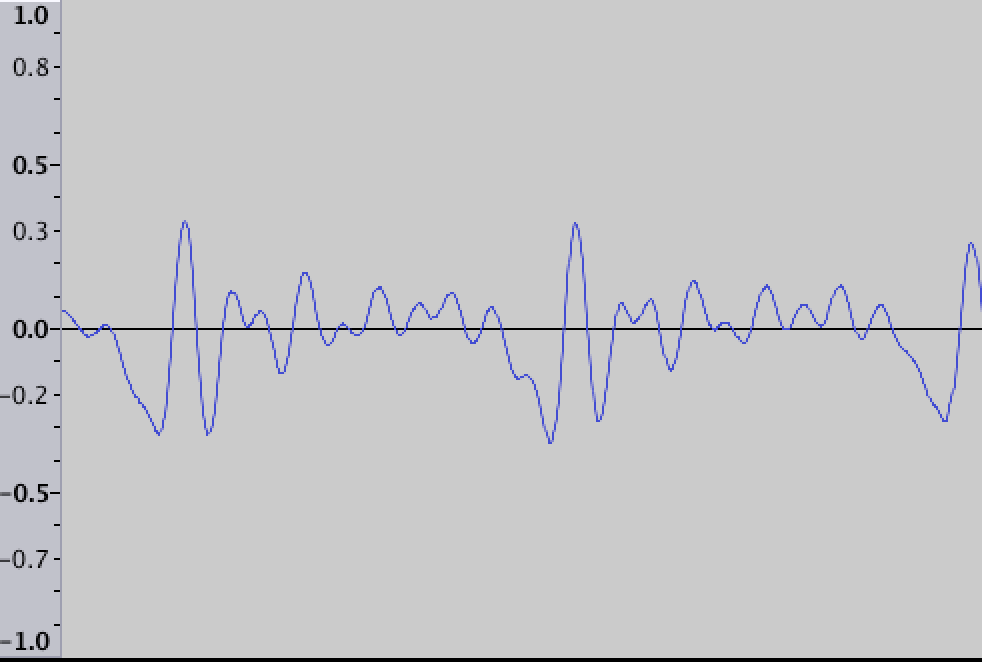
\includegraphics[width=.9\linewidth]{figs/waveform-zoomin.png}
  \caption{When zoomed-in, the frequency information is visible}
  \label{fig:waveform-zoomin}
\end{subfigure}%
\begin{subfigure}{.5\textwidth}
  \centering
  
\includegraphics[width=.9\linewidth]{figs/waveform-zoomout.png}
  \caption{When zoomed-out, the frequency information is lost and only the amplitude profile is visible}
  \label{fig:waveform-zoomout}
\end{subfigure}
\caption{The effect of scaling on waveform frequency information}
\label{fig:waveforms}
\end{figure}

\begin{figure}[p]
  \centering
  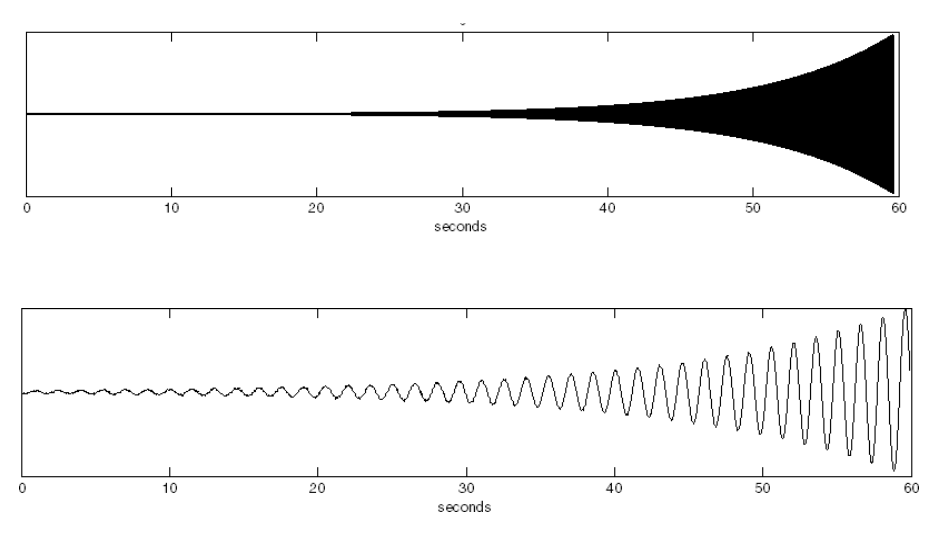
\includegraphics[width=0.95\linewidth]{figs/quint.png}
  \caption{Above: Normal waveform, below: quintessence waveform, source:
  \citep{Loviscach2011}}
  \label{fig:quint}
\end{figure}

\citet{Gohlke2010} proposed a number of ideas for how to improve waveform displays.
%TODO Expand

This amplitude profile can be used to infer some information about the audio content. For example, speech content has
frequent short periods of silence between words, whereas music has few periods of silence. However, in order to be able
to read this information, users must learn what the different profiles of sounds look like.

Many professional engineers and producers have worked with waveforms for most of their career, and have developed the
skills to be able to read waveforms.  However, without frequency content, there is a limit to the amount of information
waveforms can convey.

\subsubsection{User studies}

We searched for studies that considered the performance of waveforms as an interface to audio content. Although X and Y
included waveforms in their studies, the waveforms themselves were not assessed. No studies could be found that
consider the performance of the waveform itself.

\subsection{Spectrograms}
The spectrogram is a visual representation of the spectrum of frequencies in an audio signal over time.  This technique
allows the full frequency content of the audio to be visible to the user. It is a simple mapping that can be easily
understood, and a generic visualisation that can be used for a wide variety of applications.

Unlike waveforms, spectrograms make it easy for the user to see the frequencies that make up the sound, and in what
proportions. When the time axis of spectrograms is rescaled, the frequency information is still visible, so it is much
more robust to scaling than waveforms. This allows a higher density of information at typically-used scales.

The frequency scale in an audio spectrogram is usually presented on a logarithmic or Mel scale to give a better mapping
of frequencies to the perception of pitch. Psuedocolour (see Section~\ref{sec:pseudocolour}) is often used so that the
detail is more visible.

Higher audio frequencies are displayed at the top of the spectrogram, and the energy of the signal is mapped to the
intensity of the colour. Like with waveforms, these corrolate to two of the cross-modal links listed in
Table~\ref{tab:crossmodal}.

Spectrograms are available in most audio editing software, but rarely used by default. As spectrograms are based on a
Fourier analysis, they are more computationally expensive to plot than waveforms, but trivial for modern computers to
generate.

Although spectrograms present the data very clearly, users must still learn how to interpret the information.  
\citet{Zue1986} found that expert users were able to use spectrograms to read the phonemes of speech, but this is
impossible for the average user to achieve.

The spectrogram displays the energy present in each frequency band, however this can make it difficult for the user to
see the overall energy at a given time.

Spectrograms have a wide range of parameters which control how the data is displayed, including window size and 
shape, frequency and energy scaling, min/max values and pseudocolour methods. This means that is a great deal of
inconsistency between spectrogram, which can make it difficult for users to move from one to the other.

Understanding spectrograms requires users to have basic knowledge about how audio is composed of multiple frequencies.
They would also benefit from understanding how frequencies interact, such as harmonics.

%Pros
%X info rich
%X robust to scaling
%X already available
%X simple and generic visualisation
%X computatonally easy

%Cons
%X more computationally expensive than waveforms
%X must learn what different things look like - hard to map frequencies to info
%(doesn't take into account octaves and harmonics)
%X total energy is unclear
%X users must understand that audio is composed of a spectrum of frequencies
%X multiple parameters needed to control visualisation - inconsistent (e.g. window size, window type, 

Spectrograms provide an information-rich and scalable alternative to waveforms, and they are widely available in most
audio editing software. Despite this, waveforms remain a more popular way of interacting with audio. It is unclear as
to why this is.

\subsubsection{User studies}

\citet{Goudeseune2012} used spectrograms as a basis to develop an interface for finding acoustic events.  They filtered
the spectrogram using image processing techniques to create a salience map (see Figure~\ref{fig:timeliner}). This
attempts to dim the background noise to make acoustic events clearer to the user.  Through the use of custom browsing
software called Timeliner, the system was tested by recording how quickly users could find sound effects hidden in long
speech recordings.

\begin{figure}[ht]
  \centering
  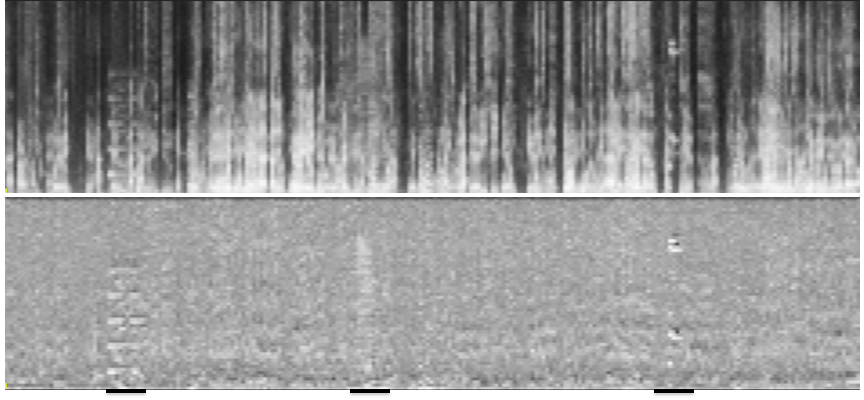
\includegraphics[width=0.95\linewidth]{figs/spectrogram-salience.png}
  \caption{Top: A normal spectrogram; Bottom: A salience-maximised spectrogram with target events marked using black
    underlines}
  \label{fig:timeliner}
\end{figure}

\section{Alternative audio visualisation}\label{sec:background-alternative}

One of the issues we identified with the above audio visualisations is that the user must interpret the data. Although
in many cases this can be learned, it requires cognitive load to process the images into the desired information. It
also means that novice users must be trained or gain sufficient experience to be able to reach satisfactory performance
levels.

Semantic audio is the extraction of meaning from audio. Example applications of semantic audio are speech-to-text or
music identification. This technology allows the computer to interpret the audio on the user's behalf in a way that is
helpful for their situation, however the success of this is dependent on the performance of the audio analysis
algorithm.

Semantic audio visualisation is a two-stage process where the audio is first analysed to extract the semantic data,
then the data is visualised. There are thousands of audio extraction and data visualisation techniques that could
be combined to create various audio visualisations. The interaction of these two parts, and the context of the
application, is important in the sucess of semantic audio visualisation. 

Below we consider semantic audio visualisation techniques that have attempted to aid navigation of audio content.

%\subsection{Segmentation}
%Music structure
%Speaker diarization

%\subsection{Transcription}
%Music transcription
%Speech to text

\subsection{Colour}\label{sec:background-colour}
A simple technique that can be used to visualise data is mapping numeric values to colour.  Previous work in the use of
colour for audio visualization can be categorised into two main approaches -- pseudocolour and false colour.

\paragraph{Pseudocolour}\label{sec:background-pseudocolour}
Pseudocolour is a method of mapping a scalar value to a colour gradient \citep{Moreland2009}.  A tangible example of
pseudocolour is thermal imaging cameras, where temperature is mapped to a colour gradient.  The gradient can be
composed of a two colours (e.g. from blue to red) or many colours (e.g. a rainbow).

Pseudocolour allows values to be mapped to colours that may be more perceptually relevant (e.g. green/red for
good/bad).  It also enables the full colour spectrum to be utilised, which can emphasize small variations between
values.  Non-linear gradients can be used to pick out particularly high or low values, and stepped gradients can be
used to separate values into categories.  However, as pseudocolour can only represent one dimension, it does not make
full use of the colour space.

Spectral waveform colouration has become an increasinly common feature in DJ software. It was first introduced with 
Serato Audio Research's `Scratch LIVE' program.
% TODO What year?
This feature allows DJs to use colour to distinguish between different drum noises, such as bass kicks, snares and
high-hats. Pseudocolour is used to enhanced the waveform, with spectral centroid used as the input audio feature.

The same technique has been applied to other applications, notably on the audio clip sharing website `Freesound' from
Universitat Pompeu Fabra's Music Technology Group\footnote{\url{http://blog.freesound.org/?p=10}, Bram de Jong, Music
  Technology Group, Universitat Pompeu Fabra, Barcelona}. In Freesound, coloured waveforms are used to help users
quickly find and compare sound effect and music clips on the website.

\paragraph{False colour}\label{sec:background-falsecolour}
False colour is where multiple values are mapped to the dimensions of a colour space. Commonly, three values are
mapped to the RGB (red, green, blue) colour space.  The advantage of this method is that it can make full use of the
available colours.  However, it can be challenging to select three values and map them to colour in a way that humans
can easily understand and interpret.

\citet{Tzanetakis2000} created a visualisation technique known as `Timbregrams' that aimed to ``use color perception
and the pattern recognition capabilities of the human visual system to depict timbral and temporal information''. Their
implementation mapped the first three principal components of a large feature vector to RGB colour space. The authors
claim that this approach matches sounds with similar `textures' to similar colours.
Although the authors didn't combine their algorithm with waveforms, this would be a simple step.

\citet{Rice2005} presented a similar idea to enhance waveforms with colour. The technique is not
explicitly defined, but it maps low/mid/high frequencies to blue/green/red. It was designed for identifying
timbrally distinct sounds and, with training, can be used to identify certain sound effects. Their system has since
been marketed and licensed as `Comparisonics' and has been integrated into commercial audio editing and DJ
software.

\begin{figure}[p]
\centering
\begin{subfigure}{\textwidth}
  \centering
  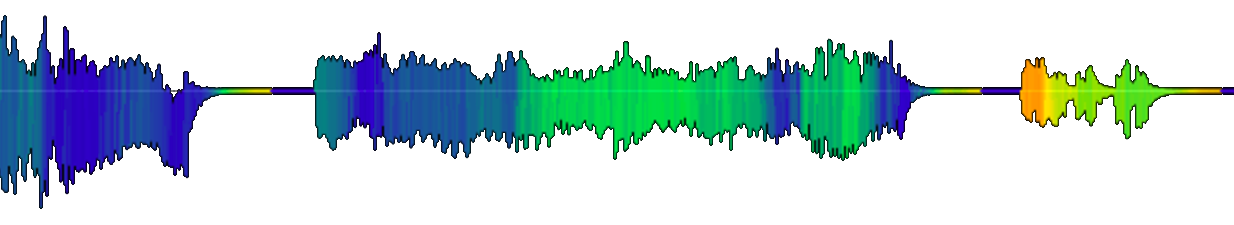
\includegraphics[width=\linewidth]{figs/freesound2.png}
  \caption{Freesound (\url{freesound.com})}
  \label{fig:freesound}
\end{subfigure}\\%
\begin{subfigure}{\textwidth}
  \centering
  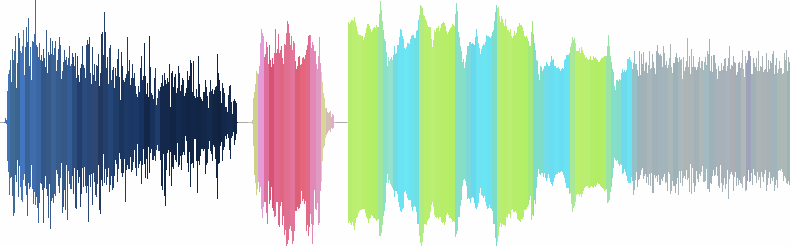
\includegraphics[width=\linewidth]{figs/rice.png}
  \caption{Comparisonics \citep{Rice2005}}
  \label{fig:rice}
\end{subfigure}
\caption{Examples of pseudocolour (\ref{fig:freesound}) and false colour
  (\ref{fig:rice}) applied to colourising an audio waveform}
\label{fig:colourvis}
\end{figure}

\citet{Mason2007} used false colour to assist radio listeners in navigating recently-broadcast material. They mapped
three empirically-chosen audio features to RGB colour space. The authors reported that the system was successful at
indicating the location of music within speech content, and highlighting low-bandwidth material such as phone calls.
The authors proposed that the system could be also be applied to other applications such as segmentation of radio
programmes for re-editing into podcasts.

%Similar work was conducted at the BBC in 2013 by trainee Andrew Bonney who,
%under the supervision of the author, looked into whether colour could represent
%the sound of different people's voices. The result used median-filtered MFCCs
%and gaussian mixture models, mapped to RGB colour space.
%Figure~\ref{fig:bonney} shows an example of a recording with three speakers
%(red/orange, blue and light/dark green).

%\begin{figure}[ht]
  %\centering
  %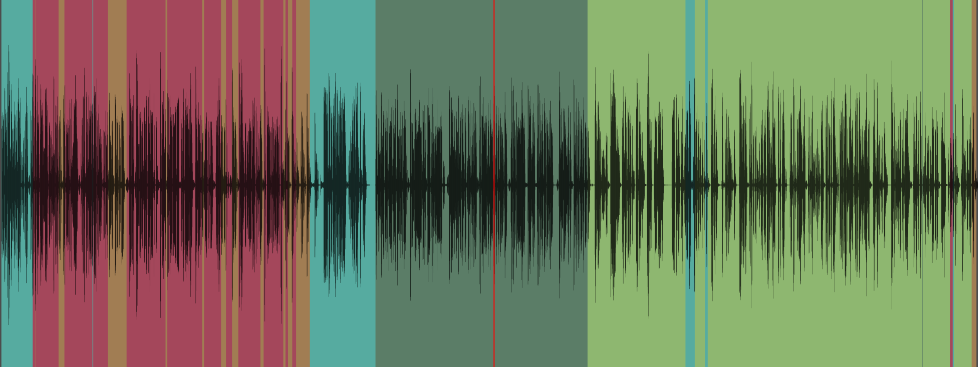
\includegraphics[width=0.95\linewidth]{figs/bonney.png}
  %\caption{Speaker diarizartion through colour based on filtered MFCCs}
  %\label{fig:bonney}
%\end{figure}

False colour has also been used for navigating and summarizing extremely long recordings. \citet{Towsey2014} mapped
three spectral features to RGB colour for visualizing almost a year of environmental recording.
Figure~\ref{fig:towsey} shows the recordings from March until October, with each line representing one day.  The
visualization reveals the change in time of the dawn and evening choruses throughout the year, amongst other things.

\begin{figure}[p]
  \centering
  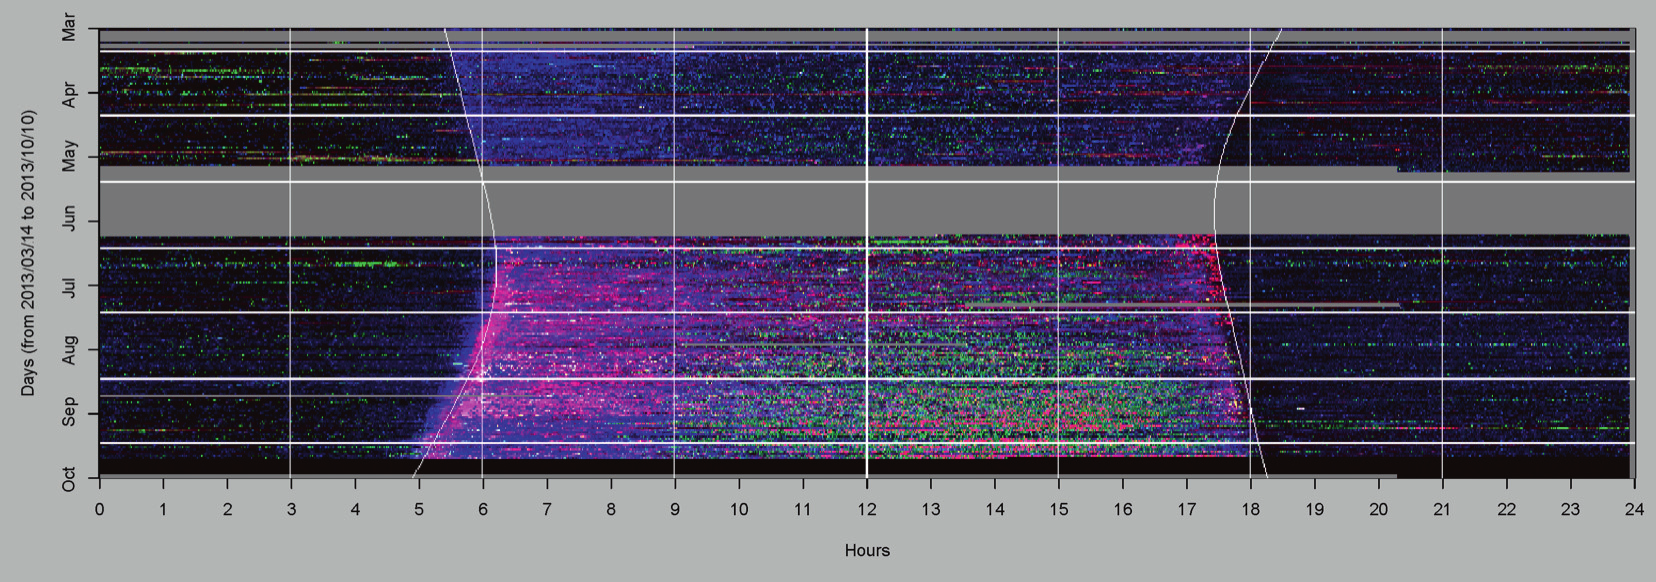
\includegraphics[width=0.95\linewidth]{figs/towsey.png}
  \caption{False colour visualization of environmental recordings, with each line representing one day. Missing data is
    shown in grey.
    \citep{Towsey2014}}
  \label{fig:towsey}
\end{figure}

\subsection{Segmentation}

Speech/music discrimination \citep{Wieser2014}

\subsection{Summarization}

Extracting keyphrases \citep{Inkpen2004}
TreeMaps \citep{Abdulhamid2013a}
World service archive \citep{Raimond2014}

\subsection{Transcripts}

LIDS transcript editor \citep{Apperley2002}

Editor for existing script \citep{Shin2016}


\section{Auditory and haptic interfaces}\label{sec:background-auditory}

SpeechSkimmer \citep{Arons1997}

Dichromatic listening \citep{Ranjan2006}

Haptics
\citep{Metatla2016}

%======================================================================================================================

%Academic research into audio analysis and audio interfaces tends to concentrate
%on fully automated systems \citep{AngueraMiro2012}, navigation of large audio
%collections \citep{FontCorbera2010} or navigation interfaces based on skimming
%\citep{Arons1997} and scrolling \citep{Lee2007}. Although there are examples of
%audio visualization from the world of academia, it is much more popular in the
%context of art \citep{Armitage2012}, with excellent examples such as Quayola's
%Form--Sound--Abstraction\footnote{\url{http://www.quayola.com/work/form-sound-abstraction/}}
%work.

%This section looks at three areas of literature from which the project will
%draw upon -- extraction of meaningful audio properties, mapping these to a
%visual representation, and the perceptual links between audition and vision.

%\section{Feature extraction}\label{sec:litreviewfeats}
%This section looks at audio features that could be used as part of an audio
%visualization system. Firstly, two use cases that were previously identified as
%being a common component of radio production are explored, before considering
%methods of generating features for any use case.

%\subsection{Speech/music discrimination}
%Speech/music discrimination (SMD) is the process of segmenting audio content
%into parts labelled by the categories speech and music. In general, SMD
%classifiers use a collection of different features. This section lists the ones
%that are used frequently or have recently been found to perform well.

%\paragraph{RMS energy}
%The root mean squared energy can be used also exclusively as an effective SMD
%classifier, as demonstrated in \citep{Ericsson2009} and \citep{Panagiotakis2005}.
%Commonly used statistics of RMS include low energy ratio
%\citep{Liang2005,Ericsson2009,Saunders1996,Scheirer1997} and variance
%\citep{Ericsson2009} (including normalised variance \citep{Panagiotakis2005} and
%delta variance \citep{Carey1999}).

%Low energy ratio (also known as `silent interval frequency' and `energy contour
%dip') is a measure of the number of RMS energy frames that fall below a
%threshold. It exploits the fact that speech has freqent silent gaps between
%words, wheras music does not. The threshold can be set as a fixed value
%\citep{Liang2005}, a function of a moving average \citep{Ericsson2009} or moving
%peak value \citep{Saunders1996}.

%Kacprzak and Zi\'{o}\l{}ko recently proposed a modified version of low energy
%ratio called `minimum energy density' \citep{Kacprzak2013}. It is calculated by
%normalizing over a $\sim$15 second window and finding the minimum of the
%normalization function over a $\sim$1--3 second window. It has similar
%performance to low energy ratio with a moving average threshold, but has fewer
%parameters to set.

%\paragraph{Zero-crossing rate} is the rate at which a signal crosses the time
%axis, which is an easy-to-calculate measure for the spectral energy
%distribution. Early work in SMD \citep{Saunders1996} identified that ``speech
%signals produce a marked rise in the ZCR during periods of fricativity occuring
%at the beginning and end of words'', wheras music does not. This causes a
%bimodality which skews the ZCR distribition, which can be measured using the
%third standardized moment (skewness). The variance of ZCR has also been found
%to perform well for SMD \citep{Scheirer1997}.

%ZCR also played a significant role in two steps of a five-step classifer
%\citep{Panagiotakis2005}. During silent intervals the number of zero crossings
%is null, so this was used to detect gaps between speech. The authors also noted
%that ``RMS and ZCR are somewhat correlated for speech signals, while
%essentially independent for music'', and so the product of RMS and ZCR was used
%for the second classifier.

%A review \citep{Carey1999} of features for SMD found ZCR to perform least well,
%but did not consider the skewness, variance, or probability of null
%zero-crossings.

%\paragraph{MFCC}
%Mel-frequency cepstral coefficients have long been the workhorse of audio
%analysis, and they have been successfully used in SMD applications
%\citep{Carey1999,Liang2005,Pikrakis2008,Pikrakis2006a,Sell2014,Wieser2014}.
%Notably, their use has only been successful when used in combination with
%strong machine learning systems, indicating that the relationship of MFCCs to
%SMD labels is complex and non-linear. This would make it difficult to map to a
%visual representation.

%\paragraph{Chroma}
%Use of chroma features work on the principle that the spectra of music is
%aligned to the chromatic scale. Pikrakis et. al.
%\citep{Pikrakis2006,Pikrakis2008} have successfully used `chromatic entropy' for
%SMD applications. It takes sub-bands from a mel-scaled spectrum, aligned to the
%chromatic scale, and calculates the entropy of the normalised spectral energy.

%More recently, Sell \citep{Sell2014} has proposed two new chroma features, which
%try to account for the fact that the chromagram varies greatly between
%different pieces of music. Music tends to form strong, separated peaks on the
%chromagram wheras speech has smoother mounds of energy. The new features
%attempt to measure the peakiness of the chromagram. `Chromatic diff' subtracts
%a shifted chroma vector from the original chroma vector and sums the energy. 
%`Chroma high freq' performs an FFT on the chromagram and sums the high
%frequency energy.

%\paragraph{Continuous frequency activation}
%Most of the above SMD features work well for segmenting speech-only/music-only
%content. However, many fall down at detecting background music in speech.
%Seyerlehner developed the continuous frequency activation (CFA) feature
%\citep{Seyerlehner2007}, which works on the basis that music content has stable
%harmonics, seen as horizontal lines on a spectrogram.

%A moving average is subtracted from the FFT before it is binarized using a low
%threshold value. For each bin, the proportion of active frames in an analysis
%window is counted. The result is analysed with a peak picking algorithm and the
%sum of the five largest peaks are used as the CFA. The result is a single
%numeric value which quantifies the presence of steady frequency components.

%In the original CFA paper, the feature was used to find music in television
%content, but recently it has also been successfully applied to segmentaton of
%radio recordings \citep{Wieser2014}.

%\subsection{Speaker diarization}
%Speaker diarization is the process of segmenting a speech recording by where
%different people are talking. Review papers from 2006 \citep{Tranter2006} and
%2012 \citep{AngueraMiro2012} show that the vast majority of systems are based on
%clustering of MFCC or PLP features, which are low-dimensional representations
%of speech. Rather than developing new features, the research is primarily
%focussed on improvement of the clustering algorithms and pre-processing stages
%such as Wiener filtering, speech activity detection and beamforming.

%MFCC and PLP features are extremely effective when used in machine-based
%classification systems, but from a human perception angle, the features do not
%correlate well to what is heard.  Other features developed for automatic speech
%recognition may also be useful in a speaker diarization system. For example,
%spectral entropy \citep{Misra2004} is a measure of the peakiness of the spectrum
%and is an effective feature in distinguishing between voiced and unvoiced
%speech.

%Friendland et. al. \citep{Friedland2009} proposed enhancing the standard MFCC
%features with a set of long-term features representing prosody (the rhythm and
%intonation of speech). 52 candidate features were ranked using feature
%selection, which showed that ``the median and mean fundamental frequency are
%the best features, following by high formants (F4, F5)''. Inclusion of the
%top ten prosodic features improved the speaker diarization system by 24\%.

%\subsection{Feature generation}\label{sec:litreviewgeneration}
%Traditionally, audio features were developed by hand for specific tasks. This
%was usually done by attempting to write an algorithm that calculated the
%properties of the sound that humans used to distinuish the categories in
%question. More recently, fuelled by an ever-increasing availability of
%computing power, research has had a much greater focus on automating
%this process.

%\paragraph{Feature selection/extraction}
%Feature selection and extraction are methods of reducing the dimensionality of
%a feature vector, either by choosing a combination of vector components that
%best describe the content (selection), or by translating the feature vector to
%a smaller vector while retaining as much information as possible (extraction).

%This process can be unsupervised where only the feature data is known (such as
%with principal component analysis), or supervised where the feature data has
%corresponding labels (such as with linear discriminant analysis).

%Canonical correaltion analysis (CCA) has been used to reduce the dimensions of
%features for speaker diarization \citep{Chaudhuri2009} and phonetic labelling
%\citep{Arora2014}, amongst other things. It is able to efficiently map features
%to a subspace and can be used with the kernel trick (known as KCCA) to support
%non-linear mappings. In the case of speaker clustering, ``CCA-based algorithms
%consistently provide better performance than standard PCA-based clustering
%methods'' \citep{Chaudhuri2009}.

%\paragraph{Feature learning}
%The above methods of reducing dimensionality are based on a relatively short
%information-rich feature vector that it suitable for the target application.
%More recent research on feature development is focussed on automated learning
%of features using large labelled datasets.

%Deep learning is an increasingly popular method of learning features based on
%neural networks with large numbers (tens or hundreds) of hidden units. This
%line of research has been enabled by the increasing availability of large
%amount of processing power. When done properly, deep learning can produce the
%state-of-the-art in audio features, outperforming even the best hand-crafted
%features \citep{Hamel2010,Sigtia2014}.

%Such an approach requires a high-quality and very large labelled dataset, on
%which the success of the process depends. The nature of neural networks means
%that it is very difficult to interpret what the resulting features represent
%which isn't an issue when used as the input to a machine learning system, but
%would make it very difficult to map to a visualization. The objective of the
%deep learning process is to minimise a cost function rather than to maximise
%the link to human perception.


\chapter{Navigation of audio waveforms}\label{sec:study}
Conducting experiments online brings a range of benefits as they can be run in
parallel, taken at any time at any place, and are easily shared. Recent
advances in web technology standards (notably
HTML5\footnote{\url{http://www.w3.org/TR/html5/}}) mean that it is now
possible to implement advanced audio interfaces on a wide range of browsers,
making large scale evaluation achievable.

\section{Goals}
The primary objective of this initial experiment was to verify that conducting
a task-based evaluation of an audio interface online is viable and produces
significant results. It was designed to have a narrow scope and low requirement
for participants so that any problems could be identified without having to
involve large amounts of people.

The context of the experiment was to evaluate the performance of the most
common method of visualising audio -- the waveform -- and investigate whether
there is potential to improve upon it.

\section{Experimental design}
In order to attract a sufficient number of participants while collecting enough
data, the experiment was designed so it could be completed in 10--15 mins.

\subsection{Task}\label{sec:studytask}
The experiment was designed to simulate a typical task encountered by radio
producers. Creation of podcasts is a common but often tedious exercise for
producers which primarily involves finding each piece of music played in a
programme and editing them down to 30 seconds in length. This is in order to
comply with rights agreements for downloadable content.

Although it is possible for experienced producers to distinguish between music
and speech using a waveform, this representation doesn't scale very well so it
becomes very difficult when the display is zoomed-out. As such, finding music
at the programme level can be challenging.

The task for the experiment was to find and select the piece of music content
in a recording of a radio programme.

\subsection{Conditions}
Three different methods were used to visualize the audio: a normal waveform, a
task-enhanced waveform and a blank display (no waveform). The blank
visualization acts as a baseline where participants are operating `blind' with
no visual assistance. The enhanced waveform (see
Section~\ref{sec:studywaveform}) represents a nominal improvement using a
simple algorithm designed for the task.

The expected result is that having a waveform is better than having nothing,
and that an enhanced waveform performs better than a normal waveform.

\subsection{Test data}
The radio programme recordings were selected to represent the wide variety of
programme and music genres broadcast on the radio, as well as covering both
male and female speakers and a range of different radio stations.

The audio content was sourced from internal BBC recordings of transmission
(ROT) and were edited to be approximately five mins in length, and to have only
one section that could be categorised as music.

The programmes are described in Table~\ref{tab:clips}.

\begin{table}[htbp]
  \begin{center}
    \begin{tabular}{|r|l|l|l|l|l|}
      \hline
      \multicolumn{1}{|l|}{\textbf{Clip}} & \textbf{Network} & \textbf{Title} &
      \textbf{Voices} & \textbf{Prog genre} & \textbf{Music genre} \\ \hline
      Train & Radio 4 & Desert Island Discs & Female & Interview & Ambient \\ \hline
      1 & 1 Xtra & Sian Anderson & Male, Female & Breakfast & Dance \\ \hline
      2 & 6 Music & Lauren Laverne & Female & Single & Indie \\ \hline
      3 & Radio 2 & Ken Bruce & Male & Phone quiz & Lounge \\ \hline
      4 & Radio 3 & Breakfast show & Male & Single & Classical \\ \hline
      5 & 5 Live & Sports report & Male & Sports & Band \\ \hline
      6 & Radio 1 & Zane Lowe & Male & Interview & Rap \\ \hline
      7 & Radio 2 & Jo Whiley & Male, Female & Review & Pop \\ \hline
      8 & Radio 4 & Afternoon drama & Male, Female & Drama & Classical \\ \hline
      9 & Radio 4 & Front Row & Male & Interview & Alternative \\ \hline
    \end{tabular}
  \end{center}
  \caption{Descriptions of the radio programmes used for the evaluation}
  \label{tab:clips}
\end{table}

\subsection{Measures}\label{sec:measures}
\paragraph{Demographics}
Participants were asked about their gender, age and a number of question which
attempted to gauge their level of experience. The questions and options are
listed below:

{\singlespacing
\begin{itemize}
  \item Do you understand what an audio waveform is? [Yes/No]
  \item Have you previously used any consumer audio editing software? (e.g.
    Audacity, GarageBand) [Yes/No]
  \item Have you previously used any professional audio editing software? (e.g.
    ProTools, Logic, Cubase/Nuendo, SADiE, Startrack) [Yes/No]
  \item How many years (if any) have you worked with audio in a professional
    capacity? [\textit{number}]
\end{itemize}
}

\paragraph{Performance metrics}
The interface was configured to log every action the user made. This was done
by recording time-stamps, so that not only can the number of actions be counted,
but the timing and frequency of the actions can also be measured.

The actions that were recorded are listed below:

{\singlespacing
\begin{itemize}
  \item Seek (top display)
  \item Seek (bottom display)
  \item Play/pause
  \item Select (using button)
  \item Select (using slider)
  \item Zoom in
  \item Zoom out
  \item Task completion
\end{itemize}
}

\paragraph{Task load}
After completing the tasks for a given condition, participants were asked to
rate the tasks using the NASA Task Load Index (NASA-TLX) \cite{Hart1988}
metrics on a scale of $-10$ to $+10$. These are listed below:

{\singlespacing
\begin{itemize}
  \item Mental Demand -- How mentally demanding was the task? [very low/very
    high]
  \item Physical Demand -- How physically demanding was the task? [very
    low/very high]
  \item Temporal Demand -- How hurried or rushed was the pace of the task?
    [very low/very high]
  \item Performance -- How successful were you in accomplishing what you were
    asked to do? [perfect/failure]
  \item Effort -- How hard did you have to work to accomplish your level of
    performance? [very low/very high]
  \item Frustration -- How insecure, discouraged, irritated, stressed, and
    annoyed were you? [very low/very high]
\end{itemize}
}

\paragraph{Comparison}
At the end of the experiment, participants were asked to compare the conditions
directly by selecting which they thought were the easiest and most frustrating.
A thumbnail image representing each visualisation was shown to remind the
participants of how they looked.

\paragraph{Other}
In addition to the above measures, the browser and operating system each
participant used was recorded, as was the date and time at which they
submitted each data point.

\subsection{Sequence}\label{sec:studysequence}
In order to make it possible for the experiment to completed in 10-15 mins, a
sequence of nine tasks was used. The conditions were grouped rather than mixed
(e.g. AAABBBCCC instead of ACACBABCB) in order to avoid confusion when
switching between them. The TLX questions were presented after each group of
conditions (i.e. AAATBBBTCCCT) and the comparison questions were presented at
the end.

Each audio clip can only be used once per participant, otherwise they would be
able to remember where the music was. An efficient way of presenting each clip
once is to use a Latin square. A Latin square is an $n \times n$ array with $n$
different symbols, with each symbol occurring exactly once in each row and
exactly once in each column. A Williams design Latin square \cite{Williams1949}
is one which is balanced for first order carryover effects.  When $n$ is odd,
to maintain balance two Latin squares must be used, producing a $2n \times n$
array.

For the sequence of 9 audio clips, an $18\times9$ Williams design Latin square
was used (see Table~\ref{tab:clipseq}), which was generated using the
\texttt{crossdes}
package\footnote{\url{http://cran.r-project.org/web/packages/crossdes/index.html}}
in R. The visualisation sequence was generated by modifying this design. First,
the middle three columns\footnote{It was determined empirically that the
  middle 3 columns were the optimum selection when used as described} were
extracted, and the values $4-6$ and $7-9$ were mapped to $1-3$. The resulting
$18\times3$ matrix was then expanded horizontally to produce a $18\times9$
matrix (see Table~\ref{tab:visseq}). When the two sequences are combined, the
result is balanced and has minimal carryover effects.

\begin{table}
  \parbox{.45\linewidth}{
    \centering
    \begin{tabular}{rrrrrrrrr}

      1 & 2 & 9 & 3 & 8 & 4 & 7 & 5 & 6 \\ 
      2 & 3 & 1 & 4 & 9 & 5 & 8 & 6 & 7 \\ 
      3 & 4 & 2 & 5 & 1 & 6 & 9 & 7 & 8 \\ 
      4 & 5 & 3 & 6 & 2 & 7 & 1 & 8 & 9 \\ 
      5 & 6 & 4 & 7 & 3 & 8 & 2 & 9 & 1 \\ 
      6 & 7 & 5 & 8 & 4 & 9 & 3 & 1 & 2 \\ 
      7 & 8 & 6 & 9 & 5 & 1 & 4 & 2 & 3 \\ 
      8 & 9 & 7 & 1 & 6 & 2 & 5 & 3 & 4 \\ 
      9 & 1 & 8 & 2 & 7 & 3 & 6 & 4 & 5 \\ 
      6 & 5 & 7 & 4 & 8 & 3 & 9 & 2 & 1 \\ 
      7 & 6 & 8 & 5 & 9 & 4 & 1 & 3 & 2 \\ 
      8 & 7 & 9 & 6 & 1 & 5 & 2 & 4 & 3 \\ 
      9 & 8 & 1 & 7 & 2 & 6 & 3 & 5 & 4 \\ 
      1 & 9 & 2 & 8 & 3 & 7 & 4 & 6 & 5 \\ 
      2 & 1 & 3 & 9 & 4 & 8 & 5 & 7 & 6 \\ 
      3 & 2 & 4 & 1 & 5 & 9 & 6 & 8 & 7 \\ 
      4 & 3 & 5 & 2 & 6 & 1 & 7 & 9 & 8 \\ 
      5 & 4 & 6 & 3 & 7 & 2 & 8 & 1 & 9 \\ 
    \end{tabular}
    \caption{Audio clip sequence -- each row is a test sequence}
    \label{tab:clipseq}
  }
  \hfill
  \parbox{.45\linewidth}{
    \centering
    \begin{tabular}{rrrrrrrrr}

      3 & 3 & 3 & 2 & 2 & 2 & 1 & 1 & 1 \\ 
      1 & 1 & 1 & 3 & 3 & 3 & 2 & 2 & 2 \\ 
      2 & 2 & 2 & 1 & 1 & 1 & 3 & 3 & 3 \\ 
      3 & 3 & 3 & 2 & 2 & 2 & 1 & 1 & 1 \\ 
      1 & 1 & 1 & 3 & 3 & 3 & 2 & 2 & 2 \\ 
      2 & 2 & 2 & 1 & 1 & 1 & 3 & 3 & 3 \\ 
      3 & 3 & 3 & 2 & 2 & 2 & 1 & 1 & 1 \\ 
      1 & 1 & 1 & 3 & 3 & 3 & 2 & 2 & 2 \\ 
      2 & 2 & 2 & 1 & 1 & 1 & 3 & 3 & 3 \\ 
      1 & 1 & 1 & 2 & 2 & 2 & 3 & 3 & 3 \\ 
      2 & 2 & 2 & 3 & 3 & 3 & 1 & 1 & 1 \\ 
      3 & 3 & 3 & 1 & 1 & 1 & 2 & 2 & 2 \\ 
      1 & 1 & 1 & 2 & 2 & 2 & 3 & 3 & 3 \\ 
      2 & 2 & 2 & 3 & 3 & 3 & 1 & 1 & 1 \\ 
      3 & 3 & 3 & 1 & 1 & 1 & 2 & 2 & 2 \\ 
      1 & 1 & 1 & 2 & 2 & 2 & 3 & 3 & 3 \\ 
      2 & 2 & 2 & 3 & 3 & 3 & 1 & 1 & 1 \\ 
      3 & 3 & 3 & 1 & 1 & 1 & 2 & 2 & 2 \\ 
    \end{tabular}
    \caption{Visualization sequence -- each row is a test sequence}
    \label{tab:visseq}
  }
\end{table}

\section{Method}

\section{Interface design}
An online audio interface and evaluation system was developed, which is
described in detail in Section \ref{sec:iface}. It displays two audio
visualisations -- one shows the full recording, and the other shows a zoomed-in
view. Basic functionality was implemented, including seek, zoom, play/pause and
selection.

\subsection{Enhanced waveform}\label{sec:studywaveform}
The enhanced waveform was created by modifying the colour of a standard
waveform, based on a very simple speech/music discrimination (SMD) feature.

As shown in Section~\ref{sec:litreview}, low energy ratio is a popular, simple
and effective scalar metric for speech/music discrimination. It works on the
principle that speech has intermittent silences (between words) whereas music
does not. It was calculated by extracting the RMS energy (20ms frames, no
overlap) and counting the proportion of frames which fall below a threshold.
In the case of this experiment, the threshold was configured as the third
percentile of RMS energy in a one second sliding window. These parameters were
set empirically by testing them against radio programme recordings.

The low energy ratio was mapped to a colour gradient which was blue for low
values (representing speech) and to pink for high values (representing music).
The shade of blue was chosen to match that used in StarTrack and the pink is
it's inverse colour.

\subsection{Promotion}\label{sec:promo}
The experiment was promoted using two email lists which covered all staff in
BBC Research and Development (approx. 150 people) and all residents in the
Electronics and Computer Science department at Queen Mary University of London
(approx. 300 people). Although there are a large number of audio specialists
working in both groups, the recipients are mostly non-experts.

\subsection{Ethics}
Ethics approval for the experiment was gained from the QMUL Research Ethics
Committee and is logged under the reference \texttt{QMREC1348d}. Due to the
low-risk nature of the study, this was done through expedited review. The
consent form presented to participants in the study is reprinted in
Appendix~\ref{app:consent}.

\section{Results}
63 responses were completed in the three weeks the experiment ran. Emails
linking to the experiment were sent to roughly 450 people, which gives a
conversion rate of 14\%. This is much higher than was expected.  Informal
feedback suggested that many people enjoyed participating due to the listening
and task-based nature of the experiment. 

\subsection{Validation}
In order to ensure that participants were following the instructions correctly,
they were filtered using an acceptance criteria (see Figure~\ref{eq:accept}).
It stipulates that any participant who submits a response with an absolute
error of more than 5 seconds is rejected.

\begin{figure}[ht]
  \begin{center}
    $ |t_{in}-t_{inREF}| + |t_{out}-t_{outREF}| \leq 5 $
  \end{center}
  \caption{Acceptance criteria, where $t_{in}$ and $t_{out}$ are the in and out
    points of each selection, and $t_{inREF}$ and $t_{outREF}$ are the ground
    truth in and out points}
  \label{eq:accept}
\end{figure}

Of the 63 experiments completed, only 41 passed the above criteria meaning that
35\% of participants were rejected. Figure~\ref{fig:rejectdaw} shows that none
of the rejected participants had experience of using a professional audio
editor, suggesting that the mistakes may have been made due to inexperience
with audio interfaces.

\begin{figure}[ht]
  \centering
  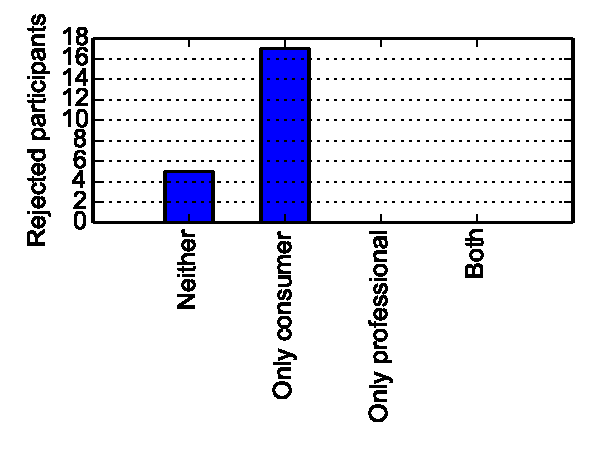
\includegraphics[width=0.5\textwidth]{figs/reject-daw.pdf}
  \caption{Response of rejected participants when asked whether they had
    previously used consumer/professional audio editing software}
  \label{fig:rejectdaw}
\end{figure}

Figure~\ref{fig:rejectvis} plots the number of incorrect responses received for
each visualisation, which shows that no particular visualisation is responsible
for the mistakes. However, Figure~\ref{fig:rejectclip} shows that there is
variation in the mistakes made for each clip, particularly clips 4 and 5. An
analysis of the incorrect in and out points for these clips found that
the mistakes were varied and don't suggest a systematic problem. 

\begin{figure}[ht]
\centering
\begin{subfigure}{.5\textwidth}
  \centering
  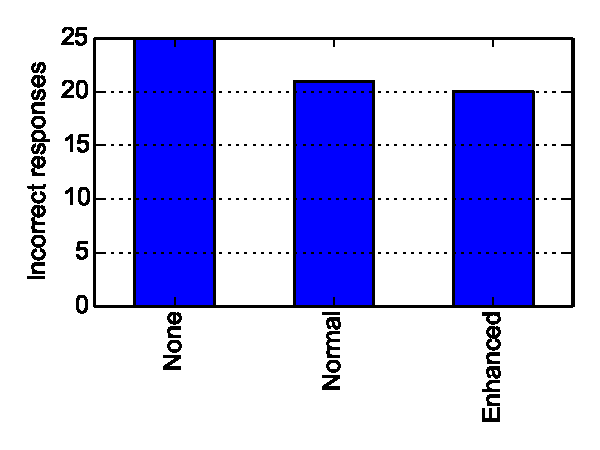
\includegraphics[width=\linewidth]{figs/rejects-vis.pdf}
  \caption{By visualisation}
  \label{fig:rejectvis}
\end{subfigure}%
\begin{subfigure}{.5\textwidth}
  \centering
  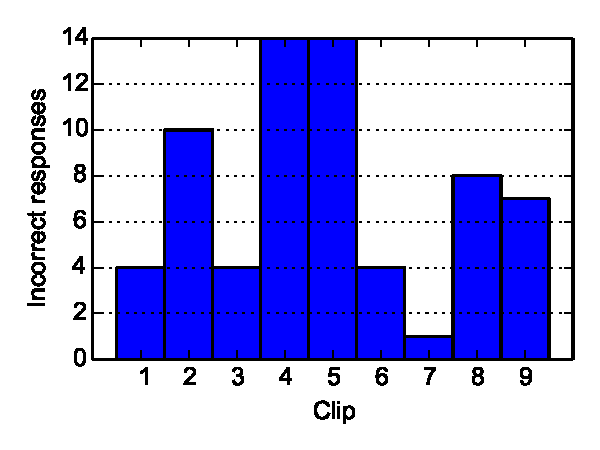
\includegraphics[width=\linewidth]{figs/rejects-clip.pdf}
  \caption{By clip}
  \label{fig:rejectclip}
\end{subfigure}
\caption{Analysis of incorrect responses}
\label{fig:rejects}
\end{figure}

\subsection{Demographics}
The demographic of the participants showed a heavy bias (80\%) of male
participants, and a larger proportion in the 26-45 age range (see
Figure~\ref{fig:age}). This reflects the population to which the experiment was
promoted (see Section~\ref{sec:promo}) and is not expected to skew the results.

\begin{figure}[ht]
  \centering
  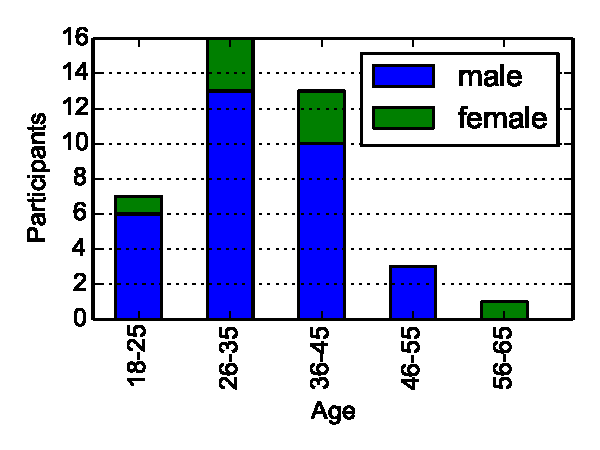
\includegraphics[width=0.5\textwidth]{figs/age.pdf}
  \caption{Age and gender of participants. Male/female ratio was 32/8
    (80\%/20\%). One participant declined to respond to the question.}
  \label{fig:age}
\end{figure}

Most participants had previous experience of using both consumer and
professional audio editing software (see Figure~\ref{fig:experiencedaw}), with
29\% of participants only having experience of consumer software or no
experience at all.

When asked about years of professional audio experience, 39\% of participants
reported having no experience, with the remainder being spread out up to a
maximum of 25 years (see Figure~\ref{fig:experienceyears}). Interestingly, the
answer people gave peaks at the 5 and 10--year marks, where people may have
given a rounded number rather than an accurate figure.

\begin{figure}[ht]
\centering
\begin{subfigure}{.5\textwidth}
  \centering
  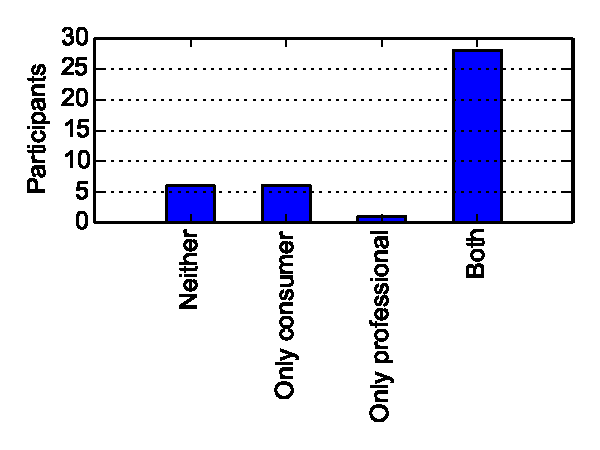
\includegraphics[width=\textwidth]{figs/daw.pdf}
  \caption{Previous use of audio editing software}
  \label{fig:experiencedaw}
\end{subfigure}%
\begin{subfigure}{.5\textwidth}
  \centering
  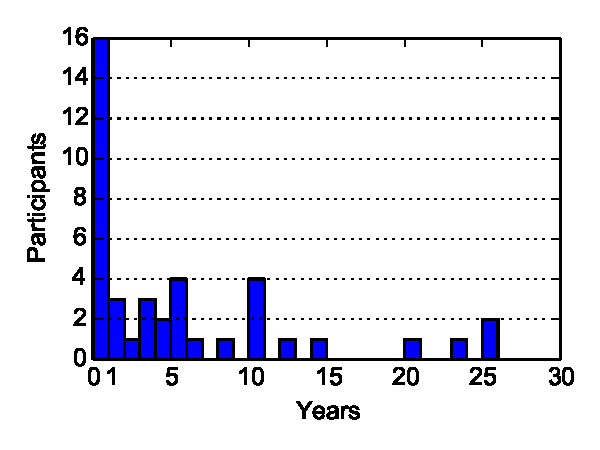
\includegraphics[width=\linewidth]{figs/experience.pdf}
  \caption{Years of professional audio experience}
  \label{fig:experienceyears}
\end{subfigure}
\caption{Response of participants to questions about experience}
\label{fig:experience}
\end{figure}

\subsection{Analysis methods}
This section describes the various tools that were used to analyse the data
collected using the experiment, find differences between conditions and
determine whether they are of significance.

\paragraph{Box plot}
A box plot \cite{McGill1978} is a technique used to graph distributions by 
their quartile values (i.e. 25th, 50th and 75th percentiles). An example can be
seen in Figure~\ref{fig:seekbox}. The box extends from the first to the third
quartile, with the second quartile (median) marked as a line through the box.
Lines are drawn from the box to the minimum and maximum, known as `whiskers',
however data determined to be outliers are marked separately as crosses.
The 95\% confidence interval of the median is marked as a notch in the box.

\paragraph{ANOVA}
Analysis of variance is a method of testing whether the mean values of several
groups are equal or not. It assumes that the observations are independent, that
the data have a normal distribution, and that the variance within the groups
are similar. One-way ANOVA tests for a null hypothesis that the means values of
the factors are the same.

\paragraph{Tukey's test}
If the null hypothesis is rejected using ANOVA, we know that there is a
difference between the factors, but we don't know which ones. Tukey's test is a
post-hoc analysis for discovering the difference between individual factors.
It assumes that the observations are independent and that the variance within
the groups are similar.

When Tukey's test is graphed, the mean values are represented by a dot with a
line either side showing the confidence interval. Confidence intervals which
don't overlap can be said to be significantly different.

\paragraph{Standardisation}
Some observations can be biased through participant behaviour. For example,
person A navigates audio recordings by quickly clicking along the timeline
while person B navigates with only a few considered clicks. To block this
factor, the responses of each participant can be standardised so that they have
a mean value of 0 and a standard deviation of 1. This allows the difference
between different participants responses to be measured fairly.

Standardisation maps observations to the `\textbf{standard score}'. This is a
dimensionless unit which represents the number of standard deviations an
observation is above the mean.

\subsection{Performance metrics}\label{sec:studymetrics}
An analysis was carried out on the performance metrics that were measured while
participants used the interface (see Section~\ref{sec:measures}).

\paragraph{Seek action}
The number of seek actions made was standardised for each participant. This was
done to reduce variation due to different search styles (i.e. frequent aimless
seeking along the timeline vs. infrequent purposeful seeking)

ANOVA found there to be a difference between the visualizations for $p < 0.01$
and Tukey's HSD test (see Figure~\ref{fig:seektukey}) showed that the number of
seek actions are different for each visualization in favour of the enhanced
version, again for $p < 0.01$. Even without standardisation, the same result
holds for $p < 0.05$.

\begin{figure}[ht]
\centering
\begin{subfigure}{.5\textwidth}
  \centering
  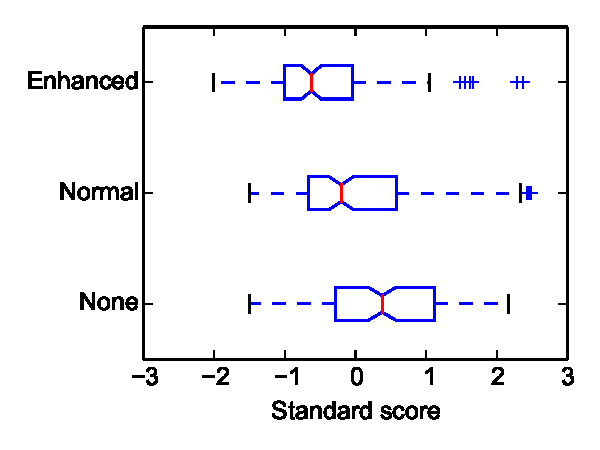
\includegraphics[width=\textwidth]{figs/seek-std.pdf}
  \caption{Box plot}
  \label{fig:seekbox}
\end{subfigure}%
\begin{subfigure}{.5\textwidth}
  \centering
  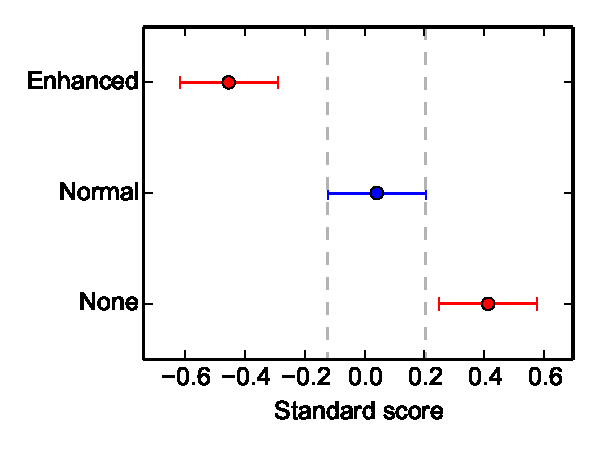
\includegraphics[width=\linewidth]{figs/seek-std-tukey99.pdf}
  \caption{Tukey's test (99\% confidence interval)}
  \label{fig:seektukey}
\end{subfigure}
\caption{Number of seek actions, standardised per participant}
\label{fig:seek}
\end{figure}

\paragraph{Selection time}
The time taken to make a selection was calculated as the difference between the
time the play button was first pressed and the time the final selection was
made. This reduces variation due to participants not starting the task
immediately and participants who made a selection, then checked the rest of the
recording for other pieces of music. The mean and standard deviation of the
selection time was standardised for each participant to reduce the effect of
people's natural pace.

\begin{figure}[ht]
\centering
\begin{subfigure}{.5\textwidth}
  \centering
  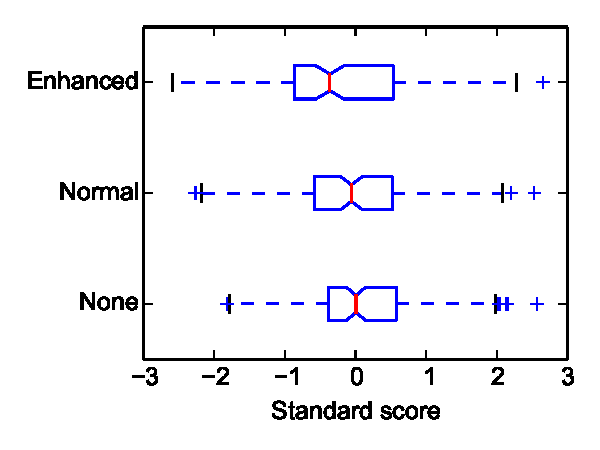
\includegraphics[width=\textwidth]{figs/playstart-to-selectend-std.pdf}
  \caption{Box plot}
  \label{fig:selecttimebox}
\end{subfigure}%
\begin{subfigure}{.5\textwidth}
  \centering
  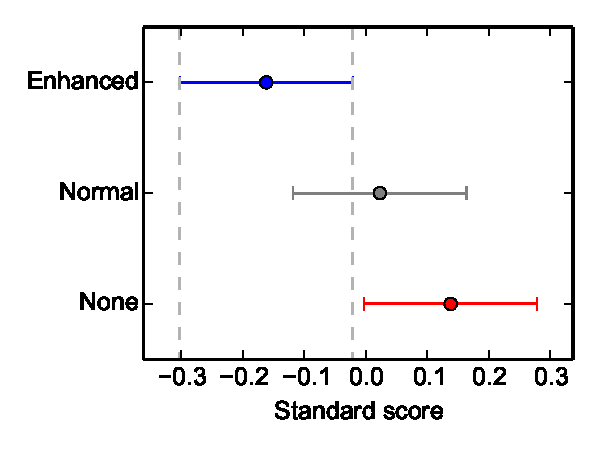
\includegraphics[width=\linewidth]{figs/playstart-to-selectend-std-tukey95.pdf}
  \caption{Tukey's test (95\% confidence interval)}
  \label{fig:selecttimetukey}
\end{subfigure}
\caption{Selection time (time between start of playback and final selection),
    standardised per participant}
\label{fig:selecttime}
\end{figure}

ANOVA showed that there was a significant difference between visualizations for
$p < 0.05$. Tukey's test (see Figure~\ref{fig:selecttimetukey}) found that
there was a difference between no visualization and the enhanced version, but
not between either of them and the normal waveform.

\paragraph{Error}
The absolute error of the selections made by each participant were calculated
for the inpoint, outpoint and sum of both. ANOVA found there to be no
difference between the visualisations for the inpoint or the sum, but found a
significant difference ($p < 0.05$) for the outpoint.  Tukey's test (see
Figure~\ref{fig:outpointerrtukey}) found that the absolute error of the
outpoint for the enhanced visualization was significantly lower than the other
two visualizations, but that the other two were no different.

This is an unexpected result which is difficult to explain, as the inpoint and
sum errors were not even close to rejecting the null hypothesis ($p > 0.3$).
Although the result is significant, the improvement in accuracy is only about
150ms which is small in the context of 5-minute recordings.

\begin{figure}[ht]
\centering
\begin{subfigure}{.5\textwidth}
  \centering
  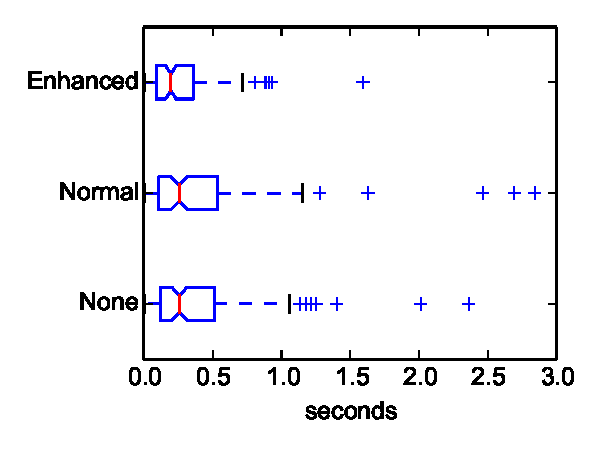
\includegraphics[width=\textwidth]{figs/outpoint-abserr.pdf}
  \caption{Box plot}
  \label{fig:outpointerrbox}
\end{subfigure}%
\begin{subfigure}{.5\textwidth}
  \centering
  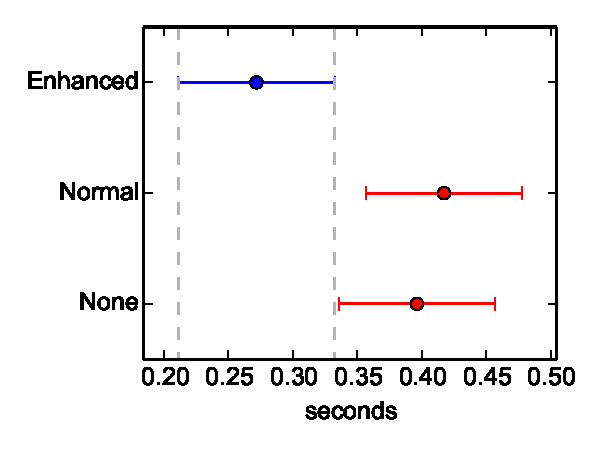
\includegraphics[width=\linewidth]{figs/outpoint-abserr-tukey95.pdf}
  \caption{Tukey's test (95\% confidence interval)}
  \label{fig:outpointerrtukey}
\end{subfigure}
\caption{Absolute error for the outpoint of selections}
\label{fig:outpointerr}
\end{figure}

\paragraph{Zoom}
The experimental interface included two displays -- one overview display
covering the length of the recording, and a zoomed display which showed a
magnified part of that. The number of times the zoom in and zoom out buttons
were pressed was logged. The sum of these values for each visualization is
shown in Figure~\ref{fig:zoomtotal}. By subtracting zoom out from zoom in, we
can infer what the final zoom level was when the response was submitted. The
final zoom levels for each visualization are shown in
Figure~\ref{fig:zoomfinal}.

\begin{figure}[h!]
\centering
\begin{subfigure}{.5\textwidth}
  \centering
  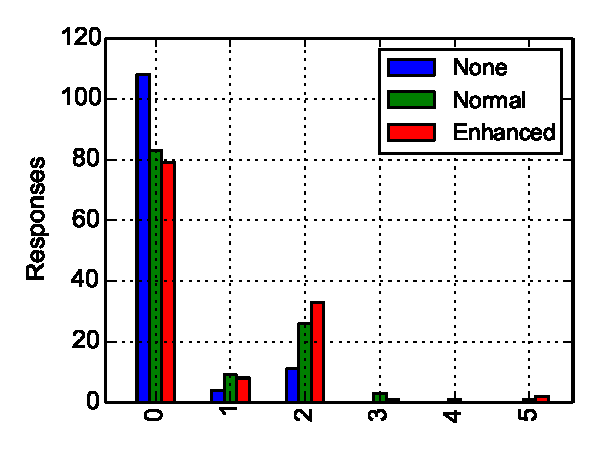
\includegraphics[width=\linewidth]{figs/zoomtotal.pdf}
  \caption{Total zoom actions}
  \label{fig:zoomtotal}
\end{subfigure}%
\begin{subfigure}{.5\textwidth}
  \centering
  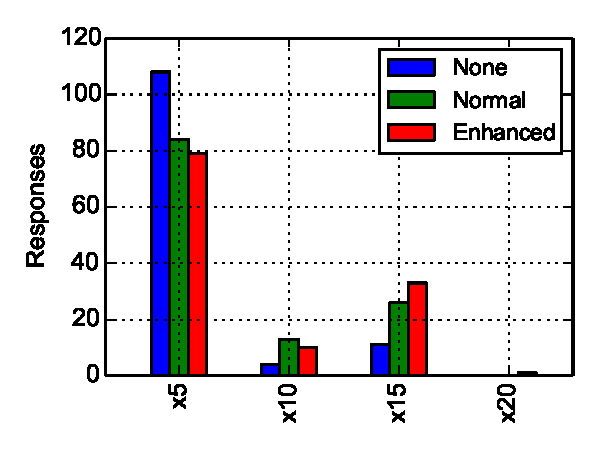
\includegraphics[width=\linewidth]{figs/zoomfinal.pdf}
  \caption{Final zoom level}
  \label{fig:zoomfinal}
\end{subfigure}
\caption{Analysis of zoom usage}
\label{fig:zoom}
\end{figure}

Most of the time, participants didn't touch the zoom controls and opted to leave
it on the default x5 zoom level, which displays roughly one minute of audio
across 1045 pixels ($\sim$50ms per pixel). Other than the x5 level, x15 was
more popular than x10 for all visualizations and x20 was barely used at all.

\subsection{Comparison}
Participants were asked to directly compare the three visualizations at the end
of the experiment. The results are shown in Figure~\ref{fig:compare}.

\begin{figure}[ht]
\centering
\begin{subfigure}{.5\textwidth}
  \centering
  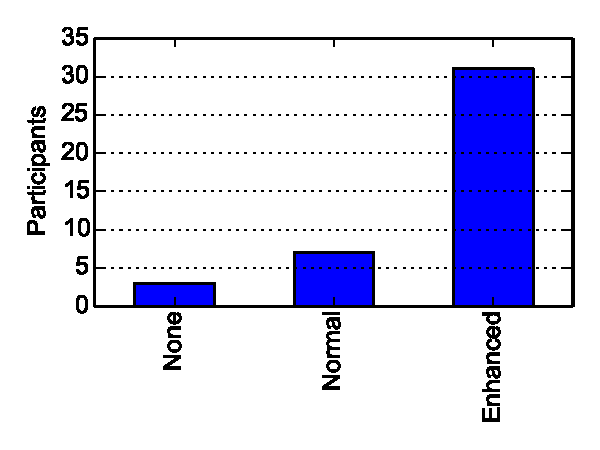
\includegraphics[width=\textwidth]{figs/easiest.pdf}
  \caption{Easiest to use}
  \label{fig:easiest}
\end{subfigure}%
\begin{subfigure}{.5\textwidth}
  \centering
  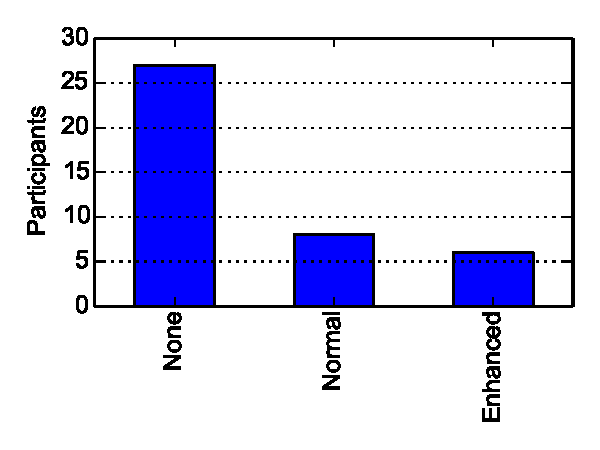
\includegraphics[width=\linewidth]{figs/frustrating.pdf}
  \caption{Most frustrating}
  \label{fig:frustrating}
\end{subfigure}
\caption{Response of participants when asked to compare the visualisations
  using different criteria}
\label{fig:compare}
\end{figure}

A clear majority of 76\% thought that the enhanced waveform was the easiest to
use, with the normal waveform receiving 17\% of votes and 7\% for no waveform.
The strong preference for the enhanced waveform over the others shows that
participants thought the additional information added using colour made their
task easier.

Having no waveform was considered by two-thirds of participants to be the most
frustrating condition, followed by the normal waveform at 20\% and enhanced
waveform at 15\%. Although this is another strong result in favour of using
waveforms, the results are not quite as strong as the ones on ease of
use. It is possible that the false positives and negatives present in the
enhanced waveform caused some people to select it as the most frustrating.

\subsection{Task load index}
The TLX responses were standardised to account for variation in the way
different people assign scores. The distributions of the standardised scores
for each visualization are shown in Figure~\ref{fig:tlx}.

\begin{figure}[p]
  \centering
  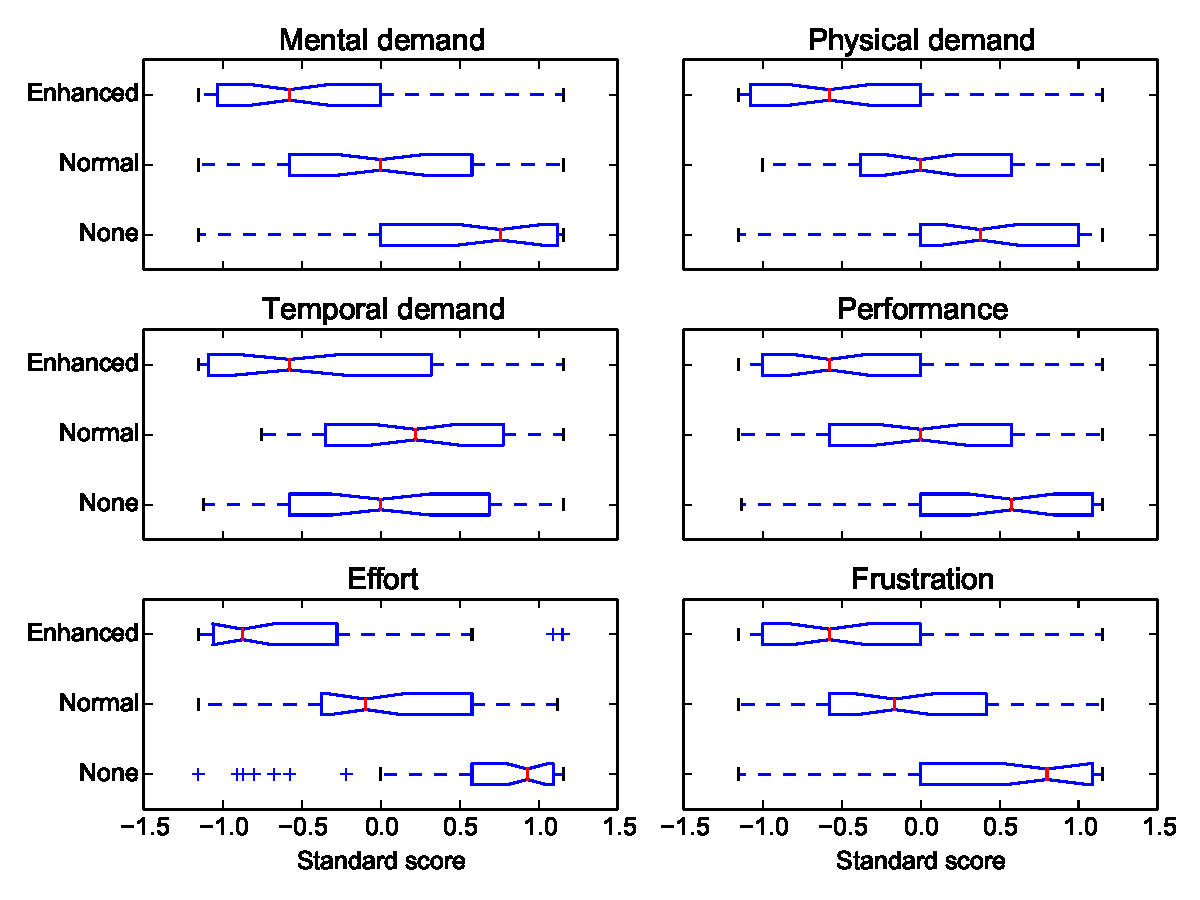
\includegraphics[width=\textwidth]{figs/tlx-std.pdf}
  \caption{Standard score of NASA Task Load Index responses for each
    visualization, standardised per participant.}
  \label{fig:tlx}
\end{figure}

\begin{figure}[p]
  \centering
  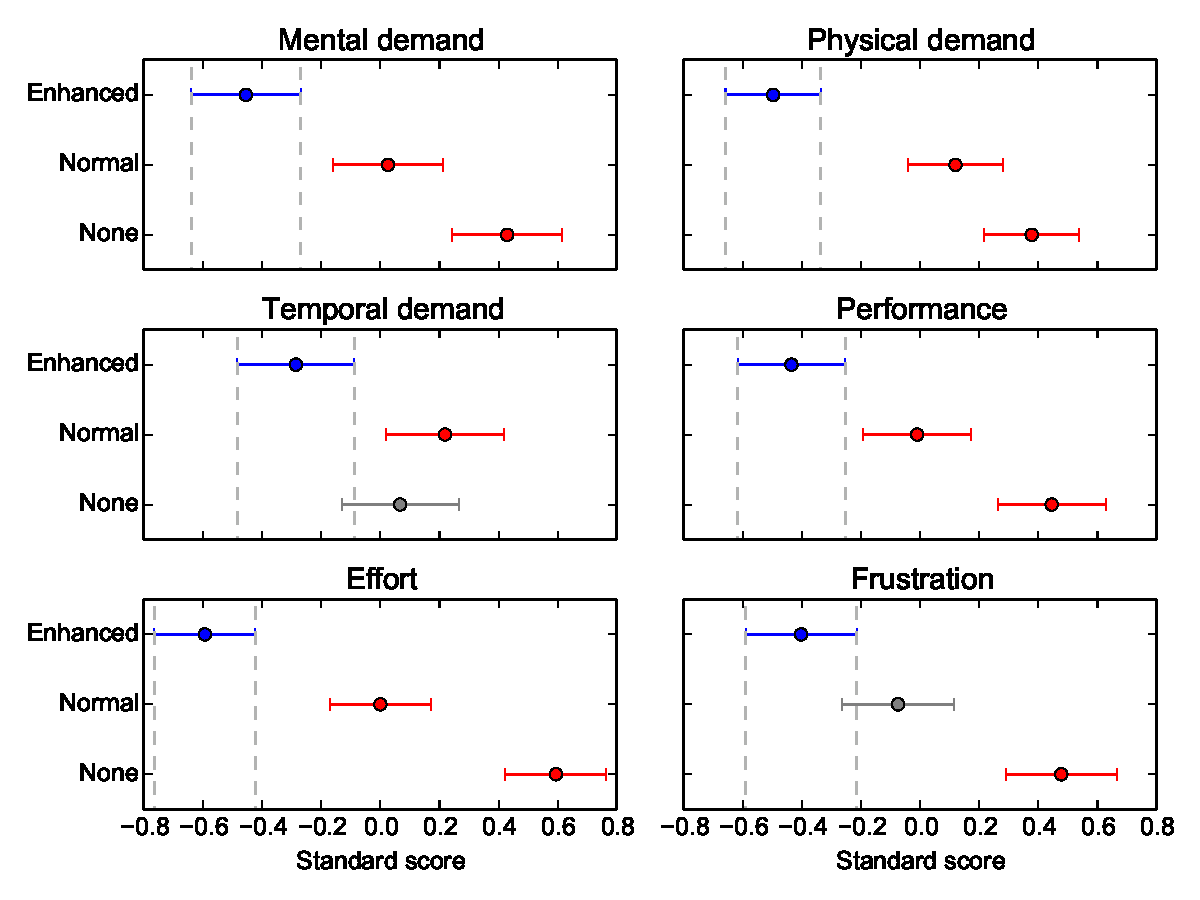
\includegraphics[width=\textwidth]{figs/tlx-std-tukey95.pdf}
  \caption{Standard score of NASA Task Load Index responses for each
    visualization, standardised per participant.}
  \label{fig:tlxtukey}
\end{figure}

ANOVA found there to be significant differences between the visualizations in
all TLX metrics for $p < 0.01$. Tukey's test (see Figure~\ref{fig:tlxtukey})
found that for $p < 0.05$, the enhanced waveform outperformed no waveform in
all metrics except temporal demand, and outperformed the normal waveform in
all metrics except frustration. The normal waveform outperformed no waveform in
mental demand, performance, effort and frustration.

Some scepticism should be given to the physical and temporal demand metrics, as
it's not entirely clear what is meant by that terminology in the context of the
task. Participants are not working against the clock, not are they doing
anything other than moving the mouse. Although some participants may consider
fewer clicks of the mouse to represent reduced physical demand, we cannot
assume that others thought the same.

\subsection{Interaction behaviour}
This section looks at how participants used the features available in the
online audio interface, full described in Section~\ref{sec:iface}.
%Informal observation of some participants as they completed the experiment
%revealed that some people used the interface in different ways. For example,
%when one participant had completed their selection, they scanned through the
%remaining unselected content to check that there were no other pieces of music.

\begin{figure}[p]
\centering
\begin{subfigure}{.5\textwidth}
  \centering
  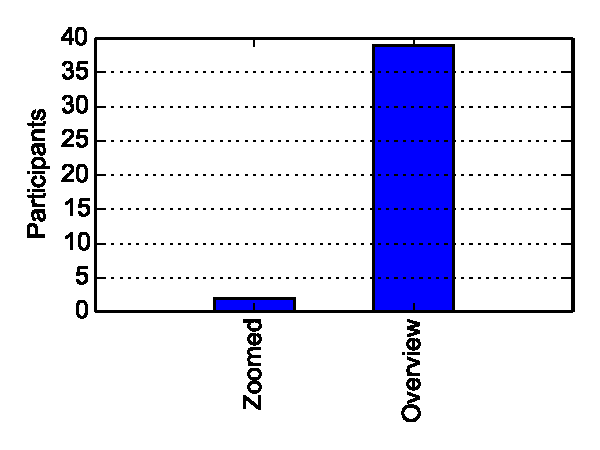
\includegraphics[width=\linewidth]{figs/top-v-bot-pref.pdf}
  \caption{Display}
  \label{fig:displaypref}
\end{subfigure}%
\begin{subfigure}{.5\textwidth}
  \centering
  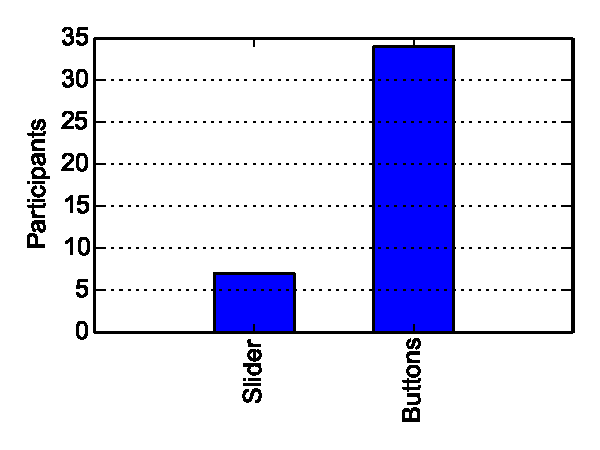
\includegraphics[width=\linewidth]{figs/mark-v-slide-pref.pdf}
  \caption{Selection method}
  \label{fig:selectpref}
\end{subfigure}
\caption{Preference of participants}
\label{fig:pref}
\end{figure}

\paragraph{Top/bottom display}
There are two displays that make up the interface -- a zoomed display at the
top and an overview display on the bottom. Either of the displays can be used
to navigate the recording and make selections.

For each participant, the number of tasks where they used the zoom display more
than the overview (and vice-versa) were counted. Figure~\ref{fig:displaypref}
shows number of participants who, on average, used the zoomed or overview
display more.

The results show a clear preference for using the overview display more than
the zoom display. Coupled with the results of zoom usage in
Section~\ref{sec:studymetrics}, we can see that for this task most people opted
just to work in the overview display, despite only having a resolution of
roughly 300ms per pixel.

An analysis of the overview and zoom display's usage between different
visualization methods did not find any notable difference.

\paragraph{Selection method}
The design of the interface gave participants two methods of making a selection
-- buttons to mark in and out points using the cursor, and a slider where the
in and out points could be dragged around. The cursor can be moved around in
both the overview and zoomed displays, whereas the slider is only available at
the x1 zoom level. This makes the buttons more useful for fine edits, where
high precision is needed. When using the slider, the selection display updates
as you move it making it easier for people to see where their selection is.

For each response, the method with the most actions was found and these
preferences were summed for each participant to calculate their overall
preference. The results are shown in Figure~\ref{fig:selectpref}.

The buttons were the most popular method of making a selection, with only 17\%
of people using the slider more. Informal feedback found that some people has a
strong preference for using the slider but were frustrated that there wasn't a
second slider available on the zoomed display.

\section{Technology development}\label{sec:tech}

\section{Audio visualisation software}\label{sec:vis}
The direction of the research in this project centres around turning audio
data into image data. There is already some software that visualizes audio and
audio features in a number of ways, notably Sonic Visualiser \cite{Cannam2010}.
However, the visualization algorithms are always hard-coded into the program,
making prototyping of new methods prohibitively difficult.

\subsection{Design}
A system of software was developed for visualizing audio in order to allow
flexibility while maintaining consist inputs and outputs. It was
designed to expand on existing systems for audio analysis so to avoid
duplication of effort and to allow modularisation of algorithms.

The system was developed as a plugin framework with clearly defined inputs and
outputs. It is based on the existing Vamp plugin framework, developed by Queen
Mary University of London \cite{Cannam2010}, which analyses audio data and
outputs frame-- or time-based features. The visualization plugin is designed to
take these features and produce a bitmap image. An outline of the system design
is shown in Figure~\ref{fig:vampeyer}.

\begin{figure}[ht]
  \centering
  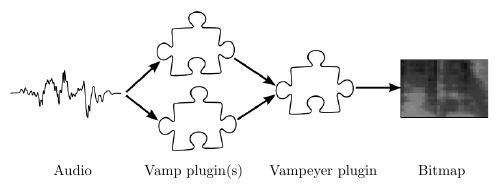
\includegraphics[width=0.8\textwidth]{figs/vampeyer.png}
  \caption{High-level system diagram of the Vampeyer visualization framework}
  \label{fig:vampeyer}
\end{figure}

The visualization plugin defines which Vamp plugin outputs it requires,
including the block/step size and parameters. At least one Vamp plugin is
required, but there is no restriction of the number of different Vamp plugins
that can be used.

Both frameworks are written in C++ which allows for a fast processing time.
This is important for situations where audio has to be processed on-the-fly,
such as for exploring an archive without having to pre-process everything in
it.  The plugins are compiled into shared libraries, so they can easily be
distributed without users having to recompile locally and integrated into
third-party software.

\subsection{Implementation}
A C++ header file was created which implements the design.  Five data
structures are also defined which define how data should be sent and returned
from the functions.

{\singlespacing
\begin{itemize}
  \item \texttt{VampParameter} is a name/value pair used to store a parameter
  \item \texttt{VampParameterList} is a vector of \texttt{VampParameter}s
  \item \texttt{VampPlugin} stores the name of a Vamp plugin along with a
    \texttt{VampParameterList} and the preferred block and step sizes
  \item \texttt{VampOutput} stores a \texttt{VampPlugin} and output name
  \item \texttt{VampOutputList} is a vector of \texttt{VampOutput}s
\end{itemize}
}

Two primary functions are used to define the input audio features and their
conversion to a bitmap.

\begin{itemize}
  \item \texttt{getVampPlugins} returns a \texttt{VampOutputList} variable
    that contains a list of Vamp plugin outputs which must be provided as
    input
  \item \texttt{ARGB} takes the Vamp plugin output data as a
    \texttt{Vamp::FeatureSet} variable, the sample rate of the audio and the
    desired width and height. It returns a bitmap image formatted in 32-bit
    ARGB format (alpha, red, green, blue).
\end{itemize}

A number of example plugins were written to demonstrate the capabilities of
this approach, and to act as useful pieces of software in their own right.
These include a standard waveform, waveform colourised by low energy ratio (see
Section~\ref{sec:studywaveform}), waveform colourised by spectral centroid
(identical to Freesound) and an MFCC grid visualization with waveform overlay.

The plugins need to be run by a host program which reads the audio data,
processes it using the Vamp plugins, sends their output to the visualization
plugin and then writes the image data. Such a program was written as a
command-line tool that can either display the image in a window or write it to
disk as a PNG-encoded file. This makes it useful for both prototyping and for
back-end processing on a server, for example.

\section{Browser-based audio interface}\label{sec:iface}
An audio interface was developed for use in evaluating a number of different
audio visualizations (see Section~\ref{sec:study}). In order to maximise the
number of people who could participate in the experiment, it was designed to be
accessible online and run in a web browser.

The latest web standards (such as HTML5) were exploited in order to ensure a
smooth and consistent user experience. This meant that some people running
older browsers were unable to take part, but the standards are mature enough
that the vast majority of browsers are compatible.

\subsection{Design}\label{sec:interfacedesign}
The screenshot of the  final design of the interface is shown in
Figure~\ref{fig:interface}, which includes of one the training pop-ups.

\begin{figure}[ht]
  \centering
  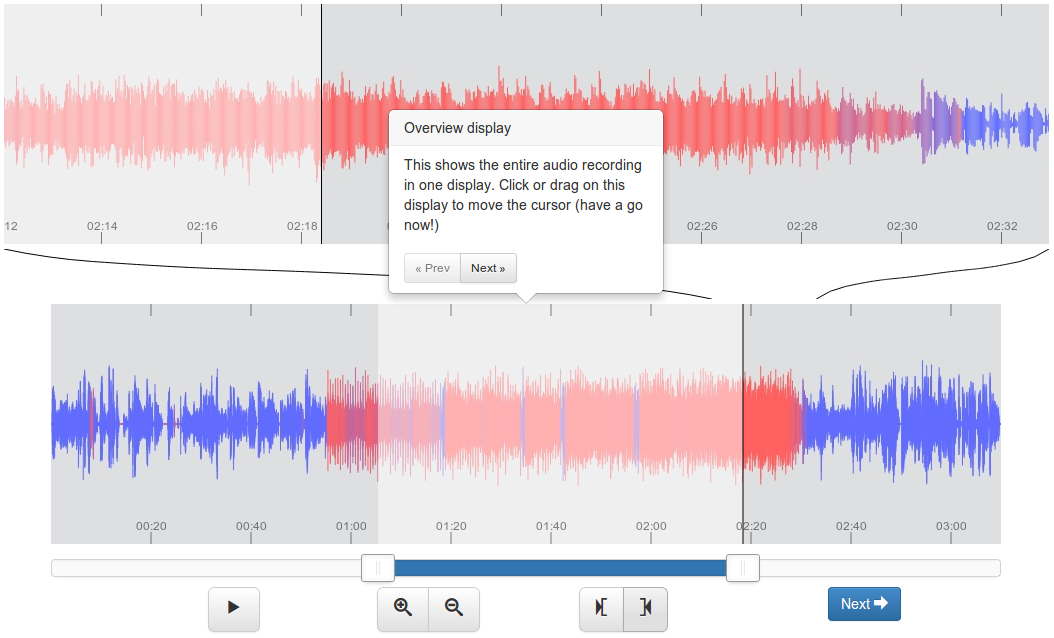
\includegraphics[width=\textwidth]{figs/interface.png}
  \caption{Experimental test interface with training pop-up}
  \label{fig:interface}
\end{figure}

\paragraph{Motivation}
The goal for the design was to include all the essential features required to
complete the task of finding and selecting a segment of audio (see
Section~\ref{sec:studytask}) in a way that can easily be picked up by novice
participants. Only the essential features were considered in order to make it
simple and to avoid distraction.

\paragraph{Displays}
Two displays were used -- one to show an overview of the entire recording, and
another showing an adjustable zoom display. It would be possible to complete
the task using only an adjustable zoom display, but it would be very difficult
to keep track of the position in the recording.

The zoom display was placed above the overview display and set to be slightly
larger than the overview in order to emphasise that the display is a
magnification. The two displays were linked using two curvy lines (splines)
which show the position of the zoom display limits in the overview display.

The current position of the audio playback was signified by adding a `cursor'
using a line on each display. The cursor can be moved by clicking or dragging
on either of the displays using the mouse.

Selected areas of audio are highlighted using a semi-transparent overlay which
appears on both displays.  A time `ruler' was also overlaid on both displays to
give users an objective scale and a sense of the relative scale of the
displays.

\paragraph{Zoom control}
The level of zoom was controlled using two buttons at the bottom -- one to zoom
in and another to zoom out. In an early prototype, users could press these
buttons as many times as they wished, but this caused confusion when maximum
zoom was reached and the button stopped doing anything. Following feedback,
this was rectified by disabling and greying out the buttons when at max/min
zoom.

\paragraph{Selection}
Two methods of selecting content were implemented -- one using buttons and
another using a slider. The buttons were used to set either the in or out point
of the selection to the current position of the cursor. The buttons could be
used while the audio is playing, allowing users to press a button as they hear
their preferred start/end point. As the cursor can be moved on the zoomable
display, the buttons can be used to set the selection precisely.

The slider acts both as a display of where the selection is and as a method of
setting or adjusting it. The slider was located just under the overview display
and has `handles' on each side which can be dragged to adjust the start and end
of the selection. After receiving feedback on a prototype, the slider was
configured to update the highlight in the displays as it is dragged, making
fine adjustments easier to see.

\paragraph{Training}
Although the interface is relatively basic as far as digital audio workstations
are concerned, a system was developed to train users in the features and
operation of the interface. This was done using a `pop-up tour', which is
a technique often found on web pages. It involves a series of dialog boxes
which point out different parts of the interface with some text explaining what
they do. You can see an example in Figure~\ref{fig:interface}.

\subsection{Implementation}

\paragraph{Front-end}
A feature-heavy web page, such one that includes an audio/visual interface, can
be slow to load and unresponsive. To avoid this, the interface was set up as a
`single-page application' which loads the content of each page dynamically
without having to reload the interface and the large Javascript libraries that
it's built on.

Angular.JS\footnote{\url{https://angularjs.org}} is a Javascript web
application framework which aids development of dynamic web pages. A
single-page application was implemented using its `route' and `view' features.
Its other features were used to send responses to the database and update the
cursor/selection on the visualization, amongst other things.

Bootstrap\footnote{\url{http://getbootstrap.com/}} was used to style the page
and the components in it. The popularity of Bootstrap means that this style is
familiar and comfortable to most web users. Bootstrap
Tour\footnote{\url{http://bootstraptour.com/}} is a Javascript library for
running `pop-up tours' on websites. This was used to implement the training
interface, as discussed in Section~\ref{sec:interfacedesign}.

\paragraph{Back-end}
A web server and database were used to serve the web pages and experimental
data, and to store the results. Node.js\footnote{\url{http://nodejs.org/}} was
used to implement and expose an API for interacting with the front-end and
CouchDB\footnote{\url{http://couchdb.apache.org/}} was used as the database.

The sequence for each experiment (described in Section~\ref{sec:studysequence})
needed to be assigned to participants evenly, so that each sequence is
completed exactly once before a second participant is assigned to it. This was
done by taking the sequences that had been completed the least number of times,
then choosing the sequence that had been assigned the longest time ago (or not
at all). This approach minimised the chance of more than one participant using
the same sequence. 

\paragraph{Audio playback}
Different browsers support a variety of different audio codecs and have
different capabilities in terms of playback methods. In order to maximise
compatibility, SoundJS\footnote{\url{http://www.createjs.com/\#!/SoundJS}} was
used to play the audio content.

The audio content was data compressed using a lossy codec to reduce the size
(and therefore loading time) of each web page. Ogg Vorbis was used as the
primary codec, with a quality setting of 2 (approx. 80kbps VBR). For browsers
that didn't support Ogg Vorbis, AAC was used with a variable bitrate of 96kbps.
The use of lossy codecs introduces some audible artefacts. However this is not
part of the experiment and it impacts every audio clip, so is not expected to
bias the results. 

\paragraph{Visualization}
The duration of each of the audio clips used in the experiment is about 5
minutes, and the interface display allows for four levels of zoom. This
produces up to $\sim$2MB of image data which, if loaded at the beginning, would
negatively impact on the loading time of the web page. To fix this, a tiling
system was used where each image was cut into tiles 240 pixels wide. The
displays then dynamically loaded the tiles as and when they were needed.

To ensure maximum browser compatibility and to simplify the implementation,
KineticJS\footnote{\url{http://kineticjs.com/}} was used to render the images,
ruler and cursor.



% !TeX root = main.tex
\chapter{Use of audio editors in radio production}\label{chp:ethno}

\section{Introduction}
The process of creating radio programmes has evolved over nearly a century amid
a rapidly changing technological landscape. Outside of the radio industry, the
production process is not well understood and it can be difficult for those who
want to learn more to gain access. Books \citep{Hausman2012} and studies
\citep{Dunaway2000} on radio production have been written, but as they focus on
editorial concerns, they do not reveal much about practical issues that
producers face.  The lack of available information can make it difficult for
researchers and designers to understand the real-world challenges and needs of
radio production.

Although most radio content is broadcast live, a significant proportion of
programmes, such as documentaries, are created offline using audio editing
software. The audio editing tools used by radio producers are often very basic
in the features they offer and where more advanced software is used, it is
typically designed for production of music rather than speech.

There are many semantic audio and user interface technologies that have the
potential to improve the production environment. Automatic segmentation
algorithms for speech/music discrimination \citep{Wieser2014} and speaker
diarization \citep{AngueraMiro2012} are relatively mature and have already been
applied to radio \citep{Raimond2014}. Experiments into the use of
higher-level representations like text are starting to appear, such as the
video editors from Loviscach \citep{Loviscach2011a} and Hyperaudio
\citep{Boas2011}.  However, without a detailed understanding of the production
workflows, it can be difficult to know which of these technologies have the most
potential, or how they can be integrated into the workflow.

In order to gain a better understanding of the radio production process, a
study was conducted at BBC Radio in London. Section~\ref{sec:method} outlines
the methodology behind the study, Sections~\ref{sec:news}, \ref{sec:drama} and
\ref{sec:doc} present the results of three case studies,
Section~\ref{sec:summary} outlines the results and
Section~\ref{sec:conclusion} presents the conclusions.

\subsection{Production system}
The vast majority of radio production work in the BBC uses a networked audio
production system called \textit{dira!} \citep{SCISYS2015}. It is colloquially
known as `VCS', which is the former name of the company that sells it. All
audio content is kept on distributed storage and the system is accessed using
various pieces of software: `StarTrack' is a multi-track audio editor, `Orion'
is an audio recorder and single-track editor and `Highlander' is used to browse
recordings and metadata. 

\section{Methodology}\label{sec:method}
Previous studies of professional broadcast environments have focused on how
producers collaborate during live production \citep{Engstroem2010,Perry2009}, by
using video recordings to analyse the interactions between producers. The scope
of this study was much wider and covered the production of programmes over a
number of weeks. As such, an ethnographic approach was taken so that all
aspects of the production could be considered.

\subsection{Objective and scope}
The objective of the study was to discover how radio programmes are created, in
order to identify opportunities for assisting or improving the process using
technology. Although the focus was on production tools, the entire production
workflow was considered so that use of tools could be understood in context.

Due to the scale and variety of the radio operations at the BBC, it would be
impossible to cover all production genres and techniques.  Instead, a
representative but varied selection of programmes that use pre-recorded content
were considered. Three case studies were chosen --  a news bulletin, a drama
and a documentary.

\subsection{Data collection}
Information was gathered by observing and interviewing the producers in their
normal work environment. Each team was observed for long enough to gain a full
understanding of each person's role, the environment they work in and each step
of the production process. The observation took between half a day (for the
news bulletin) and four days (for the documentary). The interviews were
unstructured and conducted during `down-time' between observations.  Typed or
hand-written notes were taken throughout the observation and interviews.

Participants were recruited individually by contacting them through a number of
studio managers who had worked with the authors in the past. 

\subsection{Analysis}
The objective of the analysis was to uncover the challenges producers face in
the production process, and to identify how technology can be applied to meet
those challenges.

The information collected from each case study was first categorised into the
producers' roles, the environment they work in and the production workflow from
beginning to end. Challenges and opportunities that emerged from these were
then identified, and potential technology-based solutions were considered.
These were examined to find any strong themes that were common across the
three case studies, or any significant opportunities that resulted from them.

\section{News bulletin}\label{sec:news}
The summaries team at BBC News (known just as ``summaries'') create hourly news
bulletins for the national radio networks\footnote{Except for Radio 1, 1Xtra,
  Asian Network and Radio 5, which are handled by separate teams.}. The team
was observed during a morning weekday shift. The pace of work in the team is
extremely fast so most of the observation was passive.

\subsection{Roles}\label{sec:news-roles}
Summaries is run by an \textit{assistant editor} who leads a number of
\textit{broadcast journalists}. The team work on rolling shifts to help keep
track of developing news stories. The role of each journalist is to select and
write short text summaries of news stories for a particular network. They must
find and edit audio clips to accompany those stories and construct them into a
bulletin of a set length.  The assistant editor performs the same role as the
journalists, but is also responsible for assigning the bulletins to the team,
deciding which stories to prioritise, and to read and approve each news
bulletin. The finished bulletins are read out live by a \textit{presenter} in a
radio studio.

Summaries work closely with other news teams to gather audio content. The
`\textit{intake}' team set up and record live incoming feeds from
\textit{reporters} in the field. They notify summaries of the incoming feeds so
that they can listen-in and provide instant feedback. The `\textit{newswire}'
team provide curated clips of both BBC and user-generated content. Summaries
also work with individual \textit{reporters} who are commissioned to record
clips for the bulletins. These are recorded and edited by the reporters
themselves and provided to the team directly.

\subsection{Environment}
The team sit together at a large desk in the BBC newsroom (see
Figure~\ref{fig:newsroom}), which also houses teams from around the BBC News
division.  The working environment is configured to facilitate fast flow of
communication, which is reflected in the design of the newsroom and the
equipment on the desks.  Each space at the desk has a PC, telephone, intercom,
TV monitor and headphones. The intercom is used to communicate with other teams
in the newsroom, and the TV monitor displays the BBC News channel. However by
design, most communication is face-to-face.

\begin{figure}[ht]
  \centering
  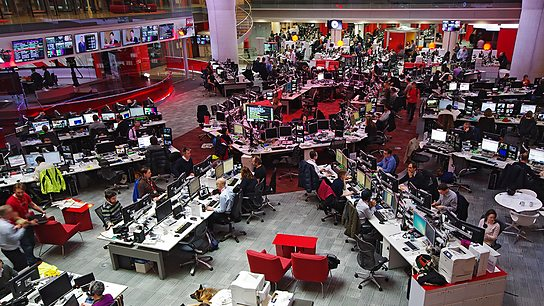
\includegraphics[width=\columnwidth]{figs/newsroom.jpg}
  \caption{The newsroom in BBC New Broadcasting House.}
  \label{fig:newsroom}
\end{figure}

Most of the work is based at a desktop PC and primarily done on the Electronic
News Production System (ENPS). This is an industry standard software package
for writing scripts and compiling news bulletins. It integrates with the
\textit{dira!} radio production system using a plugin called Media Object
Server (MOS). This allows users to browse and edit audio clips within ENPS (see
Section~\ref{sec:news-clips}).

\subsection{Workflow}
Each journalist produces one bulletin per hour, each between two and five
minutes long, depending on the network and the time of day (e.g. midday
bulletins are longer). Even if the stories being covered are the same, the
bulletins for each network are written separately so that they suit that
network's audience. This is done by varying the number of items, the amount of
detail and the level of assumed knowledge. The team aims to finish bulletins 15
mins before they are aired.

\subsubsection{Scripts}
Using ENPS, the team write text summaries of the current big news stories and
compile them into a bulletin. The information comes from a variety of sources,
but mainly from the news wires (e.g. Reuters) and BBC reporters.  The finished
bulletin must fit an exact time slot, so much of the work and skill is in
knowing how long the text will take to read and being able to condense the
story down to the key points. 

\subsubsection{Audio clips}\label{sec:news-clips}
Each bulletin contains a number of audio clips which help to break up the
newsreader's voice and make the piece more engaging.  Relevant audio content is
selected, edited to an appropriate length and inserted into the news script.
All clips are stored in \textit{dira!} and the MOS plugin is used to find, edit
and insert the clips into ENPS (see Figure~\ref{fig:news-enps-edit}).  This
uses \textit{dira!} Orion which offers basic cutting, levels and fading
functionality. When a clip is finished, it is dragged onto the script at the
point in the text where it should be played. The user must give the clip a
name, and can optionally add the in and out words\footnote{The 2/3 words spoken
  at the beginning and end of the recording.}. These and the clip duration
appear in the script which helps the journalists and newsreader.

\begin{figure}[ht]
  \centering
  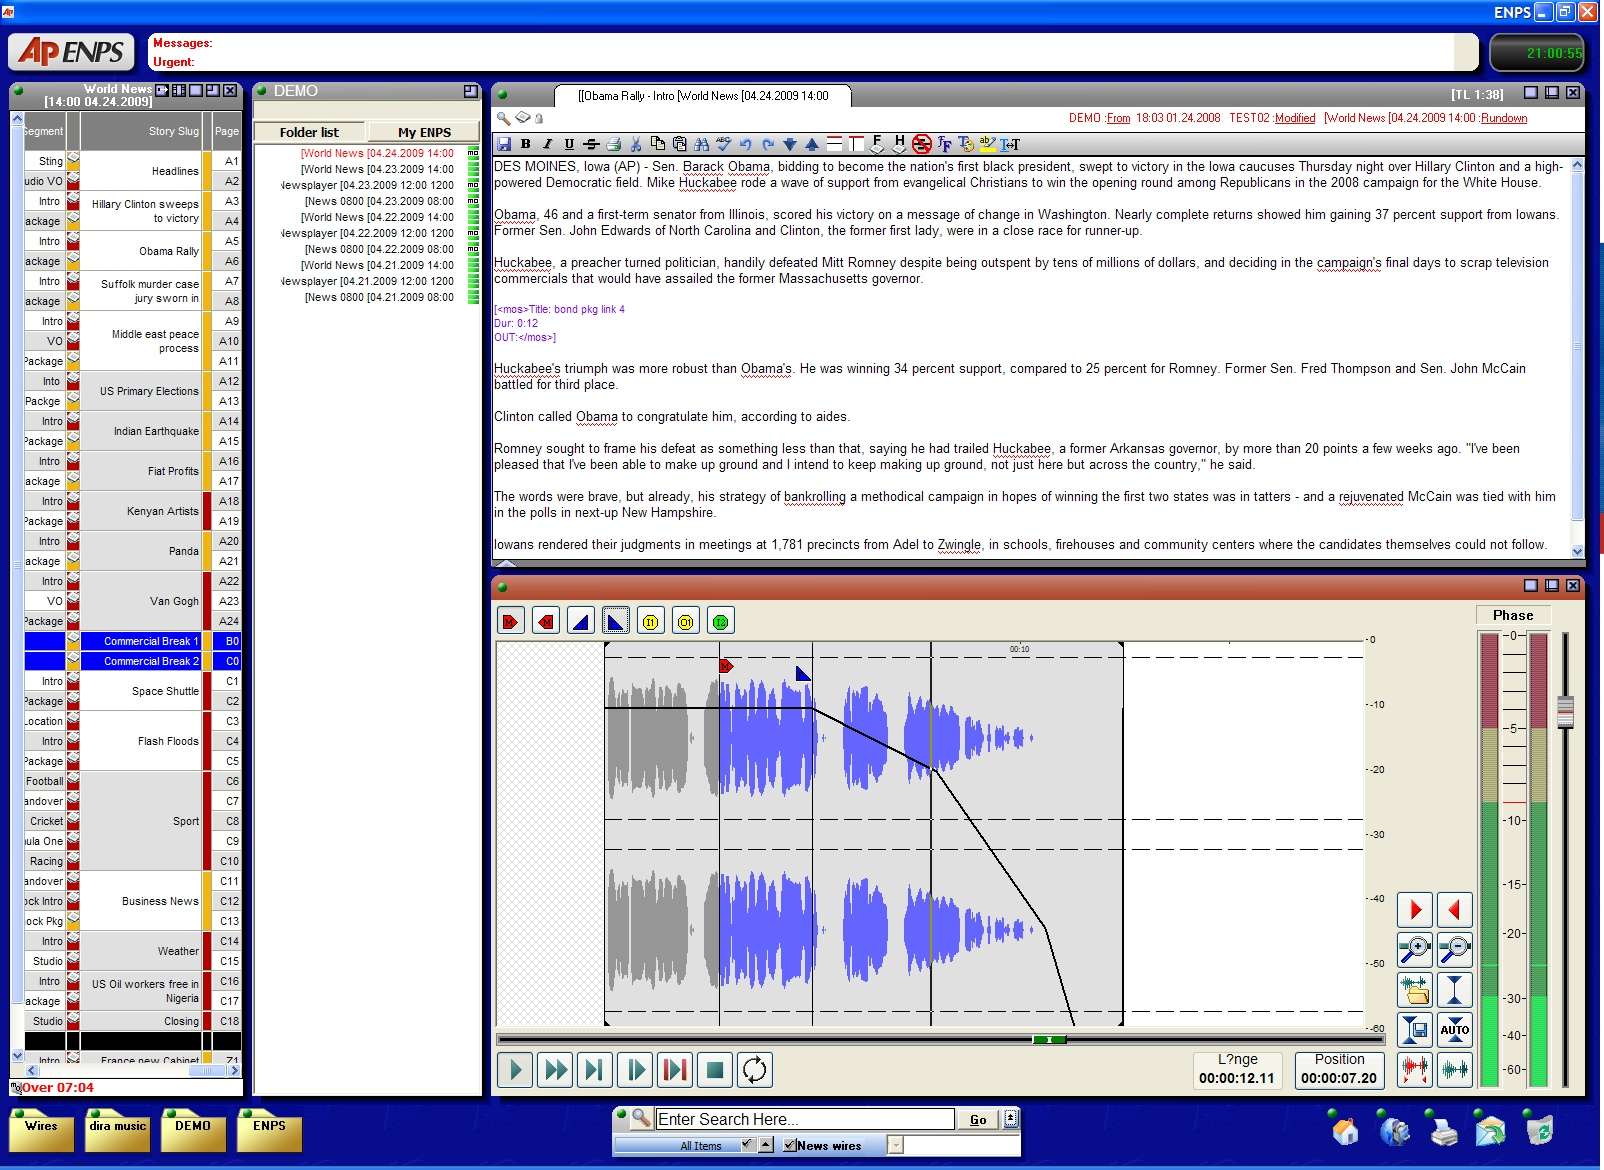
\includegraphics[width=\columnwidth]{figs/news-enps-edit.jpg}
  \caption{Editing a clip in ENPS using the MOS plugin for \textit{dira!}.}
  \label{fig:news-enps-edit}
\end{figure}

Audio content comes from a variety of sources including the intake team,
newswire team, and individual reporters (see Section~\ref{sec:news-roles}).
Off-air content from the BBC News TV channel is also used.  For off-air
recordings, the journalists must find and clip the audio themselves. Sound from
the TV channel is automatically recorded into \textit{dira!} in 40-minute
chunks. The recordings are navigated using the MOS plugin, which only displays
a waveform and timeline. Without knowing what time the clip starts, the
journalists resort to skipping through the 40 minutes listening out for a
familiar voice or word, which can be time-consuming and frustrating.

\subsubsection{Playout}
When a journalist has finished the scripts for their bulletin, these are placed
into a `running order' which is named with the network and time (e.g. `R4 Thu
10:00'). The assistant editor then reviews the scripts and listens to the clips
to ensure they comply with editorial policy and use the correct language and 
pronunciation.  Any required changes are made by the journalist or
editor before they are marked as approved. This gives the scripts a green label
in ENPS which indicates that they can be read on-air.

The presenter sits in a radio studio and normally has no direct contact with
the summaries team. At the time of the news bulletin, the presenter reads the
news scripts from ENPS live on-air. The audio clips in each script are
automatically loaded into the playout system, and the presenter triggers them
at the correct time.

\subsection{Challenges and opportunities}
Finding and cutting clips out of long recordings is a particular challenge.
There is very little information to go on so users resort to seeking through
the recording, listening out for someone's voice or mention of a certain topic.
The pressure of a fast turn-around makes the situation even more frustrating.
Application of segmentation or speech-to-text technology could help by
indicating where people are speaking, displaying keywords that are mentioned,
or allowing the recording to be searched by text.

When it comes to inserting clips into the script, in and out words are manually
entered so that the clip can be recognised, but there is not enough time to
transcribe the whole clip. Speech-to-text technology would be able to automate
this and full transcription could further help the journalists to recall the
clip and write the script around it.

\section{Drama}\label{sec:drama}
Radio 4's ``15 Minute Drama'' is a series of original drama and book
dramatisations, broadcast twice-daily. Production of radio drama is radically
different from that of news as it is based on a script of a radio play and is
created over a number of weeks.

\subsection{Roles}
The production team is made up of five members, plus a cast of actors. The
\textit{director} is the owner of the programme and works with the team to
create their interpretation of the radio play. The \textit{broadcast assistant}
handles the administrative side and during the recording, they annotate the
script with detailed notes. There are three \textit{studio managers} (SMs). The
\textit{panel SM} leads the recording process and operates the mixing desk.
The \textit{grams SM}\footnote{`Grams' refers to gramophones, originally the
  only way to play back sound effects.} makes the recordings and plays
pre-recorded sound effects.  The \textit{spot SM} works in the studio where
they place microphones and create spot effects\footnote{Known as `foley' in the
  movie industry.}.

\subsection{Environment}
The observed drama was recorded in studio 60A, which is a purpose-built
flexible performance space at BBC New Broadcasting House in London. It contains 
spaces with different acoustic properties including movable absorbers and a
foam-lined spiral corridor, used to simulate distance. There are many fixtures
and props for re-creating common environmental sounds including various
doors/windows, a staircase with both wood and carpet, a bedroom and a working
kitchen.

The studio is connected by a large acoustically-isolated window to the cubicle
where the production team sit (see Figure~\ref{fig:drama-studio}). The mixing
desk is in front of the window with the broadcast assistant to the right and
the director behind. The grams SM sits at the back of the room, while the spot
SM spends most of their time in the studio.

Post-production is done in an editing suite which is a compact
acoustically-treated room with a PC, speakers, small mixing desk and level
meters.

\begin{figure}[ht]
  \centering
  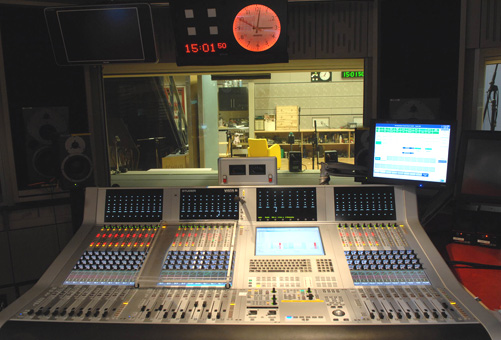
\includegraphics[width=\columnwidth]{figs/60a.jpg}
  \caption{Cubicle of studio 60A.}
  \label{fig:drama-studio}
\end{figure}

\subsection{Workflow}
Prior to the recording, the cast will have done a read-through where the
broadcast assistant notes the time taken to perform each scene.

\subsubsection{Recording}
The whole team is present during recordings and they normally record at least
one episode in a day. The scenes are done in sequence, with multiple takes
recorded for each. When the director is satisfied with the takes, the recording
moves onto the next scene.

During the recording, the panel SM balances the microphone feeds and sound
effects, and makes a backup recording onto a CD. The grams SM records the desk
output directly into a digital audio workstation (DAW) and stores each take as
a separate clip. The DAW is used to manually label each clip with the episode,
scene and take number (e.g. e2s3t1). The grams SM also selects and plays
environmental recordings and sound effects, which are recorded onto a separate
track in the DAW. The spot SM positions the microphones for the actors and
creates live spot effects in the studio. The director listens carefully to the
takes and makes their own notes.  Between takes, they discuss the performance
with the team and give feedback to the actors.

The broadcast assistant takes detailed notes throughout the recording by
annotating a paper copy of the script and keeping a spreadsheet of the takes
and their length. The paper annotations (see Figure~\ref{fig:drama-script})
have a well-defined syntax which is explained below. Although this syntax is
widely used, it is not formally defined so can vary from person-to-person.

A different coloured pen is used for each take. The start and end of each take
is marked with a vertical line on the side of the page, with the take and
backup CD numbers written at the top. If the take is repeated within a 
recording, the line continues back to the top. Repeated words or phrases are
marked with square brackets. If multiple brackets overlap, their order is
labelled with numbers.  Words that are spoken incorrectly are underlined. The
best take for each scene is marked by using highlighter pen on the vertical
line for that take.

\begin{figure}[p]
  \centering
  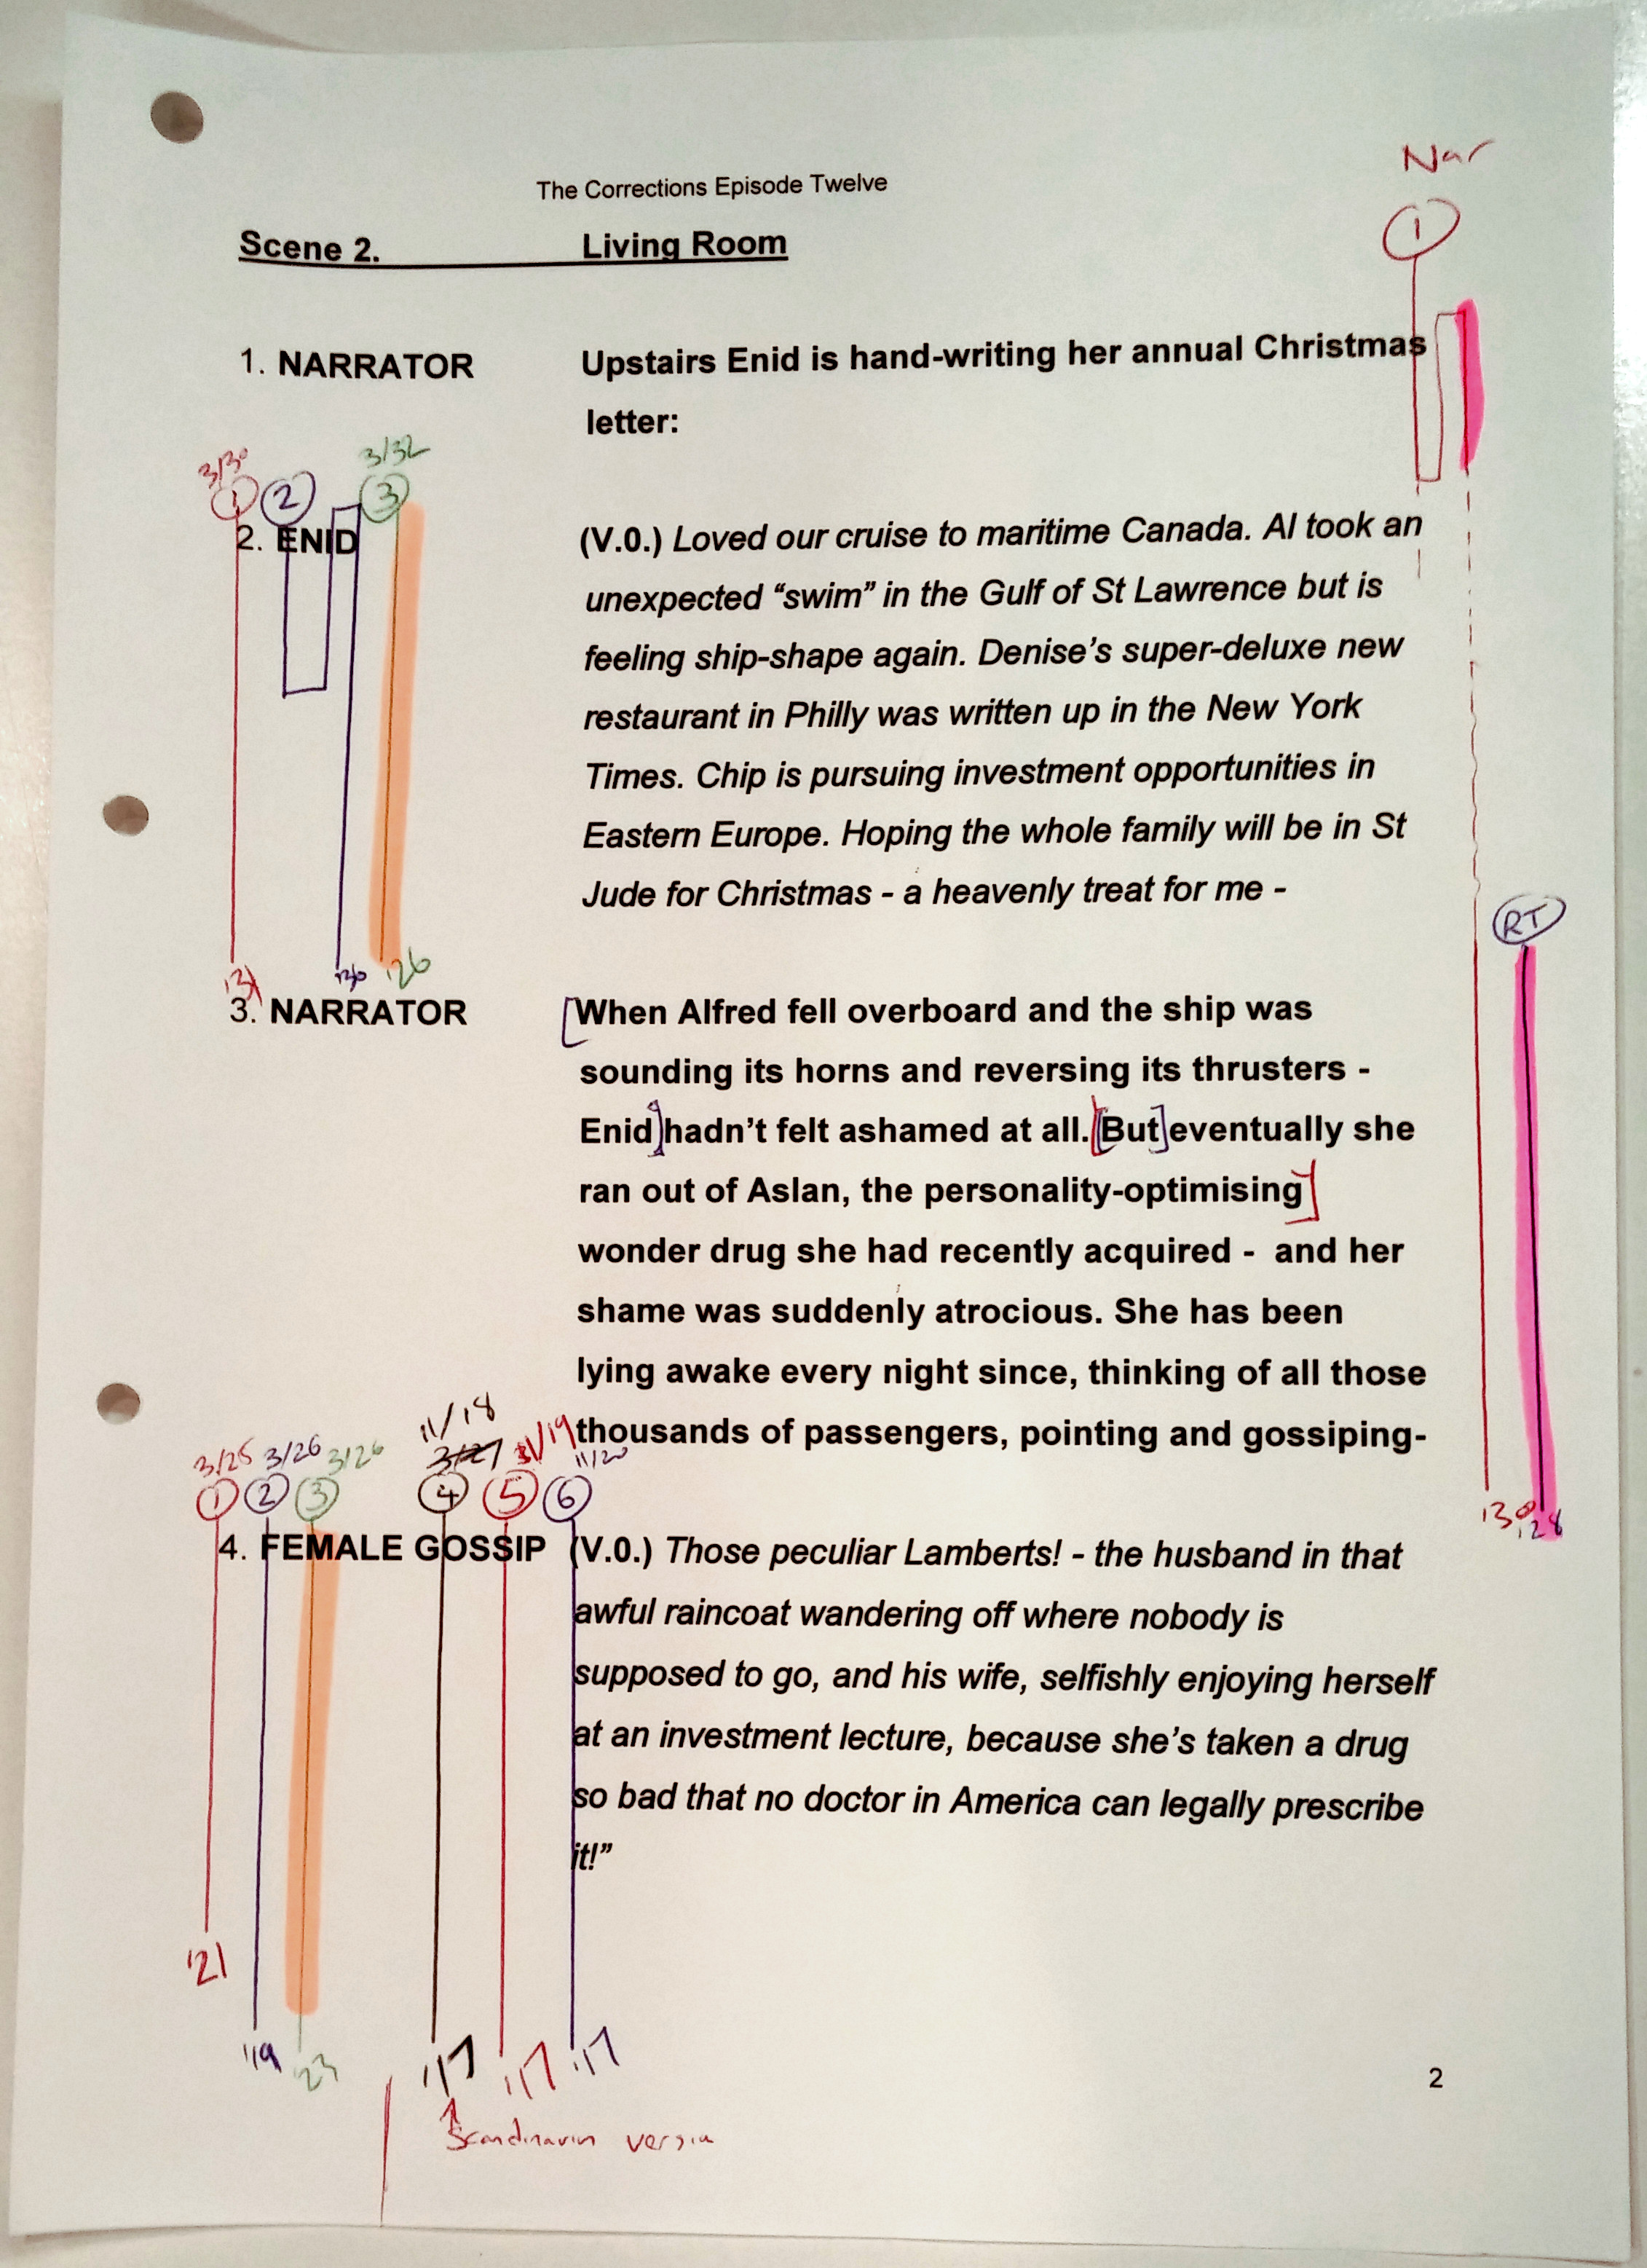
\includegraphics[width=\columnwidth]{figs/drama-script-example-processed.jpg}
  \caption{An annotated drama script page.}
  \label{fig:drama-script}
\end{figure}

After the recording is complete, the audio files are copied onto a portable
hard drive. Although hard drives can fail and be misplaced, they are still used
as the computer network is considered too slow and the hard drive can be taken
anywhere.

\subsubsection{Rough edit}
The rough edit is created with a DAW by one of the studio managers, usually the
panel SM. As the files are stored on a portable hard drive, this process can be
done either in an edit suite or on a laptop at home. The first step is to
create a sequence of the best takes from the recordings. The annotated script
is used to identify these, and they are dragged from the DAW's `clip list' onto
a timeline. There can be many clips, so sometimes they are searched with text
to narrow-down the list. Mislabelled clips or misread labels can occasionally
cause issues at this stage.

The script is used to identify and remove errors in the takes, particularly
re-takes or repeated words. Sometimes these are missed and must be removed
later. The sound level is adjusted to be consistent throughout, either by using
the mouse for in/out fades or by recording automation with a mixing desk
slider.

Sound effects that are listed in the script but were not played at the time of
recording are added at this stage. Roughly 600GB of effects are stored on the
local computer and their metadata can be searched using text. It takes skill
and experience to know which words to use for the search or to know which CDs
or collections to use for certain effects.

The recordings are listened to so that any unmarked errors are identified, such
as noise caused by actors handling the script during recording. Long sequences
are played at double-speed to save time.

\subsubsection{Fine edit}\label{sec:drama-fine}
Once the rough edit is complete, the director joins the SM in an edit suite to
cut the programme to the correct length, select the best performances, tweak
the sound effects and add background music.

The finished programme must have an exact duration to fill its assigned
broadcast slot. Almost always, the programme will be too long and some lines
must be removed. This can only be done by the director as these decisions have
a strong editorial impact.

While listening through the programme, the director may want to compare the
chosen take with other takes that were recorded. To do this, the SM must find
the correct recording using their labels, drag it onto the timeline and find
the right position in the recording. This process introduces an overhead which
can put directors off comparing performances too often.

Music is not specified in the script, so the director has the creative freedom
to choose what they want. Popular consumer music services are used to find
commercial tracks, but often directors will choose `production music', which is
designed for TV/radio and is easier to license. These are found using one of a
number of online music libraries which, similarly to the sound effects, are
searchable using descriptive keywords. The director provides the music to the
SM on a USB storage device for them to insert and mix.

Once finished, the final edit is mixed down to stereo by playing the programme
through a digital loop-back. Although this can be done automatically, it forces
the director and SM to listen to the programme from beginning to end in one
go.

\subsection{Challenges and opportunities}
The clear syntax used to annotate the drama script shows that the production
workflow is well-organised and makes good use of existing tools. However in the
rough edit stage, the SM is performing simple non-creative editing tasks based
purely on the annotations. If these could be captured in a digital format, the
rough edit stage could conceivably be fully or partly automated.

In addition to being script-based, a defining characteristic of drama
production is that multiple takes are recorded in order to capture the best
possible performance. However, there is no simple way to directly compare
performances so the director relies heavily on the script annotations and
written notes. Providing an easy method of comparing different takes by ear
could potentially lead to selection of better performances.

When actors fluff a line, they often say the line again immediately which is
usually noted in the script with square brackets. However, these can be missed
and are not easy to spot in a DAW. Simple audio analysis could be used to
detect and highlight where this happens.

\section{Documentary}\label{sec:doc}
``The Report'' is a weekly investigative documentary that covers topical news
stories. It is produced over a three week period by the BBC Current Affairs
team and is broadcast at 8pm every Thursday on Radio 4. The team was observed
for four days at various points during the three weeks.

\subsection{Roles}
The documentary is created by a core team of three people. The
\textit{producer} owns the programme. They decide what the story-line will be,
who to interview and how it is edited. The \textit{researcher} assists
the producer with research and investigation, setting up interviews and
transcribing recordings.  Both work full-time on the documentary throughout
the three weeks.  The \textit{presenter} is the narrator for the documentary.
The Report has a regular presenter who typically works on two or three
documentaries at once.

The team is supported by the \textit{editor} who runs the current affairs team.
They provide feedback on the documentary and must give approval for the
documentary to be broadcast. On the final day of production, a \textit{studio
  manager} (SM) joins the team to create the final edit.

\subsection{Environment}
The team is based in BBC New Broadcasting House in London. Their desks are
grouped together in an open-plan office, beside four studios. The studios are
organised into pairs so that one can be used for recordings and the other as a
control room. Each studio is acoustically treated and contains a PC, mixing
desk, microphones and a telephone.

\subsection{Workflow}
The three weeks it takes to create the programme can be very roughly divided
into research, interviews and editing. However in reality these activities
are dependent on external factors and can overlap significantly.

\subsubsection{Research}
The purpose of the research stage is to take the idea behind the programme and
form an interesting and relevant storyline around it. Often the topic will be
in the news that week, so the producer will be looking for an interesting angle
which can be explored in greater depth.

The research stage does not require any special tools other than a web browser
and a telephone. The team will read around the topic so that they are
knowledgeable enough to tell the story well and can identify a number of
people they want to interview. Popular sources of information are previous
reports or documentaries, newspaper articles, encyclopedias and contacts who
already know the subject. The producer will make rough notes for themselves in
Microsoft Word and prepare a draft outline of the programme.

\subsubsection{Interviews}
Once the team have identified who they would like to interview, they will
approach them to see if they are interested. If the interviewee has the time
available, the producer or researcher will do a `pre-interview' over the phone
to see what the person will say and whether it fits the documentary.

Most interviews are done face-to-face, either on-location or in a studio,
depending on the situation. A portable audio recorder and shotgun mic is used
for recordings outside of the studio. The presenter holds the microphone and
asks the questions while the producer controls the recorder and the microphone
level. Recordings in the studio are made straight into the \textit{dira!}
system using Orion.

If it's not possible to meet face-to-face, interviews can either be done using
a local studio and ISDN\footnote{Integrated Services Digital Network.  A
  communication standard that can be used to send low-latency digital audio
  over telephone networks.} link, over the phone but with a portable recorder
at each end\footnote{Known in the business as a `simulrec' or `mic hold'.},
using an IP-based link such as Skype, or just over the phone. The phone is
always a last resort as the quality is very poor.

\subsubsection{Rough edit}
When a producer is working on their own, they will usually edit the interviews
directly using a DAW. However, when a team is collaborating with 
interview material, all of the recordings are first transcribed. Some of
this is done using a third-party transcription service, but the programme's
budget can only cover transcription of three or four interviews. The rest must
be transcribed by the team themselves using Microsoft Word. Whereas the
professional transcription service includes every word, the team's own
transcriptions will skip out many words, leaving only enough to get a good idea
of what they said.

The transcriptions are printed out on paper and the team works with these
printouts until the last few days of production. Lines from the interviews that
they want to use in the programme are marked with highlighter pen. Other
informal notes are made on the paper.

The producer takes the annotated transcriptions and pieces together a rough
edit using \textit{dira!} StarTrack. As the position of each question in the
transcription is marked with a timestamp, the producer can narrow-down the
location of the highlighted text in the recording, but only to within a few
minutes. For each interview, the producer cuts out and saves any lines that
they have highlighted. These are then sequenced into a rough edit of the
programme.

While the producer creates the rough edit, the presenter writes the programme's
`links' -- the narrative elements that join the interview clips. When the first
rough edit is complete, the whole team sits down with the editor for a
`run-through'. The programme is performed out loud, straight-through from
beginning to end, with the presenter reading the links and the producer playing
the clips. This allows the editor to hear the programme and give feedback early
on, and for the length of the current edit to be determined. This run-through
process typically happens two or three times for each programme.

\subsubsection{Fine edit}
The fine edit happens on the day that the programme is to be broadcast. A
studio manager (SM) joins the team to create the final mix. The fine editing
requires that the rough edit is transferred into a DAW that has more features
than \textit{dira!} StarTrack.

The SM starts by cleaning up the interview clips. This is done by removing
redundant noises (e.g. `umm') and phrases (e.g. `you know'). Some are left in
as they are too difficult to remove or are editorially relevant. Long pauses
are removed to ensure there is a good pace, but are sometimes left in for
effect.  The SM also balances the levels by recording automation using a fader
or by dragging in/out fades. 

The links are recorded by the presenter who sits in the studio opposite the SM.
This is done straight into the DAW and the intro/outro to each clip is played
to the presenter. The producer sits in and gives feedback to the presenter over
an intercom. After the links are recorded, the SM goes back to correctly align
the interview and link clips in the timeline.

The Report has theme music which is added at this stage, along with any
additional music chosen by the producer. Similarly to drama (see
Section~\ref{sec:drama-fine}), production music is often used and is chosen
using an online library.

Once all of the elements have come together, the producer and SM must cut the
programme down to a specific duration (in this case 27:45). This is done by
removing sections of speech that can be cut without impacting on the story.
These are usually found at the beginning and end of interview clips.

The finished programme is played for the editor who gives their final feedback
and approval.  Once signed-off, the documentary is mixed down to a stereo .wav
file and imported into \textit{dira!}. The producer must then listen to the
entire programme in \textit{dira!} to ensure the bit-stream that will be
broadcast contains no errors.

\subsection{Challenges and opportunities}
The documentary production relies heavily on paper-based transcripts. This
allows the team to easily collaborate and to make notes, but means that there
is a disconnect between the words and audio content. This results in wasted
time when the producer has to go back and cut out the selected parts of the
interviews. There is also no easy way to listen back to a line in the
transcript. Creating a link between the transcripts and the audio recordings
would allow the producers to work with transcripts as normal, but to
simultaneously navigate and edit the audio content.

The fine edit revealed opportunities for assisting the studio manager with the
clean-up process. If an acoustic model of redundant noises and phrases was 
developed, these could either be highlighted, cut for easy removal or removed
automatically.

\section{Findings}\label{sec:summary}
Generally speaking, the study identified a number of opportunities to improve
the handling, generation and presentation of metadata, as discussed below.

\subsection{Text-based working}
The study found that the production teams relied strongly on scripts and
transcripts of the audio content. The rough edits for both the drama and
documentary were directly created from annotated scripts of the recordings.
Additionally, the news summaries team manually annotate their audio clips with
in/out words to help them identify the recordings. These workflows indicates
that producers would much rather work with text representations than with audio
on a timeline.

Creating a link between the words in the transcript and their position in the
audio could allow the producers to navigate and edit with text as they prefer,
but for the audio to be edited automatically. Hyperaudio \citep{Boas2012} is an
example of a web-based video editor that already uses this approach. In the
case of dramas and documentaries, the full text of the recordings is already
available so speech alignment technology such as SailAlign
\citep{Katsamanis2011} could be used instead of full speech-to-text.

\subsection{Use of paper}
Both the drama and documentary teams preferred to work with paper copies of the
scripts. Many producers are not technology-savvy and are therefore much more
comfortable with the idea of paper. It also affords them the freedom to make
unstructured notes and easily collaborate face-to-face. However, the use of
paper also creates a barrier between the work done on the page and the work
done on the screen. Digital pens and interactive paper are tools that have the
potential to break that barrier while retaining the advantages of both ways of
working. Further investigation is needed to see how such a system could
integrate the two approaches and whether the technology is viable.

\subsection{Redundant speech}
Observation of the fine edit in the documentary found that a significant
proportion of the studio manager's time was spent on cleaning-up interview
material. Much of this was caused by redundant noises such as `umm's and
`err's, or redundant phrases like `you know'. These could be identified using a
system designed or trained for the purpose.  Depending on the producer's
confidence in the algorithm, it could either remove the redundant material
automatically or assist the studio manager in identifying and removing the
material. 

\subsection{Speaker diarization}
All of the observed productions could benefit from being able to see where
different people are speaking in a recording, known as `speaker
diarization'. In drama it would help the producers identify different lines in
the script, in documentaries it would highlight the position of the questions
in interview recordings, and in news it would help producers find what they're
looking for more quickly in long off-air recordings. The research around
diarization is fairly mature \citep{AngueraMiro2012} and although it is starting
to be used in some experimental BBC services such as the World Service Archive
\citep{Raimond2014}, it has yet to become available any mainstream production
tools.

\subsection{Comparing takes}
Drama production is unique in the way it records multiple takes of the same
content. This technique allows the producers to get the most from the actors,
but means that it can be difficult to select which performances to use.
Comparing takes during post-production is possible but the process is clumsy.
Providing an easy way to directly compare performances would allow the director
to make a better informed decision on which to use. If the rough edit for the
drama was assembled automatically, comparison could be made easier by aligning
the takes on different tracks.

\section{Conclusion}\label{sec:conclusion}
An ethnographic study of radio production was conducted by exploring three case
studies. It found that producers of speech radio prefer to work with text-based
representations of audio rather than with the recordings directly. Their
workflows are primarily paper-based which creates extra work when moving
between paper and audio. Creating a link between the words on the paper and
their location in the audio recordings could significantly improve the
production workflow.

The study also identified opportunities to apply semantic audio technology and
interaction design to radio production tasks. Lots of time is spent cleaning up
recordings by removing redundant speech, which could be fully or
semi-automated. Segmenting speech content by speaker would make a positive
impact on most speech-based tasks. Finally, drama productions could benefit
from an easy way to compare multiple takes of the same scenes.


\chapter{Screen-based semantic speech editing}

\section{Introduction}
Speech is a natural form of communication which is rich in information. Since
the early twentieth century, radio broadcasting has been used to transmit and
consume speech-based content. Today, radio listenership remains high and
podcasting continues to grow in popularity. 

Although many radio programmes are still broadcast live, a large proportion are
pre-recorded and put together using audio editing software. Efficient
navigation and editing of speech is crucial to the radio production process.
However, unlike text, speech must be consumed sequentially, and does not
naturally support visual search techniques \citep{Wolfe2004}. 

Audio editing interfaces display a visual representation of the amplitude of
the sound, called a `waveform'. This gives users some ability to visually
search and scan audio content. Although the waveform is useful for many editing
tasks, it displays very limited information, especially when zoomed out
\citep{Loviscach2011}.

Semantic audio analysis technology can be used to extract higher-level
information from the sound, such as whether it is speech or music
\citep{Panagiotakis2005}, where different people are speaking
\citep{AngueraMiro2012} or an approximate transcript of what they are saying.
Presenting this information to the user could allow them to navigate and edit
audio content much more efficiently \citep{Whittaker2004}.

In this paper, we investigate semantic speech editing in the context of
professional radio production. We explore what the typical production process
is, including the workflow and tools that are used. Based on our
analysis, we then introduce a semantic audio editing system that automatically
transcribes speech recordings, and allows users to navigate and edit the speech
using the text of the transcript.  We evaluate the resulting system though a
qualitative study of professional BBC radio producers who use our semantic
editor to create real radio programmes for broadcast.

% RESEARCH QUESTIONS?

\section{Related work}\label{sec:relatedwork}
%For example, it can be
%used to distinguish between music and speech \citep{Wieser2014}, show where
%different people are speaking \citep{AngueraMiro2012}, and who those people are
%\citep{Doddington1985}. These technologies have successfully been combined to
%create an enhanced interface to large speech archives as part of the BBC World
%Service Radio Archive
%prototype\footnote{\url{http://worldservice.prototyping.bbc.co.uk/}}.

%Other methods of improving speech navigation have been explored, including time
%compression \citep{Arons1997} to increase playback speed, and using dichotic
%presentation \citep{Ranjan2006} to play different parts of the speech into each
%ear.

Semantic speech editing techniques have been used to enhance a number of
interfaces in a variety of applications by using either manual or
automatic transcription.
%Automatic speech recognition technology makes it possible to extract partially
%accurate transcripts of speech recordings.
%A number of researchers have
%experimented with using these transcripts to enhance interfaces for interacting
%with audio content.
%\subsection{Navigation}
SCAN \citep{Whittaker1999} is an interface designed to support retrieval from
speech archives. It used automatically generated transcripts to allow users to
search for keywords, and to visually search the recording by reading the
transcript. This system was developed into SCANMail \citep{Whittaker2002}, an
interface designed for interacting with voicemail. It added a number of
features including paragraph segmentation and the ability to skip to a point in
the transcript by clicking on a word. The interface was later enhanced with
error correction functionality and confidence shading, which greys-out words
that may be incorrect \citep{Burke2006}. An evaluation of SCANMail using eight
expert users found that the transcript display enabled users to visually scan
the content of recordings to quickly extract information and judge which
parts were relevant, without having to play the audio.

Avid released a feature for their Media Composer video editing software in 2007
called `ScriptSync' \citep{Avid2011}. This feature aligns a user-supplied
transcript to a video recording. The feature places a marker in the video for
each line of the transcript, allowing users to jump to a particular line, or
see which line in the transcript corresponds to the current point in the video.
We did not find any user studies of ScriptSync reported, and the feature was
discontinued in 2014 due to a licensing issue.

Transcripts can also be used as a mechanism for editing media content.
\mbox{SILVER} \citep{Casares2002, Long2003} is a video editor that included
various `smart editing' features including an editable transcript window. It
used speech-to-text to align the words from subtitles to video. The video could
then be edited by selecting and deleting text in the transcript. Gaps, errors
and edits were displayed in the transcript using special characters and the
user could correct missing or wrong words. All of the video editor's features
were evaluated together in an informal study with seven students. The report of
the study did not provide any results on the transcript-based editing
feature.

When editing a video interview, you want to avoid making a cut when the person
speaking is in shot, because it causes the image to suddenly jump.
\citet{Berthouzoz2012} used image processing algorithms to create a video
editor that can help the user hide these edit points. The editor has an
editable transcript window that displays suitable edit points and allows the
user to edit the video by selecting and deleting text. The transcripts were
generated using a paid-for crowd-sourcing service with speech alignment
software. The system also allowed users to easily remove `umm's or repeated
words. No user study was conducted in the reported study, however positive
feedback was received from nine professionals who were given a demonstration.

\citet{Whittaker2004} created an interface for editing
voicemail messages using automatically-generated transcripts. Users could
cut-and-paste parts that they wanted and delete other parts.
The system was evaluated in a formal study of 16 voicemail users, which found
that semantic editing was faster and as accurate as editing with a
waveform-based interface. Crucially, this was true even though the transcripts
had an average word error rate of 28\%. This shows that semantic editing is
beneficial even when using imperfect transcripts.

Hyperaudio Pad is an open-source audio and video editor, first proposed by
\citet{Boas2011}, and now available online as a free service
\citep{Hyperaudio2016}. This is a web-based interface that allows users to
navigate and edit online media using transcripts. The transcripts are generated
from subtitles by using speech alignment software. Editing is done by selecting
a part of the transcript and dragging it into a window to create a `clip'.
Other clips can be added and re-ordered, and the edited version can be played
and shared with others. No user studies of this system could be found.

\citet{Rubin2013} presented a novel interface for creating `audio
stories' that combine speech and music. The interface uses an editable
transcript with two columns, one for each of a pair of speakers.  It allowed
the user to cut, copy, paste and delete the audio using the text. It also
highlighted repeated words, similar sentences, `umm's, breaths and pauses in
the transcript. The transcripts were generated using a crowd-sourcing service
with speech alignment software that also detected breaths.  The system from
Rubin et al. included additional functionality for finding and adding music
tracks, and for varying the length of music using automatic looping. The system
was evaluated through a short informal study of four participants where the
editing capabilities received positive feedback. No follow-up studies have been
reported since.

Recently, \citet{Sivaraman2016} created a semantic editing system for
asynchronous voice-based discussions, where users could quickly edit their
speech recording before sending it to the recipient.  Their system used
near-live automatic transcription and detected pauses in the speech. Their
interface allowed users to delete selected words/pauses, insert
additional pauses and fix incorrect words.  In a formal study of their system
with nine users, they found that text-based editing was considered good enough
to replace waveform editing, and to be more accessible. They observed that most
users only used the system to make fine-grained edits, instead of editing large
chunks.  Users said that the transcript also allowed them to quickly
review all the points that were made, and that the errors in the transcript
weren't a heavy distraction.

%\subsection{Time compression}
%A number of studies \citep{Whittaker2002,Vemuri2004,Ranjan2006} have also
%combined transcript displays with time-compression to speed up playback of
%audio. They found that having a transcript improves comprehension and allows
%faster playback.

%Dichotic presentation, in which different parts of a recording are played into
%each ear, was also tested \citep{Ranjan2006}.

%\begin{figure}
%\centering
  %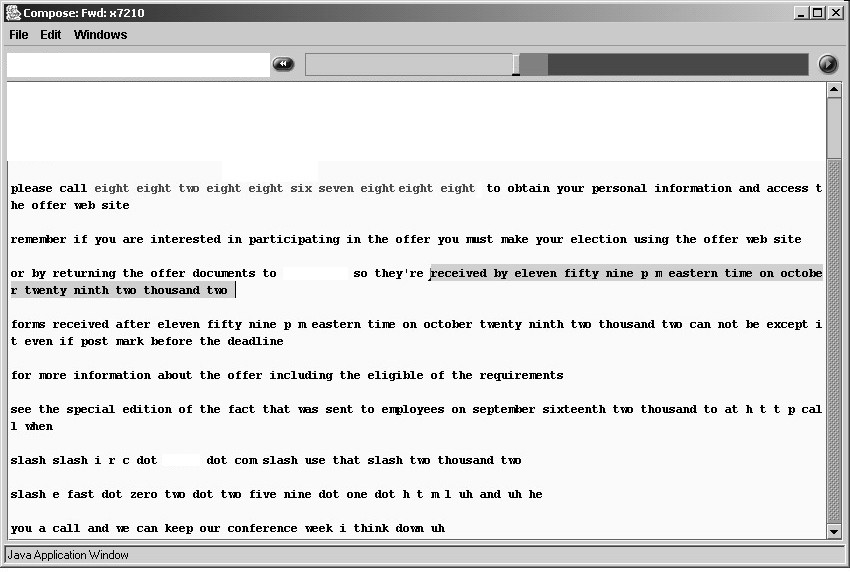
\includegraphics[width=\columnwidth]{figures/whittaker2004.png}
  %\caption{Semantic speech editor \citep{Whittaker2004}}
  %\label{fig:semanticeditor}
%\end{figure}

%, which has been shown to improve the speech and
%accuracy of audio search \citep{Ranjan2006,Whittaker2000} and comprehension
%\citep{Vemuri2004}. Word-level timing information, also allow users to edit
%speech using a text-based interface \citep{Whittaker2002,Burke2006,Rubin2013}.
%Even with imperfect transcriptions, editing using this technique is faster and
%as accurate as acoustic editing \citep{Whittaker2004}.

%Later systems have improved these interfaces with editing \citep{Burke2006},
%confidence shading \citep{Burke2006} and highlighting breaths, pauses and
%repetition \citep{Rubin2013}.

In summary, \citet{Whittaker2004} found that semantic editing of speech in
voicemail is faster and as accurate as using waveforms.  \citet{Sivaraman2016}
found that for editing discussions, semantic editing is a more accessible
alternative to waveform editing. Systems have been developed for audio and
video production \citep{Casares2002,Berthouzoz2012,Rubin2013}, but these were
mostly designed without prior user requirements, and the studies were informal
and used amateur participants. In this paper, we describe the design of our
system, which is based on the results of a published pilot study, and present
our formal study, which uses real content and professional users in an
uncontrolled working environment.

%, however most of these were
%developed without prior user requirements, none of them were tested in a formal
%user study and the informal studies that were conducted used amateur
%participants. Additionally, these In this paper we introduce Dialogger, a semantic speech editing
%system whose design is based on real-world requirements, and present the
%results of a formal user study of the system in an uncontrolled professional
%working environment.

%These studies have demonstrated the potential that transcript-based interfaces
%have for improving the navigation and editing of audio content. However, they
%have not yet been tested under real-world conditions.



%In this section, we review
%the results of the study and how it shaped the design of our system, before
%describing the features and the interface.



%We created our prototype semantic editing system `Dialogger' to assist
%specifically with the logging and rough editing stages of radio production.
%Dialogger allows users to upload audio recordings which are then transcribed
%and presented in a text-based interface that allows them to navigate and edit
%the audio using the transcript.  Dialogger then allows them to export their
%edit directly into a digital audio workstation (DAW) without loss of quality,
%where they can continue with their normal production workflow.

%In order to determine how these technologies would be best applied in the
%context of radio production, we conducted a short pilot study of radio
%production at the BBC, the results of which are more fully documented in
%\citep{Baume2015}.

%, which explored the workflow, roles, motivations and
%environmental factors.

\section{System requirements}\label{sec:requirements}
Our interest in applying semantic editing techniques to radio production first
emerged from a pilot study we conducted at the BBC \citep{Baume2015}.  In this
section, we discuss the findings of the study and the resulting system
requirements for our semantic editing system.

\subsection{Pilot study}
The objectives of the pilot study were to discover how
radio programmes are created, and to identify any opportunities to improve the
process.  Three representative programme types were studied: a
news bulletin, a drama and a documentary. The producers of each programme were
observed and interviewed to fully document their workflow, which took between
half a day (for news) and four days (for the documentary).

The main finding of the study was that many producers prefer to work with
text-based representations of audio, rather than working with the audio
directly. For example, the producers of the documentary `logged' each interview
they recorded by transcribing it themselves, or by
paying a third-party service to write a full transcription.  They then used the
transcripts to select which bits they wanted to use, and copied the text to
create a rough script of the programme. Once the script was mostly complete,
they had to find and cut each piece of audio for the programme to create what
is known as a `rough edit'.  Both the logging and rough edit processes are very
time-consuming for the producer.  From this study, we identified an opportunity
to apply semantic speech editing techniques to these parts of the production
workflow.

\subsection{Transcripts}
Radio programmes are assigned a slot in the broadcast schedule, so producers
have a strict deadline for finishing their programme. Programmes are often
scheduled about three weeks in advance, but sometimes as little as a week in
advance. This means that producers have very little time to spare. If a
programme's budget allows, interview recordings can be sent to a transcription
service where they are transcribed by a person within about 24 hours. However,
most programmes do not have the budget for this, so the producer transcribes
the recordings themselves.

Transcripts are used to help the producer make editorial decisions, but are
usually not published. For this reason, the transcripts only have to be
sufficiently accurate to use for editing. Both \citet{Whittaker2004} and
\citet{Sivaraman2016} found that the errors in the transcripts did not prevent users
from being able to edit using them. However, both also found that
users wanted to be able to fix incorrect words in the transcript.

Our semantic editing system needs to be able to produce a transcript quickly
and cheaply. It should be accurate enough to be useful for editing, and allow
for correction where necessary.

\subsection{Editing}
There are already well-established systems and software in place for producing
radio programmes. Producers use a digital audio workstation (`DAW') to select
the parts of each interview that they want to use in their programme, and to
arrange them into a narrative. The BBC provide two different DAWs -- dira!
StarTrack (made by SCISYS) and SADiE (made by Prism Sound). Some producers
prefer to use other DAWs, but as installation of software is restricted on
corporate computers, they must use their personal computers.

Waveforms are used to visually represent audio in the DAW to help the user
navigate the recordings. The edits performed in a DAW are `non-destructive'
because the original recordings remain untouched. This allows the producer the
flexibility to adjust or undo their decisions at any point during the editing
process.

Specialist sound engineers (known as `studio managers') are sometimes brought
in on the last day of production to ensure that the sound is well balanced, and
to do any advanced editing that is required. This includes removal of
unwanted `umm's or breaths in a process called `de-umming'. Being able to
de-umm speech in a way that is inaudible to the listener is a skilled task that
requires precision and experience.

Music is often included in a programme, either as a theme tune, a short
interlude or in the background. Producers select the music, often from their
personal collection. However, a number of services are also used for finding
suitable commercial or rights-free music, such as Audio
Network\footnote{\url{https://www.audionetwork.com/} (accessed 15.08.2016)}.
The music is added and edited using the DAW.

At the end of the editing process, the producer's supervisor (known as the
`editor') listens to the programme with the producer to give their feedback and
sign-off. As part of this process, they both listen out for repeated words or
phrases. However, this is only usually a problem in drama production where
multiple takes of the same lines are recorded.

Our semantic editing system needs to be able to select and arrange parts of
audio recordings. Given that there are established radio production
systems for advanced tasks such as de-umming and addition of music, it also
needs to be able to integrate with these so that it can be used in 
professional radio production.

% - Select parts of recordings and arrange into order
% - 

% Transcription
% X Need transcripts quickly
% X Not much money for transcripts
% X Transcripts aren't published, need to be good enough (Whittaker2004)
% X Whittaker says that correction would be good
%
% Integration
% X Existing system in place for broadcasting
% X Currently use waveforms
% X Must be non-descructive
%
% Web-based
% X New software can't be installed
%
% Drag and drop
% X Production involves picking bits out of interviews
% X Sorting, trying out different orders
%
% Umms/breaths
% X De-umming is skilled and done in DAW
%
% Music editing
% X Music discovery is done using existing systems
% X Editing is done in DAW
%
% Repeats
% X Repeats don't happen in interviews, only in drama really

\section{System design}
This section describes our system design, as guided by the requirements set out
in Section~\ref{sec:requirements}, followed by a description of the system.

\subsection{Transcript}
Three factors were considered when choosing a transcription method --
turnaround time, cost and accuracy. Manual transcriptions are nearly 100\%
accurate, however they are expensive (about \$1 per minute) and slow (typically
24 hours). Automatic transcriptions are imperfect, but cheap (about \$1 per
hour) and fast (x2 real-time). Our system requires quick and cheap transcripts
that are sufficiently accurate, so we chose to use automatic transcripts
generated by a state-of-the-art commercial web
service\footnote{\url{https://www.speechmatics.com/} (accessed 15.08.2016)}.

Automatic transcriptions were also used by \citet{Whittaker2004} and
\citet{Sivaraman2016}, but \citet{Berthouzoz2012} and \citet{Rubin2013} chose
to use perfect transcripts from a crowd-sourcing service. \citet{Hyperaudio2016}
used aligned subtitles and \citet{Casares2002} used a combination of subtitles
and speech-to-text.

\subsubsection{Accuracy}\label{sec:transcript}
In an informal evaluation of our speech-to-text system which used 48 hours of
mixed-genre television content, it had an overall word error rate of 47\%.
However for news content, which is clearly spoken by a native speaker, this
dropped to 16\%. As the speech on radio programmes is similar in nature to
speech on television news, the error rate was comparable. However recordings
with non-native speakers or significant background noise had a higher error
rate. For comparison, the reported error rate of the system used by
\citet{Whittaker2004} was 28\%, and for \citet{Sivaraman2016} it was 10\%.

\citet{Whittaker2004} and \citet{Sivaraman2016} found that users want to be
able to correct the transcript. We designed the system so that users can change
words by double-clicking them, typing the correct word and pressing enter.
\citet{Casares2002} also provided correction functionality, but the other
systems did not include this feature as they used perfect transcripts.

\subsubsection{Speed}
The time taken by the transcription service to process each uploaded recording
was approximately half as long as the length of the recording. The time
depends primarily on the length of the recording but also on noise, accents and
the complexity of the speech.

\subsubsection{Additional information}
The speech-to-text system we chose to produce transcripts generates
additional information from the audio. It attempts to identify the people
speaking in the recording by their gender and a number (e.g. [M2], [F5]). Also,
for each word, the system assigns a value between 0 and 1 of how confident it
is that the word is correct. We decided to include these extra pieces of
information, as they should both be useful to the producer.

We labelled each paragraph in the transcript to indicate where different people
are speaking. \citet{Rubin2013} also identified speakers by placing their
respective parts of the transcript in different columns.  However, this
approach limits the number of speakers by the number of columns that can be
displayed. By labelling paragraphs, we are able to support multiple speakers.

We used the confidence value for each word to shade words that fell below a
threshold, using a technique known as `confidence shading'. This has previously
been used by \citet{Burke2006} for navigation of speech, but it has not yet
been used for semantic editing.


%The speech-to-text system can recognise esoteric words like `ribosome' and
%`ARPANET', but can struggle with colloquialisms and casual conversation. If the
%recording is too quiet or noisy, or a word isn't in its dictionary, the system
%makes a best guess (e.g. `subbuteo' was translated as `some beauty'). It also

%Recorded interviews have at least two people speaking (sometimes more), so it
%is helpful to know where in the recording they are speaking. Our system
%attempts to detect where there is a change of speaker, then inserts a new 
%paragraph for each speaker with a unique label including their gender (e.g. M2, F5).
%We selected this layout over Rubin's approach of having separate columns
%for each speaker so as to allow more than two speakers.

\subsection{Interface}
Our semantic editing system needs to be able to select and arrange parts of
audio recordings. To achieve this, we used the same drag-and-drop interface as
\citet{Hyperaudio2016} as it is a simple method for extracting and re-ordering
clips. It also allows clips from different recordings to be added and
re-arranged. \citet{Casares2002}, \citet{Sivaraman2016} and
\citet{Berthouzoz2012} used a select/delete interface, where parts of an
individual transcript can be chosen or removed, and \citep{Whittaker2004} and
\citet{Rubin2013} used a cut/paste/delete interface.

We designed our interface to be browser-based, as the BBC corporate policy
meant that it was not possible to install new software on the producers'
computers. This came with the added benefit of allowing users to work from
anywhere in the world on any operating system, but the downside that they have
to be connected to the Internet.

\subsection{DAW integration}
Our system needs to be able to integrate with the existing radio production
tools. We designed Dialogger to be used as the first stage of the editing
process, and to smoothly integrate with the DAWs that are used in BBC Radio. We
achieved this by providing a novel features to export edited content from our
system, either as a .wav audio file or as an `edit decision list' (EDL).

The first option exported a single .wav audio file of the edit. This method is
a `destructive' edit, in that it throws away the pieces of the recording which
weren't selected. 
The other option exported an EDL, which contains metadata about which parts of
an audio or video recording make up an edit. These can be read by the
two most common audio editors used at the BBC -- SADiE and dira! StarTrack.
This method is `non-destructive' because the full original recordings are
retained and the edit points can be re-adjusted in the audio editor.  Following
early informal feedback, features were added to allow the text to be printed or
exported into a word processor.

\subsection{Excluded features}
\citet{Rubin2013} and \citet{Berthouzoz2012} included detection and removal of
`umm's or breaths as this was generated as part of the crowd-sourcing service.
We did not include this functionality as we found during the pilot study that
removal of `umm's and breaths is a highly specialised task that cannot yet be
automated to a professional standard.  Additionally, as our system is based on
speech-to-text, information about the position of `umm's and breaths is not
available.

We did not include features for adding or editing music. During the pilot study,
we found that specialist tools are already used for finding and choosing music,
and that editing of music is already efficiently handled by the DAW.
\citet{Rubin2013} included features for finding music tracks and creating loops
within them.

\citet{Rubin2013} also included detection of repeated words and phrases. We
chose not to include this, as our pilot study found that repeats are only an
issue in drama production. As the production of drama involves a very different
workflow \citep{Baume2015}, we chose not to include drama production in our
system design or study.

%\begin{figure}
%\centering
  %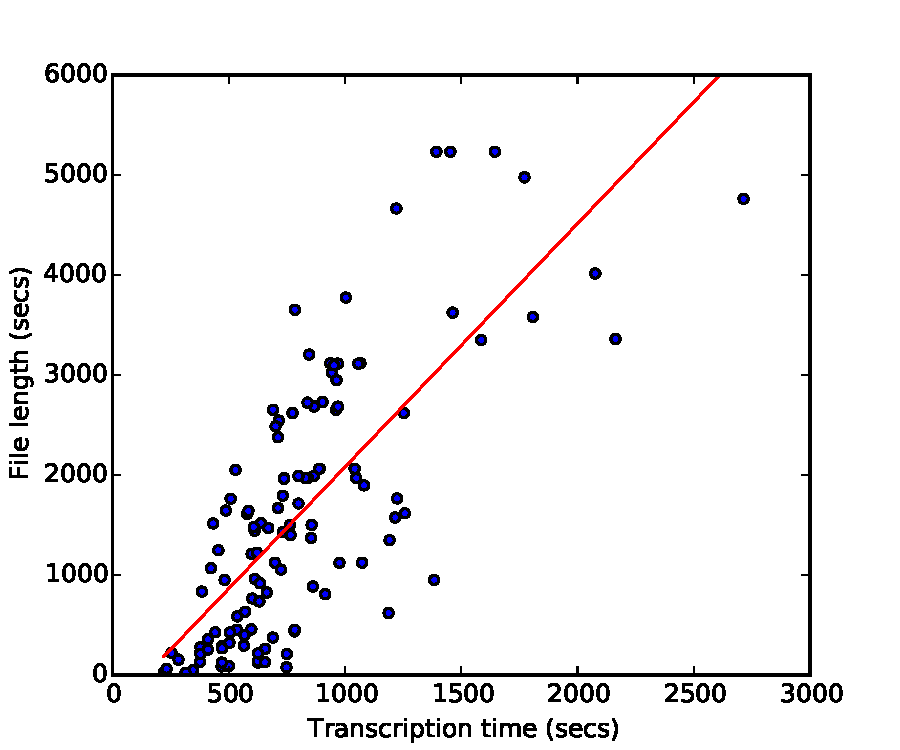
\includegraphics[width=\columnwidth]{figures/transcribetime.pdf}
  %\caption{Time taken to transcribe each recording with linear trend line}
  %\label{fig:transcribetime}
%\end{figure}

\subsection{System description}
This section gives a brief overview of Dialogger, including its functionality
and operation.  A screenshot of the interface and numbered list of the main
features are shown in Figure~\ref{fig:interface}.  A live demo of the system
is also available\footnote{\url{https://speecheditor.virt.ch.bbc.co.uk/demo}
  (accessed 15.08.2016)}.

\begin{figure*}[ht]
\centering
  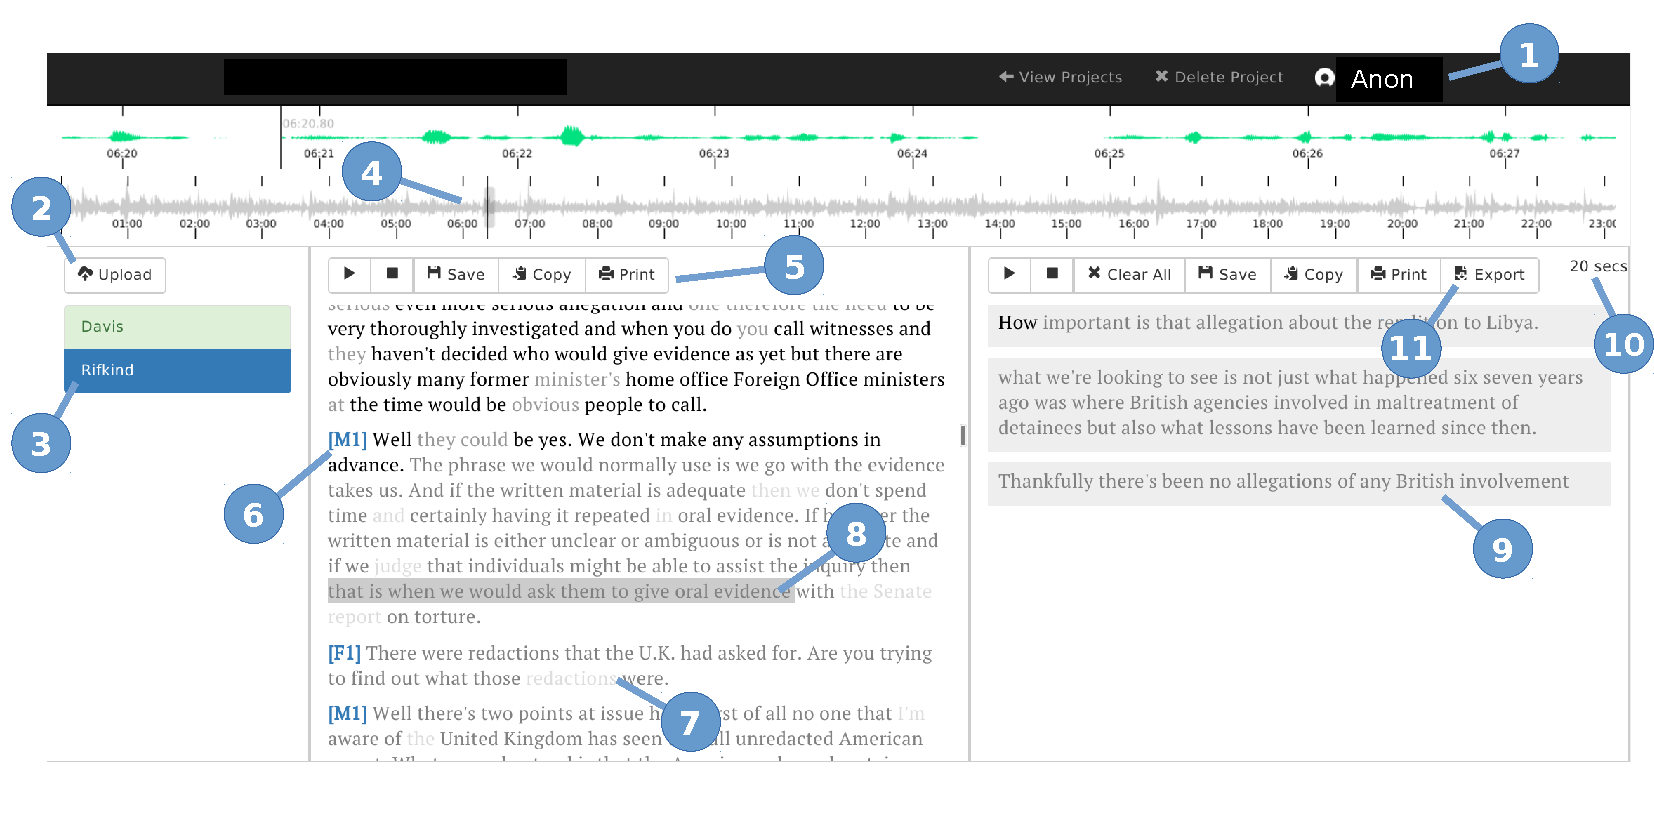
\includegraphics[width=\columnwidth]{figs/interface-labels.pdf}
  \caption{Screenshot of the user interface with highlighted features: (1)
    individual user accounts and projects, (2) upload of audio recordings, (3)
    list of uploaded recordings, (4) waveform display of currently selected
    recording, (5) toolbar with playback, save, copy and print functionality,
    (6) transcript of selected recording with speaker labelling and word
    editing, (7) confidence shading, (8) transcript selection with
    drag-and-drop editing, (9) listing and re-ordering of edits, (10) duration
    of edit, (11) export edit to audio file or digital audio workstation.}
  \label{fig:interface}
\end{figure*}

\subsubsection{Functionality}
Dialogger is web-based speech editing tool that can be accessed from anywhere
using a web browser.
Users can upload their own speech recordings into a project in their individual user
account. Each recording is automatically transcribed at around twice
real-time speed, with a word error rate of approximately 16\%.

The interface displays a list of the user's recordings on the left, the
transcript of the selected recording in the middle, and a blank workspace on the
right. The waveform of the selected recording is also shown at the top.
Users can play a recording, and navigate it using either the transcript or the waveform.

The transcript is divided into paragraphs at points where the speaker
changes. Each paragraph is labelled with the speaker's assigned identity, including
their gender (e.g. [M3]). Words that might not be correct are shaded grey, and
incorrect words can be fixed by the user. Buttons at the top of the transcript
allow the user to print the transcript, or copy it into a word processor.

Recordings can be edited by highlighting and dragging words from the
transcript to the workspace on the right, which creates a clip. Multiple clips
can be created and re-ordered to produce an edited version. The edited version
can be played to allows users to preview the result. The user can save their
edit to revisit later.

The interface displays the total duration of the edit. The edited version can
be exported as either a .wav audio file, or as an edit decision list (EDL) for
a digital audio workstation (DAW).

%TODO Add block diagram?
\subsubsection{Operation}
The operation of the system is described below as a typical user journey. Each
feature is numbered and shown in Figure~\ref{fig:interface}.

Users access Dialogger by navigating to a web page in their browser. They start
by logging into the system using their account (1) and create a project where
they can upload their speech recordings (2) that appear in a list on the left
(3). Each recording is automatically transcribed. When it is opened, the
waveform appears at the top and the transcript appears in the middle section.
The recording can be played (5) and navigated by using the waveform (4) or by
clicking on a word in the transcript (6). The transcript shows where different
people are speaking with labels at the beginning of each paragraph. Words which
are likely to be incorrect are shaded grey (7), known as `confidence shading'.
Incorrect words can be fixed by double-clicking them and typing the correct
word. The audio can be edited by selecting a range of words (8), then using
drag-and-drop to place it in the area to the right which creates a clip (9).
Clips can be re-ordered and deleted. The total duration of the edited clips is
displayed (10). The edited clips can be exported as a .wav audio file or as an
EDL (11) for further editing in a DAW.

%During this period there was no easy
%way to listen to the audio, so although they know \textit{what} was said, they
%don't know \textit{how} it was said.

%After editing using the transcript, the producer must go back to find and cut
%each piece of audio they wanted to use in the programme, known as a `rough
%edit'. Moving from audio to text and back again is costly, but is considered
%by the producers to be worthwhile. We believe that by linking audio and text
%representations together in a single editing system, it would be possible to
%work with either representation without incurring the cost of converting
%between the two.

%The pilot study also found that some of the functionality included in previous
%studies is already efficiently handled, or cannot yet be automated. For
%example, advanced music discovery platforms like Audio
%Network\footnote{\url{https://www.audionetwork.com/}} allow producers to
%quickly find music tracks of the right length, and removing `umm's or breaths
%from speech transparently is a skilled task that requires fine editing and
%human judgment.

 %It found that producers of speech radio prefer to work with
%text-based representations of audio rather than with the recordings directly.
%Their workflows are primarily paper-based which creates extra work when moving
%between paper and audio. Creating a link between the words on the paper and
%their location in the audio recordings could significantly improve the
%production workflow.

%The study also identified opportunities to apply semantic audio technology
%and interaction design to radio production tasks. Lots of time is spent
%cleaning up recordings by removing redundant speech, which could be fully or
%semi-automated. Segmenting speech content by speaker would make a positive
%impact on most speech-based tasks. Finally, drama productions could benefit
%from an easy way to compare multiple takes of the same scenes.

%\subsection{Design}
%We designed Dialoger to play to the strengths of transcript-based editing by
%focusing on the key features for logging and rough editing, and integrating
%well with the current production workflow. We excluded some features like
%removing `umm's or adding music, which are better handled by existing systems
%or techniques.  We also excluded detection and handling of repeated phrases, as 
%this technique is only used in drama production.

%This section describes the design, features and implementation of the
%prototype.




%\subsubsection{Transcription}
%\subsubsection{Layout}
%The interface is laid out so that the workflow operates from left to right.
%Recordings are uploaded and listed on the left (2), the transcript of the
%currently selected recording is shown in the middle (6), and clips are
%created and exported on the right (9). The waveform of the currently selected
%recording is shown at the top on a dual time-line (4), where the bottom
%waveform shows the entire recording and the top is a magnified display of the
%current position.

%\subsubsection{Navigation}
%Users can navigate the selected recording by clicking on a word in the
%transcript, which seeks to that position and starts playback, or by clicking on
%the waveform to jump to a specific time. Playback can also be controlled using
%buttons in the toolbar above the transcript (5).

%The text before and after the current playback position is coloured black and
%dark grey, respectively, to indicate the current playback position in the
%transcript.  Words which the speech recognition system is not confident about
%are shaded in light grey (7), known as `confidence shading'.


%\subsubsection{Editing}
%An audio clip can be created from the transcript using drag-and-drop.  The user
%selects text from the transcript (8) then drags and drops the selection in the
%space to the right.  Each clip is contained in a shaded box (9) which can be
%re-ordered by dragging them up and down, or deleted by clicking an `X' in the
%top right of the box.

%The clips can be played using the playback buttons at the top, or by clicking
%on a word. The total length of the clips is displayed above the text (10).


%\subsection{Implementation}
%The system was implemented using web standards, which allowed a consistent
%experience on any recent web browser, and avoided the need to install any
%software locally. The front-end was written in Javascript using the Hyperaudio
%\citep{Hyperaudio} and peaks.js \citep{Peaks} libraries, and the back-end was
%built using Node.js and MongoDB running on a virtualised Ubuntu server.
%Communication between the two was done through a REST API.

\section{Methods}\label{sec:methods}
We designed and conducted a formal study to explore how radio programmes are
currently created, to evaluate how Dialogger performs in professional radio
production, and to measure its impact on the production workflow. 

\subsection{Design and procedure}
Gaining access to radio producers can be difficult as there are not many of
them and they are normally very busy. A number of unrelated
studies on television production systems have previously been conducted
\citep{Engstroem2010,Perry2009}, but we were unable to find any studies at all
which used radio producers. One study attempted to recruit radio producers but
was unsuccessful because the producers were ``so highly tasked''
\citep{Kim2003}. However, we were able to recruit professional radio producers
from the BBC due to the access available to us as an internal research
department.

Radio producers find it difficult to step away from their day-to-day work for
too long. To account for this, we designed our study to take place at their
desk and to overlap as much as possible with the work they already need to do.
Our within-subjects study was primarily qualitative and was conducted through
observation and interviews. We also recorded task completion time and metrics
about the usage of each feature. The design was made up of the following five
stages:

\paragraph{Stage 1}
    A semi-structured interview to learn about the participant's
    background, their existing production workflow and the tools they used as
    part of that. The interviews typically took between 30 and 40 minutes.

\paragraph{Stage 2}
    A short training session on the semantic editor interface, followed by
    a usability test.  Each participant was trained on the interface's
    functionality using a pre-written `tool-tip tour', in which the participant
    was presented with a sequence of instructional pop-up dialog boxes overlaid
    on the interface.  This ensured consistency of training between
    participants.

    The usability test involved giving the participant a series of verbal
    instructions for common tasks that utilised all of the functionality of the
    interface. The investigator observed their actions, but gave no other
    directions unless requested. They noted any unexpected behaviour, stumbling
    blocks or other failures.

\paragraph{Stage 3}
    Observing the participant as they produce a radio programme.
    Each programme is composed of a number of interviews on the same topic. 
    We observed the participant while they logged and rough-edited two
    different interviews for the same programme. They did this for one
    interview using their existing production workflow, and the other using
    Dialogger.
    
    The order of the conditions was counterbalanced to
    eliminate bias and the actions of the participant on Dialogger were logged
    electronically. After the observation, they were asked to rate each
    condition using the NASA Task Load Index metrics
    \citep{Hart1988}.

    The tasks were performed as part of the production of a real radio programme,
    and the observation was done in the participant's normal work environment.
    The investigator sat beside the participant during the task and made notes
    on the workflow, tools, generated metadata, usability issues, task
    completion time, and unexpected reactions or usage.

\paragraph{Stage 4}
    A semi-structured interview about the participant's experience of each
    system and how they compare. The primary objective of this interview was to
    extract the advantages and disadvantages of each workflow. The interviews
    typically took between 30 and 60 minutes. The audio from each interview was
    recorded and transcribed to allow a full analysis.
    %The questions asked were:

    %\begin{itemize}
        %\setlength\itemsep{0em}
      %\item Which aspects of the existing system did you / did you not find useful?
      %\item Which aspects of the prototype system did you / did you not find useful?
      %\item Overall, which system did you prefer and why?
      %%\item Did the prototype change the way you made the programme? If so, how?
    %\end{itemize}

\paragraph{Stage 5}
    Each participant was then given access to Dialogger 
    for a further month, and was invited to continue to use it should they
    wish. Each week, they were asked via email whether they had been using the
    system, and if so, which features they valued most/least or were missing.
    During this time, their usage of Dialogger was also logged electronically.

\subsection{Participants}
We invited professional radio producers with at least five years of experience
by sending an email to departments in BBC Radio that create pre-produced
factual programmes.  Drama programmes were excluded from the study as their
production workflow involves making multiple recordings of lines in a script
and selecting the best ones \citep{Baume2015}. This is a sufficiently different
process to other programme genres that it warrants a different interface.

Five participants (P1--P5) were recruited (4 male, 1 female) who each had
between 6 and 20 years experience in working as a radio producer. Although we
had a small number of participants, the experience of the
producers and the depth of the study means that their feedback should carry
significant weight. Five participants is also considered sufficient for
identifying most usability problems \citep{Nielsen1993}.

During the experiment, the participants worked on programmes of different
lengths from a range of genres:
P1 produced a single 27-min documentary, %plus 50-min for WS
P2 produced a 27-min documentary as part of a ten-part series,
P3 produced a single 45-min documentary,
P4 produced a 14-min archive programme
(based around material from the archive) as part of a ten-part series, and
P5 produced a single 27-min magazine show (covering multiple stories on a
single theme).

\subsection{Analysis}
The notes from the pre-interview, usability test and observation were analysed
to look for common issues, unexpected reactions and unanticipated usage. The
post-interviews were transcribed, and coded using the software package RQDA
\citep{RQDA}, to identify common themes. The electronic usage logs from the
semantic editor interface were analysed to calculate and graph usage patterns.

\section{Study results: Existing workflow}\label{sec:resultsexisting}

%\subsection{Observation}
%During the first interview, participants worked with the investigator to
%identify a particular task in their workflow that would form the basis of the
%observation. In every case, logging and rough editing of an interview was
%selected, as this process takes a long time, is considered tedious and would
%benefit from automatic transcription.

%Due to the pressured and changing work environment, the observation had to fit
%around the editing requirements at the time of observation. This meant that P4
%and P5 did not do any logging during observation.

This section describes the existing radio production workflow. The process is
documented as described by participants (P1--P5) in the interviews (Stages 1
and 4) and as witnessed by the investigator during the observation (Stage 3).

\subsection{Pre-production and recording}
When a programme is commissioned, the producer starts by researching the
subject in detail to identify a compelling story and to find the best
contributors. This is done by reading, listening and watching existing material
on the subject, and finding and talking to relevant people. During this time
they also recruit a presenter.

The producer organises the programme by writing a `script'. This is
primarily used to help them structure their thoughts, but also to help
communicate with the presenter over email.
%The scripts contain varying amounts
%of detail, depending on the subject and the individual producer. Some will
%eventually include a full transcription of the programme, whilst others will
%remain as a bullet-point outline.  The scripts are written using Word, with P2
%also using `MindManager' mind mapping software.
%The script can be created at any point during production, but is often started
%during the research stage.
In the study, P1, P2 and P5 started their scripts
during the research stage by writing an ordered list of bullet points of topics
%to cover and a list of draft questions to ask contributors.
and questions.
P3 and P4 waited
until after they had done some interviews to start the script, as they wanted
to structure the programme around the discussions that they recorded.

%P3 and P5 updated the script after every edit to ensure they were always in
%sync. This added significant overhead but gave them a visual structure to
%follow when making the final changes.

After researching the topic, the producers then arranged interviews with
contributors and recorded them with the presenter either in a studio, an external
venue or via a telecommunication link.

\subsection{Logging}
Once material has been recorded, the next step is for the producer to select
which parts of the audio they want to use in the programme.
Interviews recorded for speech radio often cover complex topics in fine
detail. Keeping track of all the points raised and forming a compelling
narrative from them is a challenge.

\textit{``All the interviews overlap with each other terribly, and have got
  similar themes.''} (P4)

The skill of the producer is to \textit{``separate the wheat from the chaff''}
(P1, P3, P4) and to find the clips which will make an interesting programme.

\textit{``That's the basis of my job - to find great stuff and put it together.
  It's not difficult putting it together, it's finding the great stuff and
  finding connections between it. Getting rid of the non-great stuff is
  challenging and time-consuming, and it requires mental processing.''} (P1)

This selection process is aided by creating `logs' of the interviews.  Logging
helps this process by allowing producers to see, on screen or on paper, what
was said in each interview, when and by whom, without having to listen to it.
This allows them to quickly find and share the pieces that they want to use in
the final programme.  It also helps them structure their thoughts, identify
themes running through discussions, and make links between different
interviews. However, the sheer quantity of recordings means this process adds
significant overhead.

\textit{``you've got an average of 45 mins per interview and in a series of
  three programmes you've got seven per programme, that's a lot of work''} (P3)

\begin{figure}[ht]
\centering
  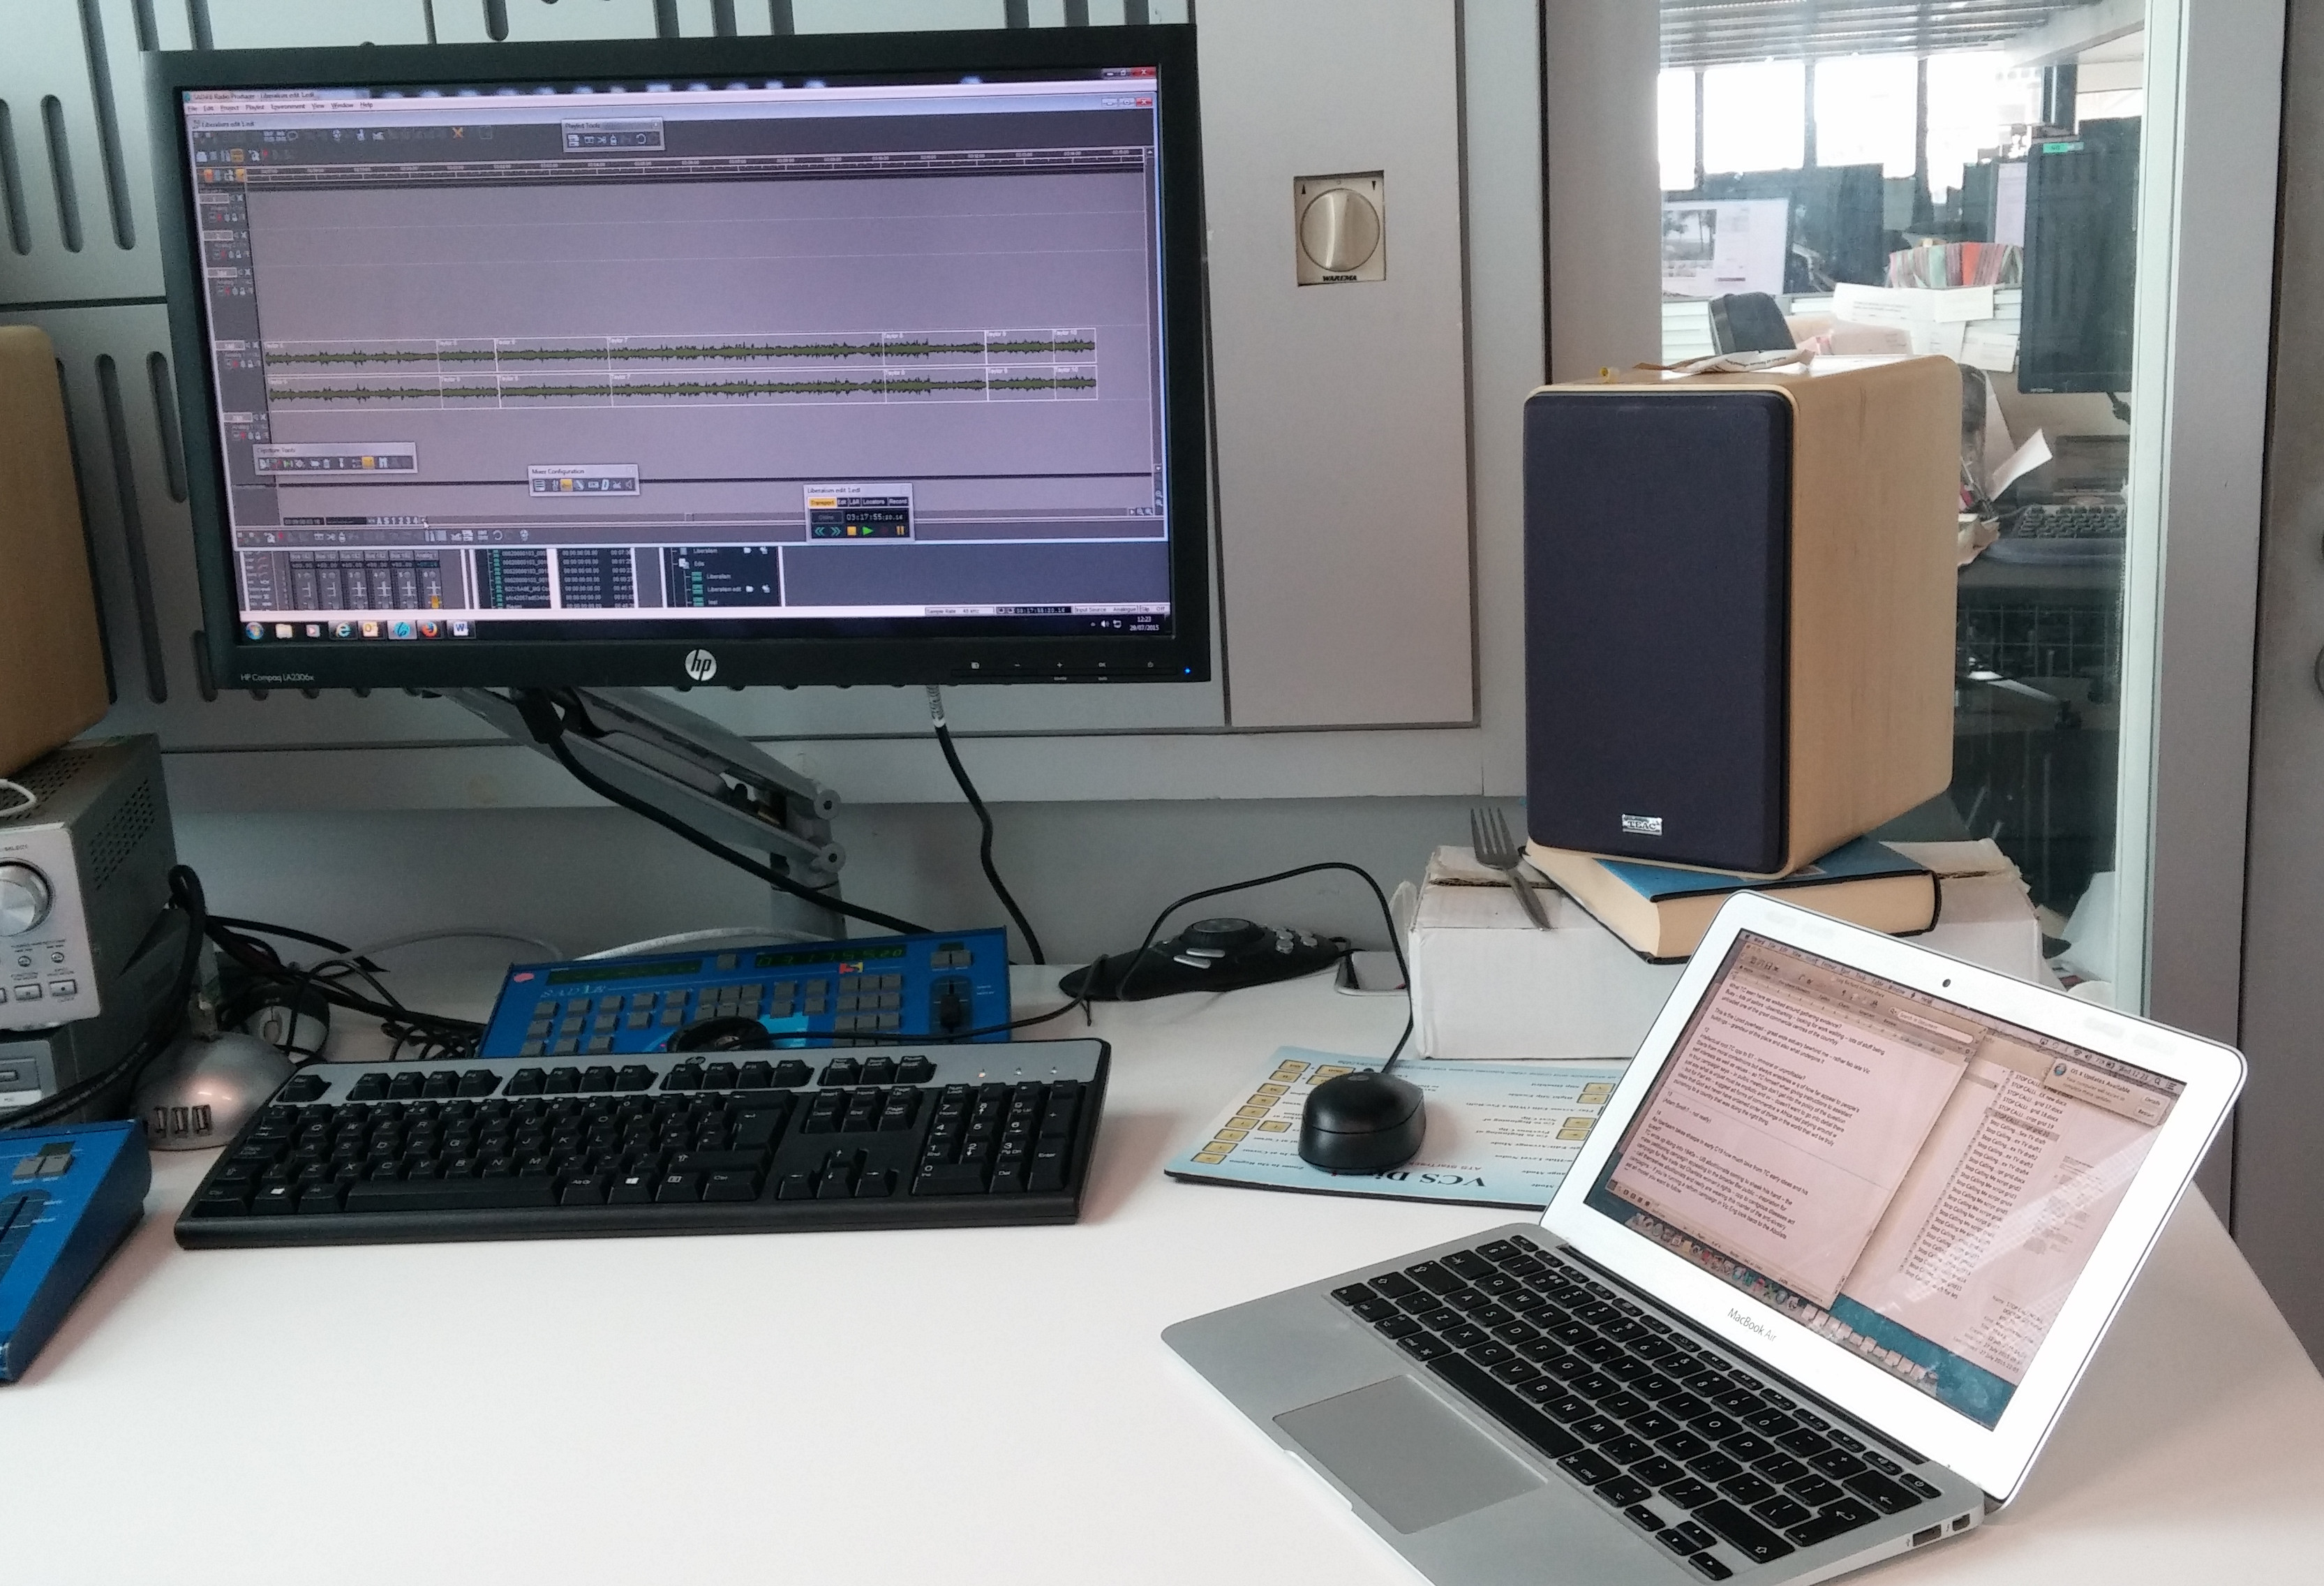
\includegraphics[width=\columnwidth]{figs/phil-desk.jpg}
  \caption{P3 logging interviews with a digital audio workstation on the desktop
    PC and word processor on the laptop}
  \label{fig:desk}
\end{figure}

Logs are usually written by the producer themselves. As they have done the
research and are normally present at the recordings, they can use their memory
to navigate the material and use their experience to quickly determine which
parts are relevant. Some programmes that are under particular time pressure
will use a third-party to create a verbatim transcript of a few interviews
\citep{Baume2015}, but most do not because it is too expensive.

Writing the logs takes a lot of concentration as the producer must listen to
what is being said, work out how it ties in with other contributions and the
story, and make swift judgements on whether it should be used.

\textit{``one of the slightly exhausting things about doing it is the level of
  concentration you have to maintain to make good decisions, remember where
  everything is, what you've got, is kind of strained rather by having to just
  do shleppy tasks like moving the sound and logging interviews''} (P3)

Additionally, many producers find that the open plan office in which they work
is not the best environment for writing logs. For this reason, many choose to
do it away from the office. 

\textit{``I typically do this at home because I find it a much less distracting
  environment. It does require quite intensive concentration so you don't miss
  something.''} (P1)

The high level of concentration required, combined with the repetition of 
typing and listening to the interview again means that producers need to take
regular breaks.

\textit{``it's boring and it's not very easy to be efficient at it [...] when
  I'm normally doing it I'm checking my emails, making a cup of tea.''} (P3)

In the observation, P1 and P3 wrote their logs in Microsoft Word whilst using a
digital audio workstation (DAW) to play the recording (see
Figure~\ref{fig:desk}). P5 reported that they usually followed a similar
process, but did not do any logging during observation.

P4 also did not do any logging during observation, but explained that they
would normally write their logs by hand in a notebook whilst listening on a
portable music player somewhere away from the desk, such as in a caf\'e.

P2 used a different approach. They played the recording in a DAW and used a
keyboard shortcut to create timed markers at any points of interest. By seeing
where the markers clustered, they identified where to make clips, then gave
each of the clips labels. This approach allowed them to focus more on the
audio, but didn't allow them to make any detailed notes.

The exact format of the logs varied between individuals, but they usually
contained a rough transcript of the interview with occasional timestamps and
notes. They reported that this helped them to find important bits in the
recording later on. Each producer has their own syntax, but there are
commonalities.

Timestamps were written on the logs, approximately \textit{``every 30 to 120
  seconds''} (P1) with minutes and seconds in parenthesis: \texttt{(4'20)},
for example.  This allows the producer to navigate to a particular piece of
audio much faster than they would otherwise by narrowing down their search
range.

P1, P3 and P5 would make comments for themselves in the log to help them when
editing. For example, ``\textit{[good to here, dull after]}'' or
``\textit{[trails off 9'30]}''. P1 also used a star rating system to rate the
quality of each point, for example ``\textit{[**** should use this stuff, but
  dramatically cut down]}''.

\textit{``What I sometimes do when I edit are star good bits, and I think
  that's quite a common trait.''} (P3)

Bold highlighting was also used by P1 and P3 to mark bits of the transcript
which are important and worth keeping.

\textit{``what I did was just put in bold the paragraphs I thought were worth
  [keeping]''} (P1)

Every participant that was observed logging played the audio faster than real
time at least once. This allowed them to fast-forward through parts of the
interview that may not be of interest (e.g. discussion in the background)
whilst still being able to listen out for anything they might want to use.

\subsection{Rough editing}
This stage involves extracting audio clips from the recordings which will form
the basis of a draft edit of the programme. If the recording was short and had
been recorded recently, as was the case for P4 and P5, it can be edited without
a log. In this situation, we observed that the producers listened through the
recording using a DAW and pressed a keyboard shortcut to split the recording,
usually at the beginning/end of questions/answers. They then went back and
removed unwanted segments.

If the recording has been logged, the producer will use the log to decide which
parts to select or remove. They use the timestamps written in the log to narrow
down their search area for each clip they extract. However, even with a reduced
search area, the producers find it time-consuming to find the exact start and
end point of each clip using the DAW interface.

In the study, three of the participants (P3, P4 and P5) used SADiE as their
DAW, which is provided to the producers by the BBC. However, the other two
participants chose to use other software packages that aren't formally
supported. P1 used Adobe Audition because they were familiar with the interface
and it was installed on their laptop, unlike SADiE which was only available to
them on a desktop computer.

P2 comes from a television production background and used Apple's Final Cut
Pro, which is primarily a video editor but also includes audio editing
functionality.  Similarly to P1, P2 used Final Cut Pro because they were
familiar with the interface and had it on their laptop. In addition, they
enjoyed being able to import audio directly from video content without having
to use another program to extract the audio first, and being able to use the
video `titles' feature to make written notes.

At the end of this stage, the producer will have clips of their recordings
assembled into a basic structure of their programme in the DAW. This will
normally be about twice as long as the final programme, sometimes significantly
longer (e.g. P5 created 22-hour-long rough edit for a 37-min programme). The
producers then continue to trim the edit down to a manageable length.

\subsection{Fine editing}
The next stage is to add narrative elements, known as `links' to join the clips
together into a storyline. The producer and presenter will write the links
together, using the programme script to collaborate. The presenter records
the links in a studio and the producer then assembles them into the edit.

Once all of the content has been added to the edit, the final stage is to `get
it down to time', adjust the audio volume, and to add any music or
sound effects. The speech is cleaned up by removing redundant noises (e.g.
`umm', `err', `you know') in a process known as `de-umming'. We observed that
many producers brought in an experienced sound engineer to help with any
final complicated editing.  Once the editing is complete, a final version is
rendered to a stereo audio file and added to the radio playout system for
the producer's editor to sign-off.

\section{Study results: New workflow}\label{sec:resultsnew}
This section discusses the results and themes that emerged from the evaluation
of the semantic editing interface. We start by outlining the results of the
usability test (Stage 2) before going into detail on each of the themes that
came out of the observation (Stage 3) and the final interview (Stage 4).
The coding software RQDA was used to identify the themes and to extract
suitable quotes.

%To evaluate the semantic editing interface, participants were observed while
%they used the system to log and rough edit recordings for a programme.
%Although it was designed as an all-in-one solution for putting together a rough
%edit for a programme, participants used the interface in different ways to
%integrate with their existing workflow.

%P3, P4 and P5 used the interface much as designed by using the transcript
%window to read and identify suitable clips, then dragging them across to the
%edit window and exporting the audio.

\subsection{Usability test}
Participants were first introduced to the semantic editing interface through a
usability test (Stage 2). P1 completed the test quickly and without issue,
expressing that it was easy and intuitive. The other four participants
successfully completed the test, but identified a number of minor usability
problems regarding keyboard shortcuts.

Two of the five participants (P2 and P3) kept pressing the space bar to start
and pause audio playback. This may be habitual, as it is a universal keyboard
shortcut in all DAWs. However, this feature was not considered when designing
Dialogger.  Additionally, P2 tried to use word processing shortcuts in the
interface, such as Ctrl+C and Ctrl+V to copy/paste and backspace to delete.

P1, P2 and P4 reached for Ctrl+F to search for a word they were
looking for. Although this feature wasn't explicitly implemented or mentioned in the
training, the functionality was included in the browser. The participants
remarked that it was a powerful tool for navigating the recording.

In conclusion, we found that keyboard shortcuts are more important than we had
considered when designing Dialogger.

%The interface was designed to allow users to copy the text of the entire
%transcript by pressing a `copy' button. Four of the five participants
%intuitively selected the text before pressing the copy button.  P2 expressed a
%preference to use Ctrl+C and Ctrl+V shortcuts to copy and paste text, rather
%than a drag-and-drop gesture.  Additionally, P2 said they wanted to be able to
%remove selected text by pressing backspace, or to export only selected text.
%Future versions should
%consider allowing users to apply actions only to selected text.

%Three of the five participants (P2, P3 and P5) couldn't remember the action to
%correct a word (double-click). Two of them (P2 and P3) right-clicked the text
%and looked for an option in the context menu.

%P2 confused about double waveform

%\section{New workflow}
%Following the usability study, participants were observed using the prototype
%interface to complete a common production task and interviewed about it
%afterwards. This section documents the findings.

\subsection{Navigation and editing}
Participants reported that having the transcript available in the semantic
editing interface allowed them to read and search the recordings much faster
than they normally would with a waveform.

\textit{``with having a transcript you're able to immediately scan through it
  10/15 times faster. Maybe that's an exaggeration but it feels ten times
  faster''} (P1)

The transcripts also allowed the participants to quickly cross reference what
was said in various interviews without having to listen through multiple times.

\textit{``where I'm picking shorter clips, making a point and moving on or I'm
  developing an argument between different people and cutting between them, it
  feels a lot more easy to construct that `on paper' than what I'm currently
  doing''} (P2)

%\textit{``If it's a shorter thing I'll bang it straight into SADiE and start
  %editing down to find the wheat from the chaff''} (P4)

Being able to click on a word to navigate to that point in the audio also
enabled the participants to use visual search to quickly find and listen to
bits they were looking for.

\textit{``you can do that with your eyes even quicker - zone straight in on the
  bits and that click to go  `that bit', `that sentence there', `that word
  there' ''} (P4)

Participants reported that editing with a transcript was primarily useful when
working at the sentence level. When the granularity of editing involves
removing individual words, `umm's or breaths, they said that the DAW software
is much better suited to these tasks. This supports our design decision to
integrate with DAWs.

\textit{``the real editing work actually happens after this has passed its main
  point of usefulness''} (P3)

%\textit{``I was using some interviews, some contributors recorded on one
  %ocassion, but across several programmes, several episodes in a series, or for
  %several different stories.''} (P4)

%\subsubsection{Navigation speed}

%\textit{``it took me 15 mins to read 35 mins and not just read, but read and mark
  %up''} (P2)

%\subsubsection{Time since interview}

%\textit{``you're kind of doing a paper edit on the basis of having recently
  %heard the audio''} (P3)

%\textit{``a lot of that guesswork was coming from the memory of being there at
  %the recording... realising which bits were the questions from the
  %presenter and which bits were answers.''} (P2)

%\textit{``I know I've got a doc coming up in six months time, so I'll ask them
  %some questions for that. Now then in six months time I can't remember what
  %the answer was''} (P4)

%The primary benefit of reading over listening is that you can quickly scan
%ahead and jump around with your eyes, whereas listening can only be done at a
%fixed pace. 



\subsection{Transcript accuracy}
When using the semantic editing interface, editing decisions are based
on an automated transcript which is only partially accurate. However,
participants suggested that the transcripts were, generally speaking,
sufficiently accurate for their purposes.  \citet{Whittaker2004} found that
imperfect transcripts were sufficiently accurate for voicemail editing. These
results show that this finding could also apply to radio production.

\textit{``It's clearly not 100\% in word recognition but I'm feeling it's
  certainly good enough for my rough cut purposes at this point''} (P2)

If the recording being edited was made recently, the producer can use their
memory of what was said to make sense of the inaccuracies in the
transcript.

\textit{``Both these interviews [being edited] are relatively recent so I have
  it reasonably in my mind what they've been saying. I was able to read roughly
  what there was - `okay that's that question', `I know what was in that
  question' ''} (P1)

Although most of the producers we observed only used the transcript to navigate
and edit the audio, some were interested in correcting the transcript so it
could later be shared or published.

\textit{``I'm probably posting transcripts for the whole interview. So I do
  need to go through and correct''} (P4)

Clearly, the more accurate the words in the transcript are, the less work has
to be done to correct it.

\textit{``The closer it can be to the point where you don't have to clean it up
  the better obviously, and that's quite significant honestly, that's my only
  qualm''} (P3)

%Sometimes a word is commonly mistranslated throughout the transcript, so
%providing an easy way to fix that would be a useful addition.

%\textit{``Something that would be even better is Ctrl+H  replace function''}
%(P3)


%\subsection{Speaker diarization}
%One disadvantage of working with transcripts is that you can't hear which
%person is speaking when.

%\textit{``if you can't see who's speaking - that's a disadvantage''} (P3)

%Speaker diarization technology \citep{AngueraMiro2012} can be used to try and
%identify where different people are talking. The prototype included a
%rudimentary system that attempted to distinguish speakers and guess their
%gender, however it tended to significantly overestimate the number of speakers
%which caused some difficulty. 

%\textit{``It was distracting if anything, partly because I was trying to guess
  %who was which at certain points''} (P2)

%However, in many situations the participant could tell who was who from what
%they were saying.

%\textit{``It's reasonably clear to me who's asking the questions, but actually
  %[speaker diarization] is helpful''} (P1)

%During the study it was discovered that many producers record in stereo and use
%the waveform to see where people are speaking.

%\textit{``I always pan the presenter on one side and the contributor on the
  %other so I can see where the questions are''} (P5)

%This workaround could be exploited to improve the performance of a more
%advanced speaker diarization system.

\subsection{Annotation}
%Before creating any clips, P1 immediately copied the transcript text into Word
%in order to allow them to make annotations.

%The WAVs were then imported into the DAW
%by dragging and dropping them from the file system.

%In the observation stage, it was identified that annotation is an important
%part of the production process that was missing from the prototype.
P1 and P3 copied the transcript text from the interface into MS Word. They
reported that they did this because there was no annotation functionality
available within Dialogger.

They inserted paragraph breaks, added notes after each paragraph, and
highlighted desired parts of the transcript in bold. Once the transcript was
annotated in MS Word, they went back to Dialogger, found the parts of the
transcript they wanted by scrolling though the text, then dragged and
exported each clip individually as a .wav file.

\textit{``it would be better to take raw lumps of transcripts and plonking them
  in Word because Word has higher functionality than this''} (P3)

Producers are very familiar with the MS Word interface so a later version of our
system could seek to provide a similar interface. This would allow producers to
make annotations in the same way they do already.

\textit{``With text editing, the reflexes are very much Microsoft Word''} (P4)

The most basic feature that could be added is highlighting, which is often used
to note parts of interest

\textit{``If you just put a little star or underline or something simple to
  mark things, that would be a big gain for a small change''} (P3)

%\textit{``sufficient to find the bits of the audio you want to use and to make
  %sense to the presenter.''} (P3)

%\subsubsection{Star rating}

%\textit{`` I just gave myself a detailed breakdown of what was said in the
  %interview with timecodes at questions or major new points and a slightly
  %arbitrary scoring system to say 'that's really good stuff and must get in'.
  %''} (P1)

\begin{figure}[t]
\centering
  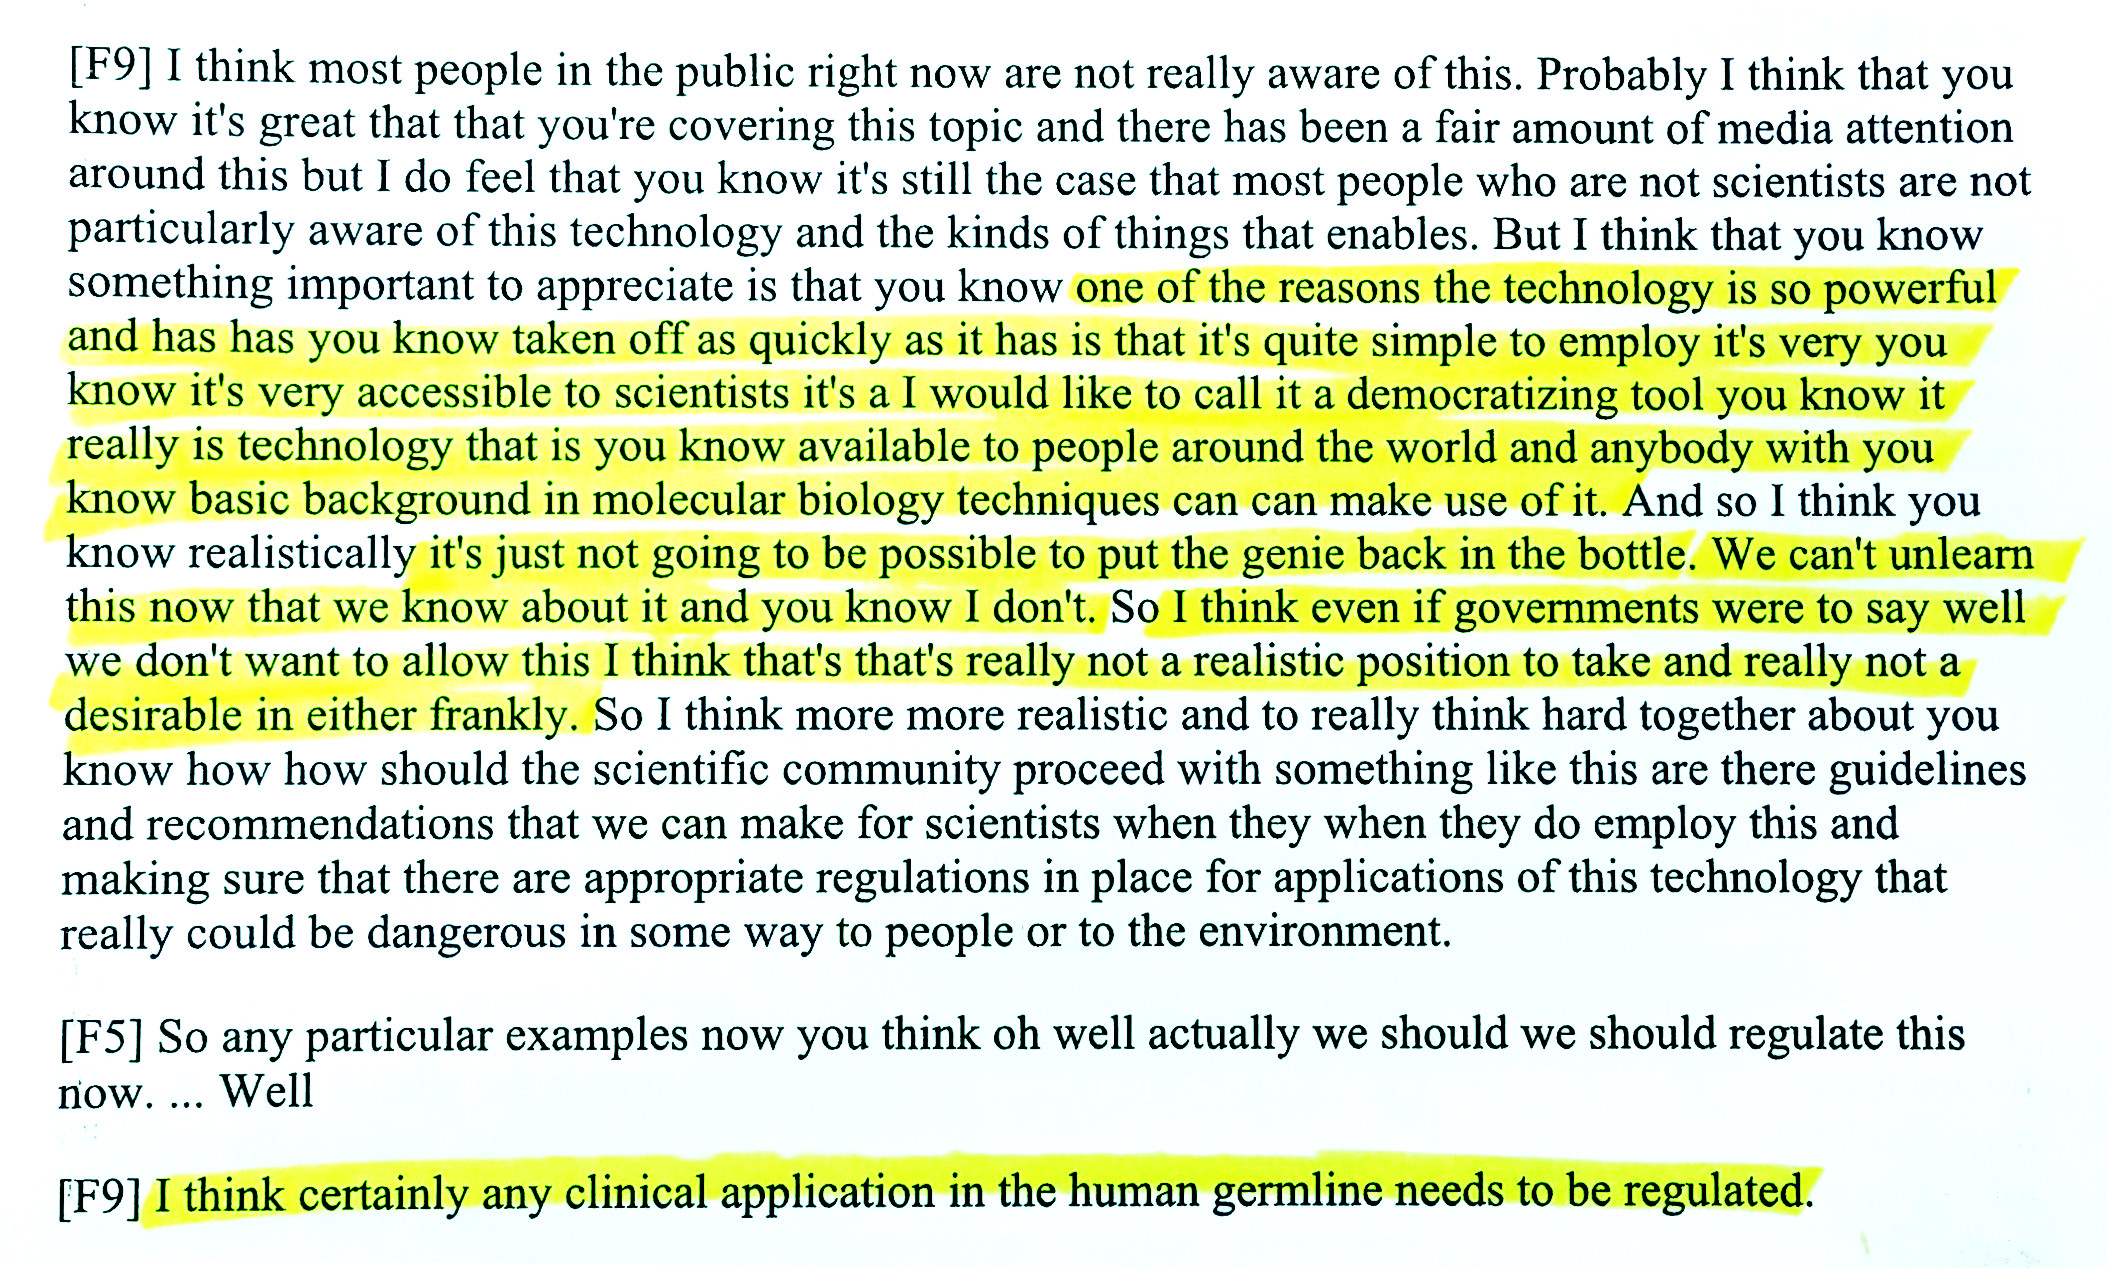
\includegraphics[width=\columnwidth]{figs/highlighting-cropped.jpg}
  \caption{P2 using a highlighter pen with a printout}
  \label{fig:highlight}
\end{figure}

\subsection{Paper}
In the observed task, after uploading their recording, P2 immediately printed
the transcript and read through it on paper so that they could work away from
the screen.

\textit{``I'd prefer to do it on page than on screen. Just easier on my
  eyes.''} (P2)

Producers reported that working on paper allowed to be productive outside of
the office, such as during their commute.

\textit{``What would be really useful would be to [...] take it away (say when
  I'm on the train going home) and I would paper edit the bits that I need''}
(P5)

%\textit{``In the office there's so much pressure and you're always doing stuff. When you
 %can step away from that, have a long commute, I can think''} (P5)

Additionally, working on paper allows them to work anywhere as it does not
require electricity.

\textit{``It's highly portable. It doesn't require any power.''} (P2)

P2 used a highlighter pen to select the desired parts of the recordings (see
Figure~\ref{fig:highlight}).  After highlighting all the pieces they wanted,
they then used the Ctrl+F text search to find the highlighted words in the
semantic editing interface.  The search feature was not explicitly included in
the editing interface, but was included in the web browser so was discovered by
some participants.

\textit{``it allowed me to get to clips very quickly from a reference point on
  a printed transcript''} (P2)

However P2 noted that having timestamps on the printout would be a faster
way of achieving the same thing.
Once they had found and clipped all of the highlighted parts in the semantic
editing interface, they exported the clips into SADiE.

Another participant explained that for an upcoming programme, they were
planning to print out transcripts from the semantic editing interface to help
them collaborate with their presenter.

\textit{``we're just going to go through it with a pencil and paper, with a
  printout, and highlight the bits we want and cross out the bits we don't.''}
(P4)

\subsection{Listening}
Part of the appeal of having a transcript is that it frees the user from
listening to the audio in real-time. It also allows users to work on paper,
away from any electronic devices. However, disconnecting the audio from the
text fundamentally changes the production process.

\textit{``Radio is made with your ears. You'll never get away from that fact
  that you need to listen''} (P4, also P2, P3, P5)

The criteria for deciding whether a piece of audio is good enough to use in a
programme is not just about what was said, but how it was said. Making
decisions on whether to keep/lose something without listening to it isn't
desirable.

\textit{``How people say things is very important and I wouldn't want to lose
  that totally.''} (P5)

There was also concern that parts which sounded great but didn't come across
as well in the transcript may have been overlooked.

\textit{``I was anxious it might not have sounded as good as it read, or that I
  might be missing bits that sounded great ''} (P2)

In the old workflow, participants occasionally played the audio faster than
real time, but that feature was not included in Dialogger.
Several of the participants noted that they would like to have this
feature added.

\textit{``it's a little bit annoying that there's no facility for that.''}
(P2)

Although faster than real time playback normally reduces intelligibility, this
would be less of a problem if the transcript was available \citep{Ranjan2006}.
This would open the possibility for playback speeds faster than are currently
possible, allowing producers to listen to content much more quickly.

\textit{``you do still need to listen through, even though you've got the text.
Therefore, it would be optimised if we could listen through quickly''}
(P4)

As listening is an important part of the production process, text should remain
linked to the audio wherever possible to allow multi-modal interaction. Once
the link is broken, re-linking the two together can be costly.

%\subsection{Interface design}
%The semantic editing interface was designed so that the user could drag and
%drop selected clips into an edit window. Although this works well for picking
%out short clips, user encountered issues when trying to select and use long
%clips as the edit window quickly filled up.

%\textit{``I found the interface quite clunky for pulling out big chunks of
  %audio.''} (P5)

%Users worked around the problem by dropping new clips between old ones, then
%re-ordering the new clip to the bottom of the list. One suggested fix was to
%have a button to append a clip of the selected text to the edit without having
%to drag and drop.

%\textit{``once you've selected on the left hand side [...] it would go to the
  %bottom of the queue, that would be a useful way of moving stuff from left to
  %right for pulling highlight clips''} (P2)

%Selecting very large amounts of text with a dragging motion also proved tricky,
%so it was suggested that clicking whilst holding shift (like in word
%processing) could fix this.

%\textit{``Just being able to hold shift and use the cursor. Selecting the text
  %was a little bit index finger intensive.''} (P4)

%Although the semantic editor is set up to select good bits, a lot of the
%participants also wanted to get rid of bad bits.

%\textit{``What you need to do is [...] to get rid of the gubbins of me talking
  %to presenters and mistranslating''} (P3)

%Some were also interested in having cut functionality that would remove the
%selected clip from the original recording. This would ensure that it can't be
%used twice.

%\textit{``You could even go further in the spirit of what it is which would
  %being able to cut and paste, delete''} (P4)

%Not all of the participants agreed though.
%\textit{``it wouldn't be something I'd be aching to be introduced''} (P1)

%\subsubsection{Stage of usefulness}

%\textit{``The transcript is useful at a later stage in the production process
  %when I've cut my programmes, when I want to export clips to the news. When I
  %need to compile a final script for a presenter''} (P2)


%\subsubsection{Quantity}

%\textit{``We've got about six hours of audio for a one hour programme, and it's
  %all just one-on-one interviews''} (P4)

%\textit{``you've got to find the right bit which is burdonsome and annoying
  %when you've got 20 interviews to do''} (P1)

%\subsection{Export}

%Stuff on export and integration

%No gaps in WAV

%\subsection{Export}
%Each participant differed in how they exported the
%content.

%P5 made a list of all the clips they wanted for the programme before exporting
%them into SADiE.  P4 made clips for three different programmes from a set
%of eight recordings. They did this by making a list of clips for one programme
%then exported them into SADiE before moving onto the next programme.

%P3 took a different approach by exporting each clip individually as a .wav file
%which they renamed.  Additionally, P3 copied the text from each clip into the
%script for their programme. They then inserted paragraph breaks between
%questions and answers, and highlighted the questions in bold so that they could
%easily identify them.

%P4 queried whether it would be possible to identify which parts of the
%recordings had already been used, so that they wouldn't be re-used in other
%programmes.

%\subsection{TV}

%Two participants suggested that text-based editing would be equally, if not
%more, useful for TV production. P2, who formerly worked in television, said
%that their workflow already followed a similar pattern. 

%\textit{``If I was making a TV show this is what I would do. I'd effectively
  %print [a transcript], read, highlight, pull a collated collection of those
  %clips or number then, then write a draft script that combined everyone's
  %interview highlight clips that I thought were relevent for telling the
  %story.''} (P2)

%The costs involved in producting TV content are much higher than radio, so
%there is a greater financial incentive in streamlining the process.

%\textit{``There's an advantage to paper edit in TV because the assemblage
  %process takes longer and you might decide you don't need particular bits of
  %archive you thought you did and [save on] transfer costs.''} (P3)

% ran out of space

\subsection{Follow-up}\label{sec:followup}
After the interviews and observations were complete, the participants were given
access to Dialogger for a further month (Stage 5). During this time their
actions were logged electronically and they were emailed each week to ask which
features they found useful, or were missing. P3 was unavailable immediately
after the study, so could not take part in the follow-up stage.

Most of the comments received in the follow-up stage were already picked up by
the first part of the study. In the remaining comments, all of the participants
said they enjoyed being able to use the semantic editor outside of the office
and at home. Some reported that they had issues uploading content with their
slow network connections, and P2 suggested that allowing multiple simultaneous
uploads would allow them to leave it running overnight.


\section{Study results: Metrics}\label{sec:resultsmetrics}
\subsection{Time}

\begin{figure}
\centering
  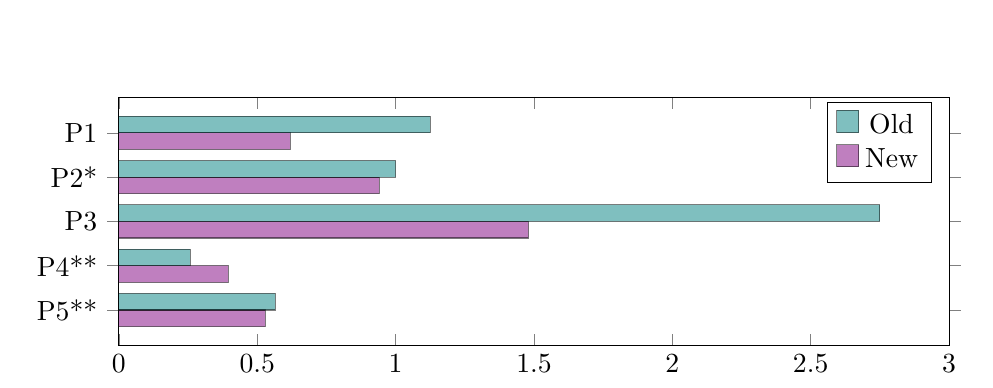
\begin{tikzpicture}
  \begin{axis}[
      width=\columnwidth,
      xbar=0pt,
      bar width=6pt,
      xlabel=Task duration / Audio duration,
      y=16pt,
      xmin=0,
      xmax=3,
      enlarge y limits=0.2,
      symbolic y coords={P1,P2*,P3,P4**,P5**},
      ytick = data,
      y dir=reverse,
      reverse legend,
      ]
  \addplot[fill=violet, opacity=0.5] coordinates {(0.619,P1) (0.941,P2*) (1.48,P3) (0.395,P4**) (0.529,P5**)};
  \addlegendentry{New}
  \addplot[fill=teal, opacity=0.5] coordinates {(1.125,P1) (1.0,P2*) (2.75,P3) (0.258,P4**) (0.565,P5**)};
  \addlegendentry{Old}
  \end{axis}
  \end{tikzpicture}
	\caption{Time taken to complete the observed task for each workflow, compared
    to the original audio length. Lower is better. *P2 logged their material on
    paper. **P4 and P5 did not do any logging.}
  \label{fig:time}
\end{figure}

The time taken to complete the observed tasks was recorded (see
Figure~\ref{fig:time}). As different recordings of different lengths were used
for the old and new workflows, the times are reported relative to the length of
the audio. In all cases, the producers were able to run the speech-to-text
processing as a background task so this was not included in the calculation.

The variability in the timings was due to the workflow of the individual
producers. P4 and P5 did not do any logging, so started editing the audio
immediately. In this case editing the audio using the semantic editor was not
any faster than the existing method and in the case of P4 was slower.
The participants noted that the overhead of having wait for a transcript is
too much if the editing task is only small.

\textit{``If it's a quick ten minutes with three questions, you don't need to
  bother''} (P3, also P4 and P5)

P2 did go through a logging stage, but did this by printing out the generated
transcript and using a highlighter pen to select the bits they wanted. This
meant that they had to go back and repeat this process using the semantic
editor interface, which slowed them down. Despite this, the new process was
marginally faster.

P1 and P3 used Dialogger as designed by logging and editing their material
using the semantic editing interface. The length of their interviews were also
much longer, so the benefit of text-based navigation and editing was more
apparent. In this case, the producers rough edited their material nearly twice
as fast as their existing workflow.

In summary, there is little speed benefit when the recording is short and
logging is not needed, but when Dialogger is used for logging
and rough editing on longer recordings it is approximately twice as fast as the
current method.

\subsection{Cognitive load}


%\begin{table}
  %\centering
  %\begin{tabular}{ r | c c c c c | c }
    %& P1 & P2 & P3 & P4 & P5 & Mean \\
    %\hline
    %Mental demand   & -5  & -9  & -2  & 5   & 4 & -1.4 \\
    %Physical demand & 0   & 4   & 0   & 13  & 0 & 3.4 \\
    %Temporal demand & -1  & 4   & -5  & 4   & 1 & 0.6 \\
    %Performance     & -2  & 7   & 0   & 2   & 5 & 2.4 \\
    %Effort          & -1  & -7  & 7   & -4  & 2 & -0.6 \\
    %Frustration     & -12 & 1   & -3  & 2   & 5 & -1.4 \\
    %\hline
  %\end{tabular}
  %\caption{Difference in NASA-TLX results between the old and new workflows.
    %Negative results indicate that the new workflow is better.}
  %\label{tab:tlx}
%\end{table}

After completing both tasks in the observation, the participants were asked to
rate both the old and new workflows using the raw NASA-TLX metrics
\citep{Hart1988}.  The results are shown in Figure~\ref{fig:tlx}.

With only five participants and marginal differences, it is not possible to
draw any conclusions about cognitive load from these results.  They indicate
that Dialogger requires slightly less effort and mental demand, and is less
frustrating. However it is considered more physically demanding, temporally
demanding and scores lower in performance.

%To put these results in context, we must look at what the
%participants said in the interviews.

\begin{figure}
\centering
  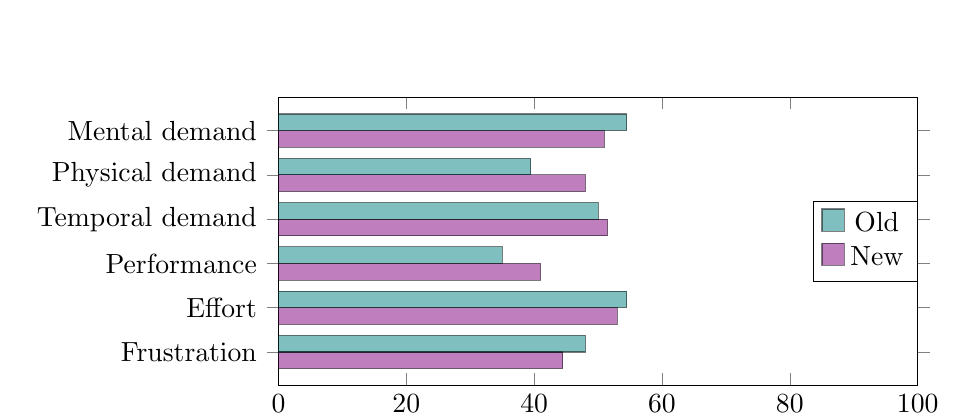
\begin{tikzpicture}
  \begin{axis}[
      width=0.8\columnwidth,
      height=0.8\columnwidth,
      bar width=6pt,
      xbar=0pt,
      xlabel=Mean TLX value,
      y=16pt,
      xmin=0,
      xmax=100,
      enlarge y limits=0.15,
      symbolic y coords={Frustration,Effort,Performance,Temporal demand,Physical demand,Mental demand},
      ytick=data,
      anchor=east,
      legend style={at={(1,0.5)},anchor=east},
      reverse legend,
      ]
  \addplot[fill=violet, opacity=0.5] coordinates {(44.5,Frustration) (53,Effort) (41,Performance) (51.5,Temporal demand) (48,Physical demand) (51,Mental demand)};
  \addlegendentry{New}
  \addplot[fill=teal, opacity=0.5] coordinates {(48,Frustration) (54.5,Effort) (35,Performance) (50,Temporal demand) (39.5,Physical demand) (54.5,Mental demand)};
  \addlegendentry{Old}
  \end{axis}
  \end{tikzpicture}
  \caption{Mean NASA-TLX results for each system. Lower is better.}
  \label{fig:tlx}
\end{figure}

\subsection{Follow-up usage}
The logs from the interface were analysed to see how the participants used
Dialogger during the follow-up stage of the study, to discover which features
were being used, and for how long.

All of the participants continued to use the semantic editor of their own
accord as part of their work. The total time spent by the four remaining
participants (P1, P2, P4, P5) using Dialogger in the follow-up period was 23 hours
and 58 minutes.  Over 14 hours of those were from P2, with P4 using it for 5
hours, P1 for 3 hours and P5 for 20 minutes.

\begin{figure}
\centering
  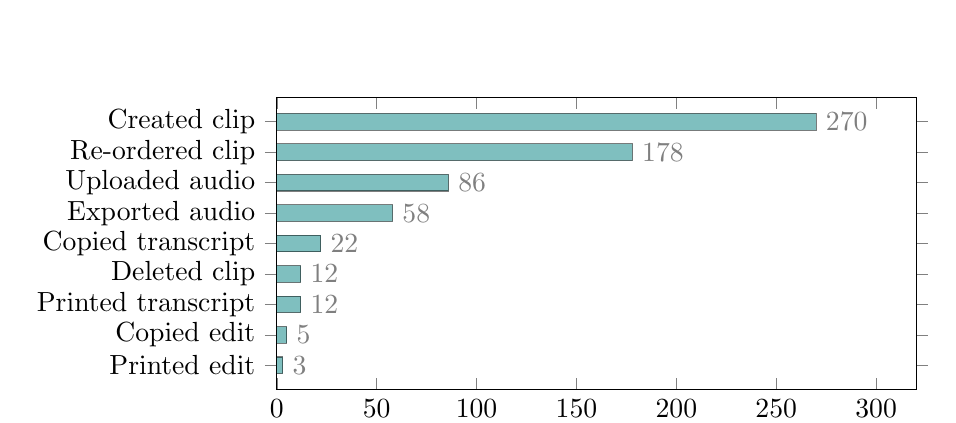
\begin{tikzpicture}
  \begin{axis}[
      width=0.8\columnwidth,
      %height=0.7\columnwidth,
      bar width=6pt,
      xbar=2pt,
      xlabel=User actions,
      y=11pt,
      xmin=0,
      xmax=320,
      symbolic y coords={Printed edit,Copied edit,Printed transcript,Deleted clip,Copied transcript,Exported audio,Uploaded audio,Re-ordered clip,Created clip},
      ytick=data,
      nodes near coords,
      ]
  \addplot[fill=teal, opacity=0.5] coordinates {(3,Printed edit) (5,Copied edit) (12,Printed
    transcript) (12,Deleted clip) (22,Copied transcript)
    (58,Exported audio) (86,Uploaded audio) (178,Re-ordered clip) (270,Created clip)};
  \end{axis}
  \end{tikzpicture}
  \caption{Count of logged user actions during follow-up}
  \label{fig:actions}
\end{figure}

Figure~\ref{fig:actions} shows that over 80 recordings were uploaded and over
50 audio edits were exported. The figure also shows that copying the transcript
was more popular than printing it.

Users could navigate the content by either clicking on the waveform or by
clicking on a word in the transcript. In the interaction log, over 98\% of
navigation actions were executed by clicking on a word, which shows a clear
preference for navigating by text.

%\section{Implications}

%Remove as well as take away

%Annotation is import. Need to include word processing features

%Paper is still used, portable and easy on eyes

\section{Discussion}\label{sec:discussion}
% Others didn't test properly, we did
Previous work on transcript-based media interfaces introduced a range of novel
features for semantically navigating and editing audio and video content.
\citet{Whittaker2004} showed that for voicemail content, semantic editing using
automatic transcripts was faster and as accurate as waveform-based editing.
\citet{Casares2002}, \citet{Berthouzoz2012} and \citet{Rubin2013} all created
similar systems for audio and video production, but they used perfect
transcripts and did not perform any formal studies on the semantic editing
features. In this paper, we presented a semantic speech editor that was
designed specifically for radio producers based on the results of a pilot
study. We studied the existing workflow and evaluated the impact of the
semantic editor through a qualitative study of five professional radio
producers.

% Logging and rough editing is boring
We found that for production of factual radio programmes, a significant amount
of time is spent `logging' speech recordings by transcribing them by hand and
making notes. This process helps the producer to select the best bits of their
material and to structure the narrative of their programme. After logging,
producers create a rough edit by using an audio editor to pick out each piece
of audio they want, guided by the timestamps in their notes. However, these
processes take a long time, require concentration, and are considered to be
boring and tedious.

% Our system was much faster, so frees up their time for other things
Our semantic editing system `Dialogger' introduced automatically-generated
transcripts, which meant that the participants could log their recordings much
faster.  Additionally, the interface allowed them to edit the audio directly
from the transcript, bypassing the rough edit stage, and saving additional
time. Freeing-up this time would allow the producers to concentrate on more
valuable activities such as background research, finding contributors, or
recording additional material. In turn, this could have the potential to
improve the editorial quality of the programme.

% Most of the benefit is from the transcript itself, but how much?
In our experiment, the automatic transcription and the editing interface were
tested as a whole. However, many participants suggested that most of the
benefit derived from the system came from the automatic transcription. A future
study could test these aspects separately to investigate the proportional time
saved by the transcription compared to the interface itself.

% The transcripts aren't perfect, but they're good enough to edit when you can
% listen
As the transcripts were automatically-generated, approximately 16\% of the
words were inaccurate. Despite this, most participants found them to be
sufficiently accurate for their purposes, which supports the findings from
voicemail editing \citep{Whittaker2004} and voice-based discussions
\citep{Sivaraman2016}. 

% Even if the transcript is perfect, producers still need to listen
In theory, if the transcripts were perfect, it would be possible to rough cut
recordings without having listened to them. However, a verbatim transcript
cannot tell you whether something was said seriously or in jest, or about
emphasis, cadence, intonation or background noise. Therefore, an interface that
allows users to edit speech based purely on the transcript carries the risk of
creating poor quality results. It is important for such systems to make it easy
for users to listen to parts of the transcript so they can determine the
quality of the audio they are editing.

% Transcripts need correcting to be readable on their own
Although the automatic transcripts were considered good enough to edit with,
the producers often had to listen to parts of the recording to make sense of
them. If the transcripts are to be used independently of the audio, the
producer must have an easy way to fix the mistakes. Rather than make the user
type out each replacement word, this process could be aided by allowing them to
select alternative words that were rejected by the speech-to-text system.

% Many producers like working on paper, but need to listen to make sense
Despite the importance of listening, many producers like to work on paper.
Participants said that they enjoyed being able to work away from the desk, that
it was easier on their eyes, and that it was easier to collaborate with others
using printed documents. However, when transcripts are printed, the timing
information which links the words to the audio is lost. It would be feasible 
to develop a system for moving between paper and the screen which could
retain this information, but no such existing system could be found.

% Annotation helps the producer to mark their favourite bits
The role of the transcripts is ultimately to help the producer pick which bits
of audio to use in their programme. To achieve this, they use annotations to
mark and rate segments of the transcript. This functionality has not been
considered in any previous semantic editing systems, but we found it to be an
important feature which participants went out of their way to replicate.

In creating and testing Dialogger, we found that there was demand for semantic
editing in radio production. This was backed up by the continued use of the
system during the follow-up period, which was unprompted.
During the study, many of the radio producers reported that a similar
transcript-based workflow exists in television production. Due to the high
costs of video editing, transcripts are often used to make editorial decisions
before editing begins. It would be interesting to see if a semantic video
editor would bring similar benefits to a television production workflow.

% What did you learn from making the system?

% What does this tell us about these kinds of systems?
%- Mature enough to be used in professional practice


% How does this impact the workflow?

% How does this impact the job role?


% Television


% How does this impact the nature of programme making


%CONTIBUTIONS COMPARED TO OTHER WORK

%Logging helps producers to recall what was said in interviews and to structure
%and cross-reference

%Logging takes a long time, requires concentration and is boring.

%Producers annotate the logs with timestamps, notes, highlighting and star
%ratings.

%Word is used and preferred for making annotations

%Navigation using a transcript is considered faster

%There is a desire to listen to the audio faster than real time

%The transcript is accurate enough to do a rough edit

%A more accurate transcript would be beneficial

%The transcript interface is not needed for short recordings or fine editing

%Drag and drop clipping didn't work very well as it's hard to select long bits

%There is a desire for cut and delete functionality

%Working on paper is desirable

%Television could also benefit from this approach

%Need to listen to the audio

%Task completed up to twice as fast with the new system when including logging

%Participants continued to use the prototype after the study

\subsection{Outcome}
Based on the results of this work, we developed the prototype further to add
support for video editing and to take into account the feedback from the
producers in our study.  We handed the prototype over to a development team at
the BBC who have now turned it into an officially supported production tool. We
hope that this will allow producers from around the BBC to use the tool as part
of their normal workflow.

\subsection{Summary of main findings}\label{sec:findings}
%used a pilot study to identify an opportunity to use automatic transcripts of
%dialogue with synchronised audio to connect two previously separate activities
%in radio editing. This had mixed results as shown by the weak stats but more
%positive comments. It exposed some important missing functions like annotation
%and the importance of paper. The exercise also seems to have resulted n the
%first published study of documentary radio production.

% start with a summary and then extend each element at greater length

\paragraph{There is demand for semantic editing in radio production}
In the follow-up stage of the study, all of the participants continued to use
the semantic editing interface of their own accord as part of their production
workflow. This result demonstrates that they find the interface beneficial to
their practice. The interface has also been developed into a supported
production tool which also demonstrates that there is a business case in making
this available to production staff.

\paragraph{Semantic editing is faster for long recordings}
For editing short audio content ($\sim$10 mins), or when editing without
logging, we found that there was no speed benefit in using semantic
editing. However, logging and rough editing longer recordings using the
semantic editing workflow was completed up to twice as fast as the existing
workflow. Participants also commented that the semantic editing system felt
much faster to use and allowed them to quickly search and cross-reference the
material.

\paragraph{Automatic transcriptions are sufficiently accurate}
The participants in the study used automatically-generated transcripts to
navigate and edit the audio. Even though the transcripts had a word error rate
of approximately 16\%, they were found to be sufficiently accurate for the
purposes of radio production.  This supports similar findings about semantic
editing of voicemail content from \citet{Whittaker2004} and of voice-based
discussions from \citet{Sivaraman2016}. However, the more accurate
the transcripts are, the better.

\paragraph{Annotation features are important}
Participants annotated their logs with timestamps and notes, and used star
ratings and highlighting to indicate important parts of their recordings. As
this functionality was not included in the semantic editing interface, some
participants imported the transcripts into MS Word to allow them to make these
annotations.  This demonstrates that annotation is an important feature to
include in such systems.
%This broke the connection between the audio and the text.
%These annotation features could be added to the semantic editing system which
%would allow the audio and transcript to remain linked.

%\subsection{Drag-and-drop doesn't work}
%The interface was designed so that users could select desired pieces of content
%using a drag-and-drop technique. This design worked well for short clips, but
%could not handle long clips. In addition to selecting content they did want,
%participants were also interested in removing content that they didn't want. 
%Enabling word processor style editing like cut, copy and paste would give the
%users more freedom.
%%TODO SO...

\paragraph{Producers want to work on paper}
The participants often used paper to read and annotate their scripts and logs
because it was easier on their eyes, helped them to collaborate and allowed
them to be productive away from the desk, such as in caf\'{e}s and on trains.
During the study, one participant printed the transcript from the semantic
editing interface and worked on paper, even though this meant having to go back
to find and create the desired clips.

%went out of their way to edit on paper by printing and
%highlighting the transcript.  Being able to move between the screen and paper
%would bring the benefits of paper working and allow producers to use their time
%more efficiently.

\paragraph{Listening is important}
Finally, participants pointed out that ``radio is made with your ears''.
Editing decisions are based not only on what is said, but how it is said. This
emphasises the importance of a multi-modal interface, which combines the
efficiency of text-based working with being able to quickly listen back to the
audio.  Enhancing this with faster than real time listening would allow
users to review material at much faster speeds than they do already
\citep{Vemuri2004}.


\section{Conclusion}\label{sec:conclusion}
Semantic editing of speech has direct applications in professional audio
production, but previous studies of such systems were informal and used amateur
participants. We developed a semantic speech editing system based on the
results of a pilot study of radio production, and conducted a formal user study
of the system with five producers at the BBC.  We used speech-to-text to
generate transcripts, which were accurate enough to allow the producers to
rough-edit their recordings up to twice as fast as their current method.
During the study, we discovered that annotating the transcript is an important
part of the editing process, and that producers enjoy working on paper.
Although it is possible to use these systems to edit audio using only a
transcript, we found that it cannot replace listening to the audio. After the
study, the producers continued to use the system, which has since been
developed into a supported BBC production tool after receiving investment.

\section{Future work}
One of our findings was that producers want to be able to work on paper. In
order to facilitate this, we are currently working with a digital pen
manufacturer to develop a semantic editing system that would allow producers to
edit the audio by annotating a printed transcript. 

%As the semantic editing tool becomes part of the normal production workflow, we
%will closely monitor its usage and attempt to measure its impact. We will do
%this by building in metrics and setting up a working group to receive regular
%feedback directly from users.

We found that semantic editing was faster for long recordings, but it would be
interesting to investigate how long a recording needs to be before the benefits
of semantic editing outweigh the costs. Additionally, it is unclear how much of
the speed benefit comes from automatically generating the transcript, and how
much comes from the editing interface.

%In future work, we plan to improve the semantic editing interface by adding
%faster than real time playback, and moving closer to a word processing style
%design that includes cut, copy, paste, delete, undo and annotation features.

%We will also be investigating whether a
%similar system can be achieved on paper using digital pen technology.

Now that our system has been developed into a supported production tool, we
will monitor its progress and record metrics to track its usage. As the
system now includes support for video editing, it could be used to investigate
the benefits and challenges of semantic editing for television production, and
contrast it with those of radio production.

%Semantic speech editing systems allow users to navigate and edit speech-based
%audio or video content using a transcript-based interface.  Previous studies
%have demonstrated the potential of this approach for a variety of applications,
%however the evaluations have all been in a laboratory setting and have mostly
%been informal.  In this paper, we presented the first evaluation of semantic
%speech editing in an uncontrolled environment.

%We conducted a qualitative study of five radio producers at the BBC to discover
%how programmes are made, and to evaluate our semantic editing system. The study
%found that current radio production practice involves spending a lot of time
%logging and rough editing interviews, which is lengthy, requires concentration
%and is considered boring.

%Logging and rough editing interviews using the semantic editing interface was
%up to twice as fast for long recordings, and allowed users to quickly
%search and cross-reference material. Although the automatically-generated
%transcriptions were imperfect, they were considered by participants to be
%sufficiently accurate for their purposes. 

%Annotation features for marking good bits or making notes are an important part
%of the rough editing process. As these features were not available, some
%participants copied the transcript into Word so they could do this. We also
%found that producers enjoy working on paper as it is easier on their eyes and
%allows them to work away from their desk.

%Text-based interfaces allow users to see what was said, but it was noted that
%for producers it is also important to be able to hear how it was said.
%After the study was complete, the participants continued to use the semantic
%editing system of their own accord and it is now being developed into a
%supported production tool.


%TODO
%move to a word like interface with cut, copy, paste, delete and annotation
%create a paper interface

%the paper needs some reflection on the aims and motivation at the end to
%underscore the lessons of the work and say what its contribution is compared
%with existing work

%\begin{itemize}
  %\item The process of logging and rough editing is an important part of radio
    %production, but is slow, boring and requires a high level of concentration.
  %\item Automated transcription is sufficiently good to replace the logging
    %process, but requires an easy way to make annotations.
  %\item Creating a rough edit using a transcript can be less mentally demanding
    %and up to twice as fast.
  %\item The participants voluntarily continued to use the prototype after the
    %study.
  %\item Listening is an important part of producing audio content.
%\end{itemize}

%Next
%\begin{itemize}
  %\item Develop and test method of link paper printouts to audio, perhaps using
    %digital pen technology
  %\item Conduct similar study for TV production
  %\item Develop method for keeping a script in-sync with the audio edit
%\end{itemize}

%%\textit{``There might be a version, a few steps down the track, where you cut
  %%the sound at the edit following along behind.''} (P3)

%A future version could try to
%emulate the word processing actions of highlighting and typing, or using
%context menus.

%The unexpected behaviour experienced in the observation suggests that the
%prototype is missing some desired features, namely the ability to make
%annotations, create a script and to integrate with paper.

%More advanced features could include a rating system for marking how important
%bits are on a scale.


\chapter{Paper-based semantic speech editing}

\section{Introduction}

Digital documents are often reviewed and proofread by printing the document and using a pen to annotate the text. This
approach is still popular, despite the widespread availability of similar functionality in word processors
\citep{Harper2001}.

Working on paper offers a number of advantages over working on computer.  Paper is lightweight, portable and does not
require any power, which allows readers to work anywhere.  It is not back-lit, so is easier on the eyes.
%It can be annotated freely whilst reading.
It can be navigated quickly, annotated freely whilst reading and individual pages can be laid out and easily compared.
Its physical low-tech nature also means that it is intuitive, robust, durable and does not crash or lose data.  These
advantages mean that reading from paper rather than a screen allows readers to gain a deeper understanding, easily
cross-reference other documents, and interleave reading and writing \citep{OHara1997}.

%Transcripts are often printed out because:
%- it is easier to read than on screen
%- allows portability,
%- allows annotation,
%- flexible spatial layout
%- quick navigation
%- cross-referencing,
%- reduces battery anxiety,
%- more trusted by non-tech-savvy users

A similar process happens in the production of media content. The production workflow typically involves recording
material, selecting which parts of that material to use, then editing the desired material down to the final output
\citep{Baume2015}.  Many producers will `log' the material after it is recorded by writing transcripts of what was
said.  This is either done themselves or using a third-party service. These transcripts help producers to recall what
was said and when, identify themes, and make links between different parts of their content.

Many producers find this process easier to achieve on paper than directly on the screen, so choose to print the
transcript. The producer makes hand-written annotations to help them structure their program and make editorial
decisions.  After they have decided which parts they want to use in their programme, they must use audio or video
editing software to manually execute these editorial decisions, which is a tedious and slow process.

In this paper, we describe a system which allows users to edit audio and video content directly using a printed
transcript.  Speech-to-text is used to generate a transcript that has precise timestamps for each word.  The transcript
is printed with an Anoto dot-pattern \citep{Fahraeus2003}, which allows a compatible digital pen to capture annotations
make on the paper.  A digital pen is used to annotate the transcript to mark which parts of the transcript the user
wants to keep or remove.  The audio or video content is then automatically edited to reflect the annotations made on
the transcript.

%The producer prints the transcript then uses
%a digital pen to highlight and strikethrough words to signify the parts they
%want or don't want (see Figure~\ref{fig:layout}). These marks are then
%automatically translated into edit commands by using the timestamps of the
%words to calculate the in-- and out-points for each cut. This produces an edit
%decision list which can be opened in an audio or video editor.

%In this paper, we describe a system which allows users to edit audio and video
%content directly using a printed transcript. Speech-to-text is used to extract
%a transcript with precise timings for each word.
%The digital pen is used
%to select or delete parts of the transcript.

%Our system automatically generates a transcript using speech-to-text. Even
%though it's imperfect, it is good enough to make edit decisions with
%\citep{Whittaker2004}

\section{Related work}
Our system combines editing of media using transcripts with annotation of paper using digital pens. These approaches
have previously been explored individually, alongside related techniques such as navigation of media using paper
transcripts, digital ink annotation of video and paper-based note taking for media.

Transcript-based interfaces have already successfully been applied to both audio and video editing. SCANMail
\citep{Whittaker2002} demonstrated the advantages of navigating voicemail recordings using a transcript, but did not
include editing capabilities.  The LIDS Editor \citep{Apperley2002}, and later TRAED \citep{Masoodian2006}, used
automatically-generated transcripts to allow users to navigate and edit lecture recordings by removing and rearranging
sentences and words. Even though automatically-generated transcripts are imperfect, Whittaker and Amento found they are
sufficiently accurate to allow navigation and editing \citep{Whittaker2004}.  More recently, Rubin \citep{Rubin2013}
created a system for using editable crowd-sourced transcripts to create audio stories.  Similar techniques have been
applied to video editing. SILVER \citep{Casares2002} was a video editor that had an editable transcript window,
generated from subtitles, and Berthouzoz et. al.  \citep{Berthouzoz2012} developed a system that used crowd-sourced
transcripts and image processing to allow text-based editing of multi-camera video interviews.

The Anoto dot pattern can be used with digital pens to bridge the gap between paper and digital documents. PADD
\citep{Guimbretiere2003} was a concept for a system of editing documents that allowed users to move from digital to
paper and back again. ProofRite \citep{Conroy2004} was an implementation of this, which anchored annotations made on
paper into a word processor such that they `reflow' with the text they were attached to.  PaperProof \citep{Weibel2008}
improved on this by interpreting the edit annotations and automatically applying them to the document.

Paper transcripts have been explored as a method of navigating video recordings by using a device to detect the
position in the text and play the video from that position. Video Paper \citep{Hull2003} was a system that embedded
video keyframes with barcodes down the side of the page. It used a PDA to scan the barcodes that linked to a position
in a video, which was downloaded and played on the device. Books with Voices \citep{Klemmer2003} was a similar system
which tested this approach with oral historians who found it had substantial benefits with minimal overhead. Erol et.
al. \citep{Erol2007} went a step further by embedding the video data in the barcode, removing the need for the server.
HotPaper \citep{Erol2008} removed the need for barcodes by using a camera to measure the whitespace between words and
matching that to unique patterns in the text.

Digital ink interfaces on tablet PCs have been explored as a method for annotating and editing video content.  Marquee
\citep{Weher1994} synchronised handwritten notes with a live video recording by using a horizontal line gesture to mark
a timestamp.  Videotater \citep{Diakopoulos2006} was another digital ink interface for segmenting and annotating
pre-recorded video clips. A vertical line gesture on a video timeline split the video, and handwritten words could be
written over a clip. WaCTool \citep{Cattelan2008} extended this functionality by associating user interactions with
edit commands. For instance, users could assign a `skip' command by pressing buttons at the start and end of an
unwanted region.  Video as Ink \citep{Cabral2016} allows users to `paint' video frames onto the tablet interface and
then edit the video by using an `eraser mode' to remove unwanted frames.

Dynomite \citep{Wilcox1997} was a note-taking system that recorded audio synchronously with digital ink handwritten
notes.  Users could highlight segments of the audio by pressing buttons to begin or end a segment. They could navigate
the audio through a screen-based timeline interface which displayed the highlighted regions.  The Audio Notebook
\citep{Stifelman2001} was a similar system that used paper and a physical interface that recorded audio and allowed
users to navigate the recordings using their pen on a scroll bar on the side of the page.  ChronoVis \citep{Fouse2011}
used the Anoto dot pattern to record paper notes during playback of a video. The interface allowed users to click on
the digital display of the handwritten notes to navigate to that position in the video.

These previous studies have approached navigation, editing and annotation of media from five different angles, however
these have yet to be combined.  Our system primarily merges the first two approaches -- transcript-based editing and
annotation using digital pens. In this paper, we will consider this technique in the context of professional media
production.

\section{System requirements}
We informally tested a paper prototype of our system concept on five radio producers from the BBC. The purpose of the
test was to validate our assumptions about annotation of transcripts, gather feedback on which features were valued and
to select an approach of translating annotations to edit commands.  Two of the participants worked in current affairs,
two in science and one in documentaries. The participants had between 7 and 13 years experience working as a radio
producer.

\subsection{Paper prototype}
Each participant was asked to provide an interview they had recently recorded, which was automatically transcribed.  We
used a speech-to-text engine based on Kaldi\footnote{\url{http://kaldi-asr.org}}, trained on subtitled television
broadcasts, to extract a transcript from each recording. In addition to providing precise timings for the start and
duration of each word, the speech-to-text system provides a confidence rating to signify the probability of that word
being correct. A speaker diarization \citep{AngueraMiro2012} algorithm was also run on the content to estimate the
times and identities of when different people are speaking.

\begin{figure}[h]
  \centering
  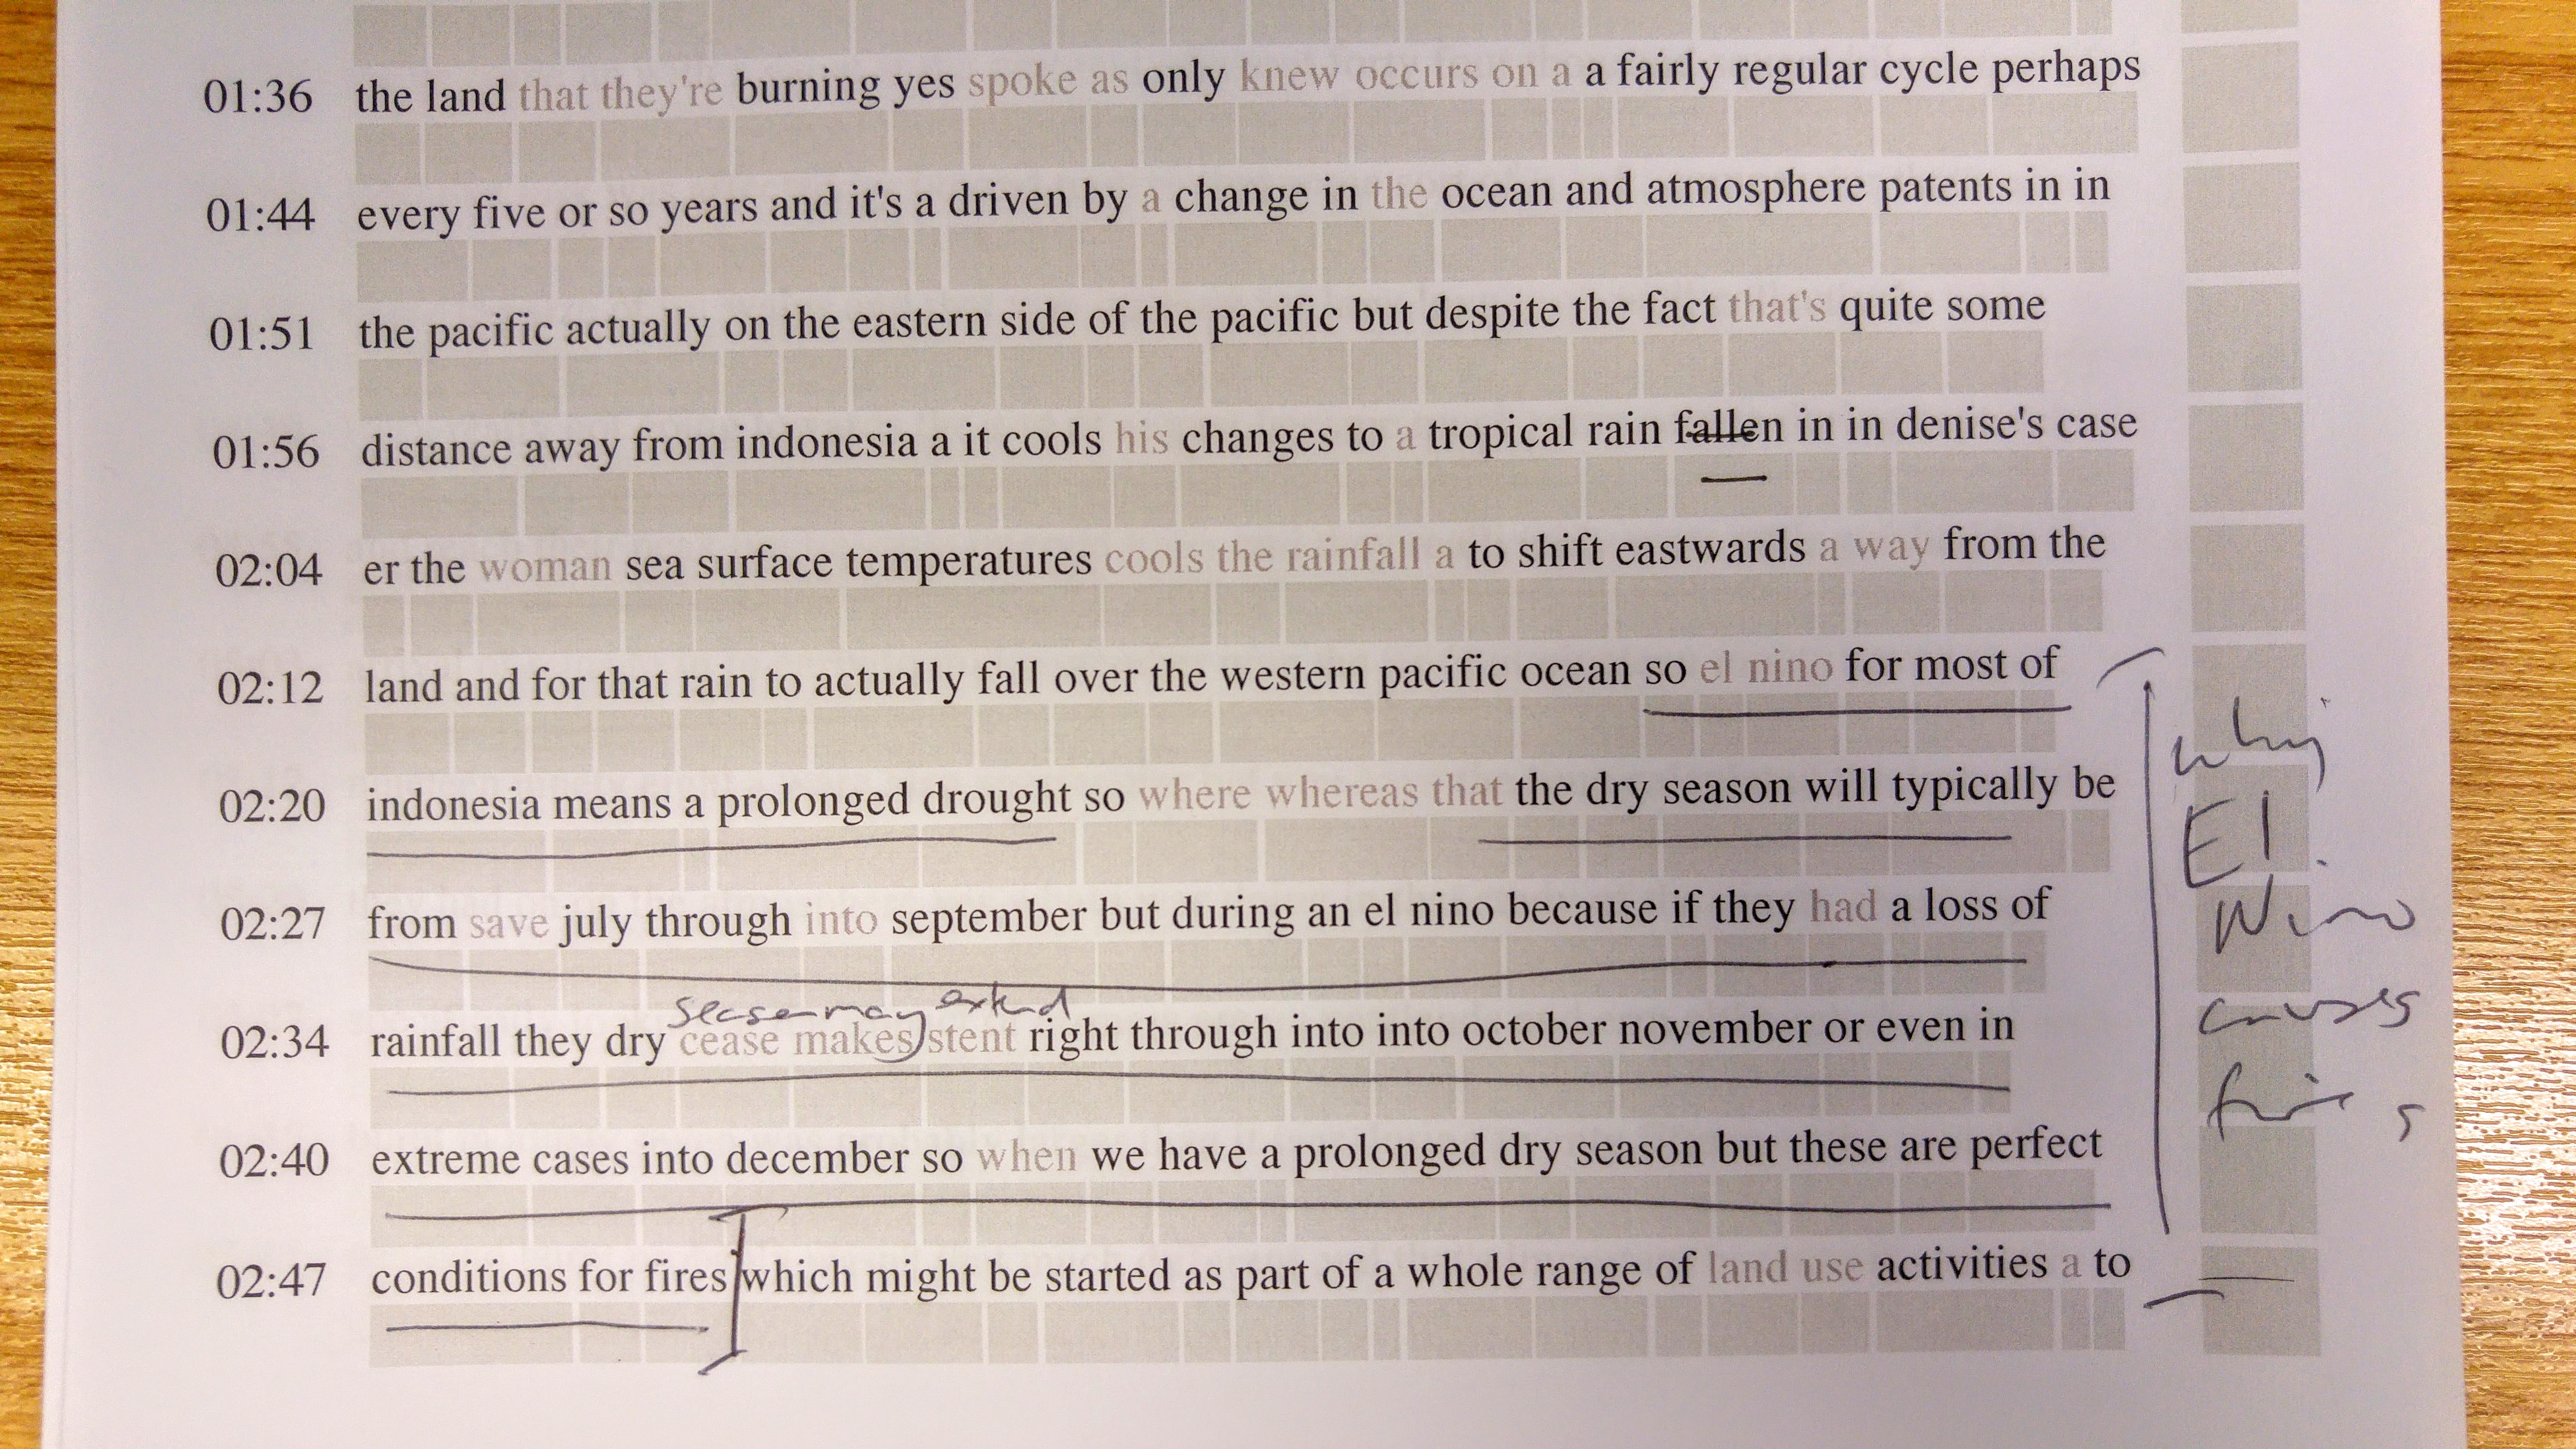
\includegraphics[width=\columnwidth]{figs/mockup}
  \caption{Paper prototype with natural annotations, including
    underlining, line down the side with notes, word corrections, and a
    vertical line to indicate the end of an edit.}
  \label{fig:natural}
\end{figure}

The transcript was printed double-spaced, with a grey box below each word to
indicate the underlining area.  Words with a low confidence rating were
`low-lighted' by shading them grey.  Each line of the transcript had a
timestamp on the left and a square box on the right, which could be used to
select a whole line at a time.

\subsection{Method}
We tested two inactive paper prototypes of the paper interface.
One used the speaker diarization information 
to segment the transcript into paragraphs, with the start of each paragraph
labeled with the speaker identifier in square brackets (e.g.
\texttt{{[}S1{]}}). The other version did not use any of this 
information. The users were presented with the normal transcript first,
followed by the one with speaker information.

For each version, we asked the participants to use a normal pen to annotate the
first page of the transcript as they would normally, to only use strikethrough
on the second page and only use underline on the third page. At the end of the
test, each participant was interviewed about their experience overall and
with each method.

\subsection{Results}
The reaction to the system was overwhelmingly positive. All of the
participants could immediately see the value of such a system and remarked that
it would save them significant amounts of time and \textit{``revolutionise''}
their production workflow.

\subsubsection{Natural behaviour}
The participants started the exercise by annotating the transcript any way they
wanted.  Three of the five participants used underlining to select desired
words, with one using strikethrough to remove words and the other using both
methods.  Three drew a line down the side of the page to select multiple lines
at a time.  Two used short vertical lines between words to signify in- and
out-points for edits.  Two corrected mistakes in the transcript by writing over
or above the incorrect word. Finally, one participant selected words using a
`lasso' technique.

Each participant used a different mixture of annotation techniques. Some of
these techniques, such as underlining, strikethrough and lines down the side,
are easy to detect.  Others, such as corrections, lasso and lines between
words, are less easy to detect. There was no room to write notes at the side of
the page, but one participant did it anyway and two others expressed an interest
in doing so if there was a margin. One participant said that they would
not want a margin.

\subsubsection{Additional features}
Four of the five participants found the paragraphs and speaker information
useful. Typically, interviews have a presenter and contributor and the
producers find it valuable to know when the presenter is asking a question.
Three of the participants said that they were able to find the questions much
more easily with this feature enabled. However, another participant said they
found the speaker diarization \textit{``distracting''}.

All participants found the timestamps and confidence shading features useful,
with some commenting that one timestamp per page would be sufficient.  All of
the participants liked being able to select whole lines at a time, with one
asking whether a similar function could be available to delete content. It was
also suggested that the side boxes could be used to rate or star a selection.

Four of the participants found the transcript was accurate enough to use for
editing their material.  The interview used by the other participant has a
strong Scottish accent which affected the transcript quality. Finally, several
participants noted the importance of listening to the recording and expressed a
desire to hear the content whilst reading the paper transcript.

\subsubsection{Select or delete}
The participants were asked whether
they preferred selecting or deleting words. Three of them preferred select, with
one commenting that it \textit{``felt more natural''} and another saying
deleting felt \textit{``counter-intuitive''}. The other two participants
preferred deleting, with one commenting that it was \textit{``the way my brain
  works''} and the other saying they prefer to \textit{``get stuff out of the
  way''}. As there was no agreement, the system should have options to cater
for a variety of translation methods.

%- Useful to know where presenter is asking question

%Diarization
%- Neal found it easier
  %- Shows where the questions are
%- Phil found it distracting
%- Wes found it absolutely useful
%- Marnie 'made it much easier', liked having paragraphs (usually one point per
%paragraph)


%Timestamps
%needed every couple of minutes

%Use L/R channels for presenter/contributor
%- Phil and Wes
%- Sometimes multiple on R channel (about one in eight interviews)

%Prefer landscape to portrait (landscape is `irritating' and doesn't match
%what's on screen)

%Whole line
%- Would like to delete line at a time

%Note-taking
%- One doesn't take many notes

%Correction
%- One corrects then selects edits
%- Wes would like option

%Highlighting
%- Asterix/star to mark important bits (Phil, Neal)
%- Underline twice (Neal, Marnie liked idea)
%- Wes sometimes double-stars

%Delete vs select (2 vs 3)
%- Phil likes to `get stuff out of the way'
  %- Words that aren't marked should be kept by default
  %- Underline should undo delete
%- Neal prefers selecting over deleting
  %- Delete should undo select, if underlined too far
%- Wes prefers selecting - deleting is `counter-intuitive'
  %- Would like delete to override select, but would like options for opposite
%- Marnie found it trickier to delete than select, selection is more natural
  %- worried about deleting something good
%- Alex feels delete is more natural, 'way may brain works, 'challenge is to
%nibble away', thinks delete should be active, select should override delete

%Margin
%- Phil wouldn't need a margin
%- Neal would like one

%Export
%- gaps should be put between edits (real-time?)

%Transcript
%- Phil and Neal no problems
%- Wes had problems (strong Scottish accent) made it unusable

%Observation
%- Neal
  %- underlined as he read (unprompted), scribbled out when mistake made
  %- found it more difficult to only delete
%- Wes
  %- vertical lines for in/out points

%Other
  %- Neal would like to press and hear word (on laptop?)
    %- Wes: Don't know what sounds good
  %- Wes works in a team of 3/4. They use Box to collaborate

\subsection{Discussion}
%Our system performs the same function as these systems, but uses a paper
%interface rather than a screen-based one.
%Our system
%similarly interprets the paper annotations and applies them to the media
%content.
%Our system does not yet have the ability to replay content from the
%paper interface, but this is a feature that could later be included.
%Our system is based on printed transcripts rather than video frames on
%a tablet, but approaches the same problems from a different angle.
%These systems do not provide the user with any pre-written notes.
%Our system uses speech-to-text to generate a transcript, which the user can
%then annotate further.
The participants used a variety of techniques to annotate the transcripts, 
but underline, strikethrough and lines down the side were common. There were
strong but mixed opinions on whether selection of desired material, or removal
of unwanted material, was the best approach to use for editing, so both should
be made available where possible. However, it is still not clear what should
happen when underline and strikethrough are used together, and which should
override the other.

The transcripts were generated using speech-to-text but were considered good
enough to edit with. We found that participants enjoyed having paragraphs, speaker
information, timestamps, confidence shading and being able to select whole lines.

Some participants expressed a desire to listen to the media
from the paper interface, and this functionality has been shown to be useful
in previous work. Users could start playback by pressing a word with the
digital pen. This could be achieved either by wirelessly
linking the digital pen to a computer that plays the content, or by storing
the audio on the pen itself similarly to the LiveScribe Sound
Stickers\footnote{\url{http://store.livescribe.com/sound-stickers-1-1.html}}.

Previous work has also shown the benefits of being able to write freehand notes
which link to specific points in recordings. These could be attached to a
screen-based interface similarly to ProofRite \citep{Conroy2004}, or handwriting
recognition could be used to store and organise these notes in a structured
way. This approach could also be used to fix incorrect words in the transcript.

Media content is often produced in teams rather than individually.  Although
our system does not prevent multiple people from working on a transcript, it
does not exploit opportunities to smoothly handle multiple users.

We will shortly be conducting a formal evaluation of our system at the BBC
where it will be used to produce audio and video content for broadcast. 

%Providing a function to align an existing script to the recording would allow
%this functionality to be used with scripted programmes.

\subsection{Conclusion}
In this paper, we presented a novel system for editing media content using a
paper-based interface. We tested this concept using a paper prototype in an
informal test on five radio producers.

The participants all reacted very positively to the system. They enjoyed the
additional features we tested including speaker information, paragraphs,
timestamps, confidence shading and selection of whole lines. Based on their
feedback, we also added an optional margin to the interface.

A variety of annotation marks were used by the participants to indicate edit
decisions, including underline, strikethrough, lines down the side and lines
between words.  Participants either preferred to select content they wanted or
to delete content they didn't want, and felt strongly either way.

There are a number of opportunities to build on the system, including being
able to capture freehand notes, listen to the content using the paper
interface, fix incorrect words and work collaboratively.

\section{System design}
Using the feedback from producers, we designed and created a working prototype
of the system (see Figure~\ref{fig:diagram}). To build our prototype, we
collaborated with Anoto who are the manufacturers of the digital pen. We
developed the interface, speech-to-text and media editing, whilst Anoto
handled the transcript printing and translation of the annotations to edit
commands. 

\begin{figure}[h]
  \centering
  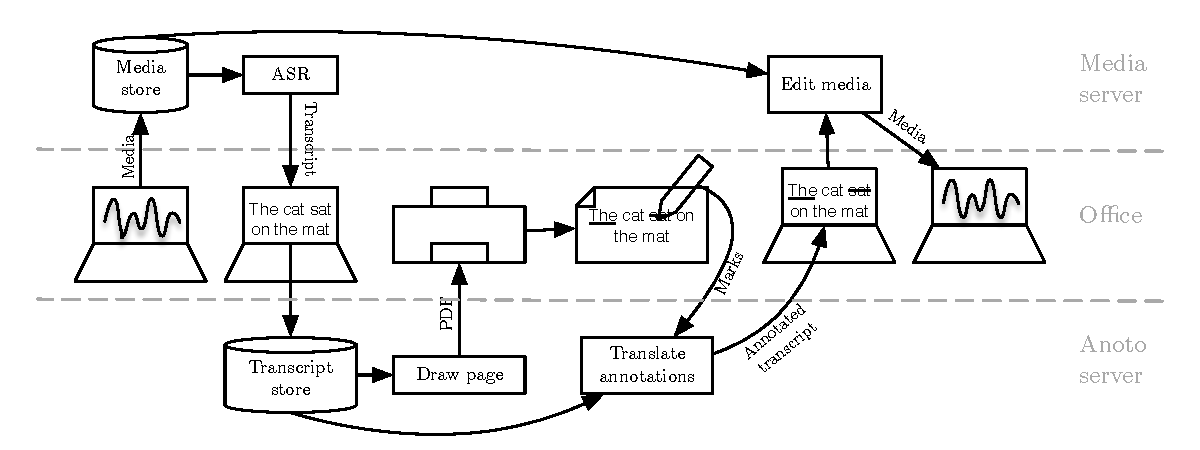
\includegraphics[width=\columnwidth]{figs/uist-sys-diagram}
  \caption{System diagram, flowing from top to bottom}
  \label{fig:diagram}
\end{figure}

Based on the feedback from users, the timestamps, paragraphs, speaker
information and confidence shading have been retained. However the timestamps
only appear at the start of each paragraph. An optional margin has also been
added to allow users to make unstructured notes using their digital pen. 
It is not currently possible to select a whole line at a time, but this will
shortly be added.

For each word in the transcript, two rectangular active areas are defined on
the page -- one around the word itself and another in the space directly below
the word, which is lightly shaded. Any marks made on or below the word label
that word as `deleted' and `selected', respectively. This allows the user to
use a digital pen to delete words using a strikethrough, or to select words by
underlining.  The annotations are automatically uploaded in batch to the system
when the pen is docked.

\begin{figure}[h]
  \centering
  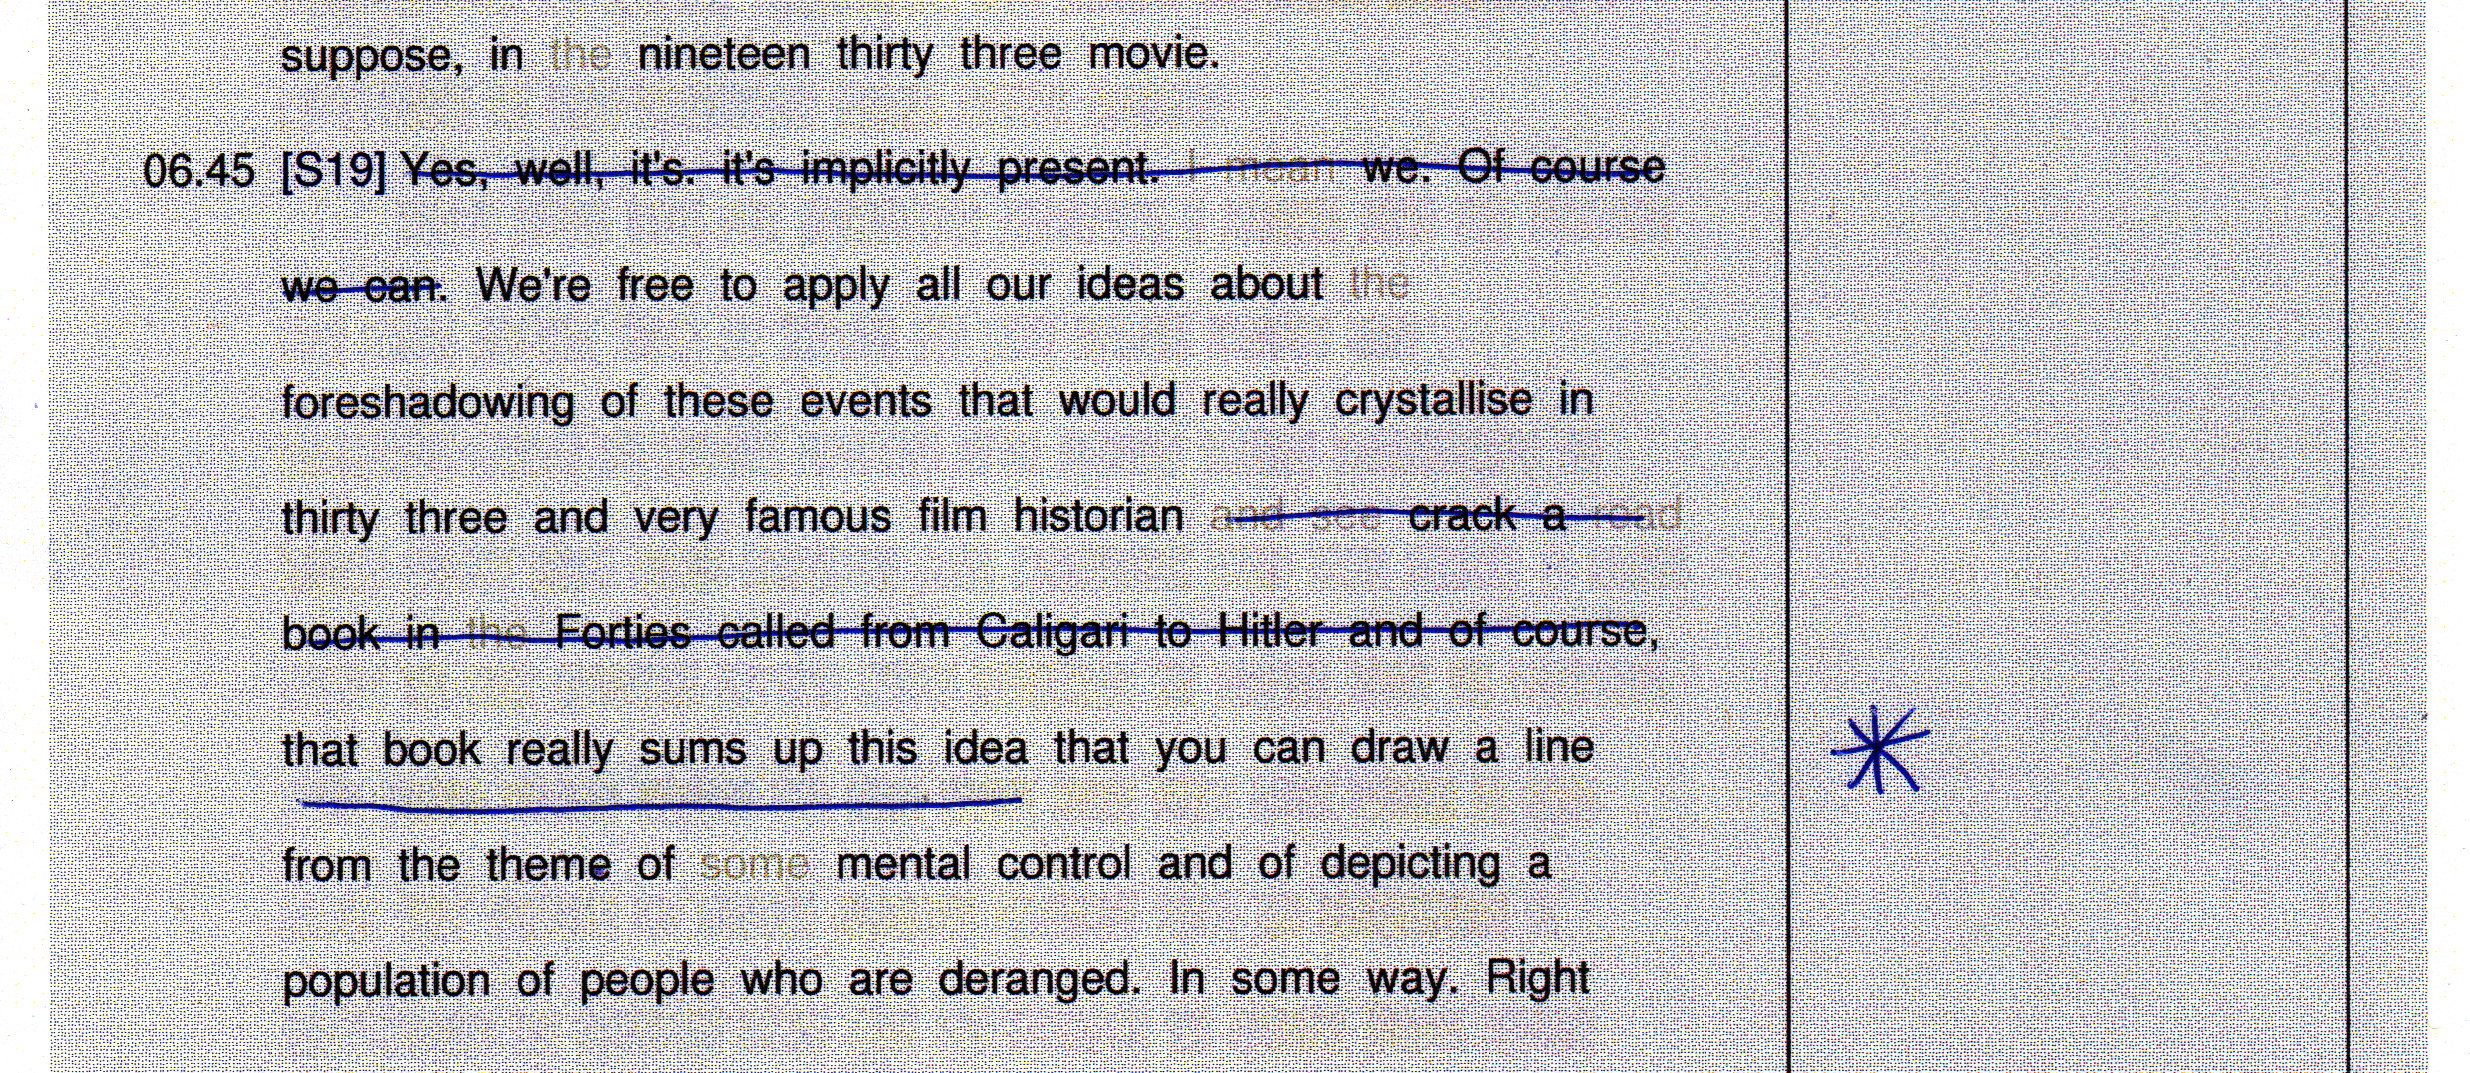
\includegraphics[width=\columnwidth]{figs/interface-darkened}
  \caption{Example of working prototype, showing the shaded box beneath each
    word, paragraph for each speaker with timestamp (06.45) and identity (S19),
    and optional margin for freehand annotations.}
  \label{fig:layout}
\end{figure}

The uploaded annotations are combined with the word timings to calculate the
edit commands.  These can be used to directly edit the media (as shown in
Figure~\ref{fig:diagram}) which removes the unwanted parts of the content. This
is known as a `destructive' edit.  Alternatively, the edit commands can be used
to create an edit decision list (`EDL'). An EDL file describes the in- and
out-point for a series of edits, which can be loaded into audio or video
editing software.  As it is `non-destructive', this approach allows the user to
make corrections to the edit before it is rendered. 

%Several approaches can be taken in interpreting the delete and
%select annotations:
%\begin{itemize}
  %\itemsep0em
  %\item Remove words marked as deleted, except those marked as selected
  %\item Only keep words marked as selected, except those marked as deleted
  %\item Remove words marked as deleted, highlight words marked as selected
%\end{itemize}

\section{Methods}

\subsection{Design and procedure}

% Explain why video recording wasn't used

\paragraph{Stage 1: Training and usability study}
Firstly, the participant will be briefed on the background, objectives and
design of the study as detailed in the protocol.  Should they wish to
participate, they will be asked to read and agree to the consent form.

There are two objectives to the training stage – firstly to introduce the
participant to the prototype system so that they understand its capabilities,
and secondly to test the usability of the interface.

The experimenter will set the participant up on the prototype system, including
giving them access to the web-based interface, giving them a digital pen and
configuring the pen’s docking system. The participant will then receive
training on how to operate the web interface, print out transcripts correctly
and use the pen.

The participant will then be asked to perform a series of typical tasks. The
participant can ask questions and, if they become stuck, the experimenter can
prompt them. However, the experimenter will not give any other directions. The
experimenter will note whether the participant was able to successfully
complete the task and document any problems or confusion experienced during the
execution of the tasks. This process will help to flag any obvious stumbling
blocks.

\paragraph{Stage 2: Observation}

This stage will involve observing the participant editing two pieces of content
- one using the screen-based interface and the other using the paper-based
interface. The order of the observation will be alternated between
participants. The two pieces of content should be similar in nature, but
different so that the participant isn't already familiar with the content.

The observation will be done passively to allow natural interaction with the
system in the participant's normal work environment. The experimenter will sit
beside them making written notes. When the participant has some 'down-time',
the experimenter may choose to ask some questions in order to verify or clarify
something they have observed.

The specific items of interest at this stage include:
\begin{itemize}
\item Editing workflow
\item Tools used
\item Data generated
\item Usability challenges and problems
\item Navigation and edit actions
\item Time taken to complete tasks
\item Unexpected reactions
\item Unanticipated usage
\end{itemize}

The prototype will be configured to electronically log the actions of the
participant, which will help provide insights into usage of the various
features of the prototype.

Software Usability Scale \citep{Brooke1996}
Perceived Usefulness \citep{Davis1989}

With the participant's permission, photos may be taken of paper notes,
annotations or the work environment (see 'data protection' section below).

\paragraph{Stage 3: Interview}
Following the observation stage, the participant will be left with access to
the prototype system for at least a further week. This will give them the
opportunity to use the system as part of their day-to-day work and uncover
issues which may be appear in the observation.

After this period has passed, the participant will be interviewed about their
experience. The primary objective is to compare the two production methods and
extract the advantages and disadvantages of both.

An audio recording will be made of the interview (see 'data protection' section
below). This will allow the participant to speak their mind and allow the
experimenter to give the participant their full attention whilst capturing all
of the provided information.

The questions asked will include:
\begin{itemize}
\item Which aspects of the screen-based system did you / did you not find useful?
\item Which aspects of the paper-based system did you / did you not find useful?
\item Overall, which system did you prefer and why?
\end{itemize}


\subsection{Participants}
To make the most of the principal investigator's position in the BBC,
participants will be recruited exclusively from the BBC. They will be invited
to volunteer by way of email passed around using existing contacts in various
departments that produce speech-based content. 

The nature of the study requires that participants conduct the tasks as part of
their day-to-day job. Therefore, participants will be required to gain
permission from their line manager to take part.

Programmes and producers vary significantly in genre and production techniques.
To take this into account, participants will be recruited so that there is a
representative range of styles.

\subsubsection{Selection criteria}

\begin{itemize}
\item The programme being created should be speech-based.
\item The content of the programme must not contain any sensitive material, as
the transcription will be sent to a third-party for transcription (see 'data
protection' section below).
\item The turn-around time of the programme must be long enough to allow time
to recover from any technical issues without affecting broadcast output.
\item The participant must have permission from their line manager to take part.
\end{itemize}

The study will involve between six and nine participants, depending on how many
meet the criteria. This should uncover over 90\% of usability problems
\citep{Nielsen1993} whilst covering a range of genres and styles, and being a
manageable number given the duration of the experiment.

The study will take place at the participant's own desk at their normal place
of work. As the prototype is web-based, they can use their own computer. There
is a standard configuration for BBC desktop computers, so the environment
should be similar for each participant. Use of display screen equipment is
already covered under the existing BBC risk assessment process.

\subsection{Analysis}

\section{Study results}

\subsection{Qualitative analysis}

% MAIN TOPICS:
% Annotation
% Correction
% Editing
% Listening
% Normal workflow
% Paper admiration/restrictions/waste
% Screen-based working/reading paper
% Transcript accuracy
% Transcript itself


% OTHER TOPICS:
% Collaboration
% Cost
% Custom vocab
% Digital/analogue
% Combining recordings
% Non-linear workflow
% Pen hardwaare
% Working remotely
% Speaker diarization
% Speed
% Structuring thoughts
% Transcription speed
% Translation


\subsection{Metrics}

% Speed

\begin{figure}[h]
  \centering
  \begin{tikzpicture}
  \begin{axis}[
    legend pos=outer north east,
    legend cell align=left,
    xmin=0,
    ymin=0,
    xlabel={Audio length (mins)},
    ylabel={Edit time (mins)}]

  % NORMAL
  \pgfplotstableread{
    X Y
    30 30
    58 43
    32 23
    35 53
    28 35
  }\normaltimes
  \addplot [only marks, mark = *, red] table {\normaltimes};
  \addlegendentry{Normal results}
  \addplot [thick, red] table[
      y={create col/linear regression={y=Y}}
  ]{\normaltimes};
  \addlegendentry{Normal trend}

  % SCREEN
  \pgfplotstableread{
    X Y
    37 24
    61 61
    30 30
    25 49
    26 31
  }\screentimes
  \addplot [only marks, mark = square*, blue] table {\screentimes};
  \addlegendentry{Screen results}
  \addplot [thick, dotted, blue] table[
      y={create col/linear regression={y=Y}}
  ]{\screentimes};
  \addlegendentry{Screen trend}

  % PEN
  \pgfplotstableread{
    X Y
    12 9
    75 56
    31 17
    22 19
    27 27
  }\pentimes
  \addplot [only marks, mark = diamond*, green] table {\pentimes};
  \addlegendentry{Pen results}
  \addplot [thick, loosely dashed, green] table[
      y={create col/linear regression={y=Y}}
  ]{\pentimes};
  \addlegendentry{Pen trend}

  \end{axis}
  \end{tikzpicture}
  \caption{Edit time performance for each editing system}
  \label{fig:penedittime}
\end{figure}

% Usefulness


% Usability




\section{Discussion}

\section{Conclusions}

\section{Future work}


\chapter{Conclusions and further work}


%\begin{appendices}
  %\renewcommand\chaptername{Appendix}
  %\chapter{Service remits and conditions}\label{app:remit}

\paragraph{Radio 1}
``to entertain and engage a broad range of young listeners with a distinctive
mix of contemporary music and speech''

\begin{itemize}
  \item $\geq$ 60 hours specialist music each week
  \item $\geq$ 25 major live events and festivals each year
  \item $\geq$ 250 new sessions each year
  \item $\geq$ 1 hour of news each weekday
  \item $\geq$ 40 new documentaries each year
\end{itemize} 

\paragraph{Radio 1Xtra}
``to play the best in contemporary black music with a strong emphasis on live
music and supporting new UK artists''

\begin{itemize}
  \item $\geq$ 20\% of output is speech-based
  \item $\geq$ 1 hour of news each weekday
\end{itemize}

\paragraph{Radio 2}
``to be a distinctive mixed music and speech service, targeted at a broad
audience, appealing to all age groups over 35''

\begin{itemize}
  \item $\geq$ 260 hours of live music each year
  \item $\geq$ 16 hours of news and current affairs each week
  \item $\geq$ 130 hours of documentaries each year
\end{itemize}

\paragraph{Radio 3}
``to offer a mix of music and cultural programming in order to engage and
entertain its audience''

\begin{itemize}
  \item $\geq$ 40\% of music output is live or specially recorded
  \item $\geq$ 400 live or specially recorded performances each year
  \item $\geq$ 25 new drama productions each year
  \item $\geq$ 30 new documentaries on arts and cultural topics
\end{itemize}

\paragraph{Radio 4}
``to be a mixed speech service, offering in-depth news and current affairs and
a wide range of other speech output including drama, readings, comedy, factual
and magazine programmes''

\begin{itemize}
  \item $\geq$ 2,500 hours of news and current affairs each year
  \item $\geq$ 600 hours of original drama each year
  \item $\geq$ 180 hours of original comedy each year
  \item $\geq$ 350 hours of original documentaries each year
\end{itemize}

\paragraph{Radio 4 Extra}
``to provide speech-based entertainment. Its schedule should include comedy,
drama, stories, features, readings and programmes that appeal to children''

\begin{itemize}
  \item $\geq$ 55 hours of comedy each week
  \item $\geq$ 55 hours of drama each week
  \item $\geq$ 350 hours of childrens programming each year
\end{itemize}

\paragraph{Radio 5 Live}
``to provide live news and sports coverage''

\begin{itemize}
  \item 75\% of output is news and current affairs
\end{itemize}

\paragraph{Radio 5 Live Sports Extra}
``to bring a greater choice of live action to sports fans by offering a
part-time extension of BBC Radio 5 live''

\paragraph{6 Music}
``to entertain lovers of popular music with a service that celebrates the
alternative spirit in popular music from the 1960s to the present day''

\begin{itemize}
  \item $\geq$ 400 hours of archive concert performances each year
  \item $\geq$ 15\% of music is concert tracks and sessions each year
  \item $\geq$ 300 new sessions each year
  \item $\geq$ 10 hours of speech-based features each week
  \item $\geq$ 6 hours of news each week
\end{itemize}

\paragraph{Asian Network}
``to provide speech and music output appealing to British Asians, with a strong
focus on news and current affairs''

\begin{itemize}
  \item Content is approximately 50\% music and 50\% speech during the daytime
  \item $\geq$ 10\% of music is South Asian
  \item $\geq$ 20 hours of language programming each week, including a mixture
    of Hindi/Urdu, English and other regional languages
\end{itemize}


  %\chapter{Startrack interface description}\label{app:startrack}
This section provides details of the most common operations and how they are
achieved in StarTrack.

\begin{figure}[ht]
\centering
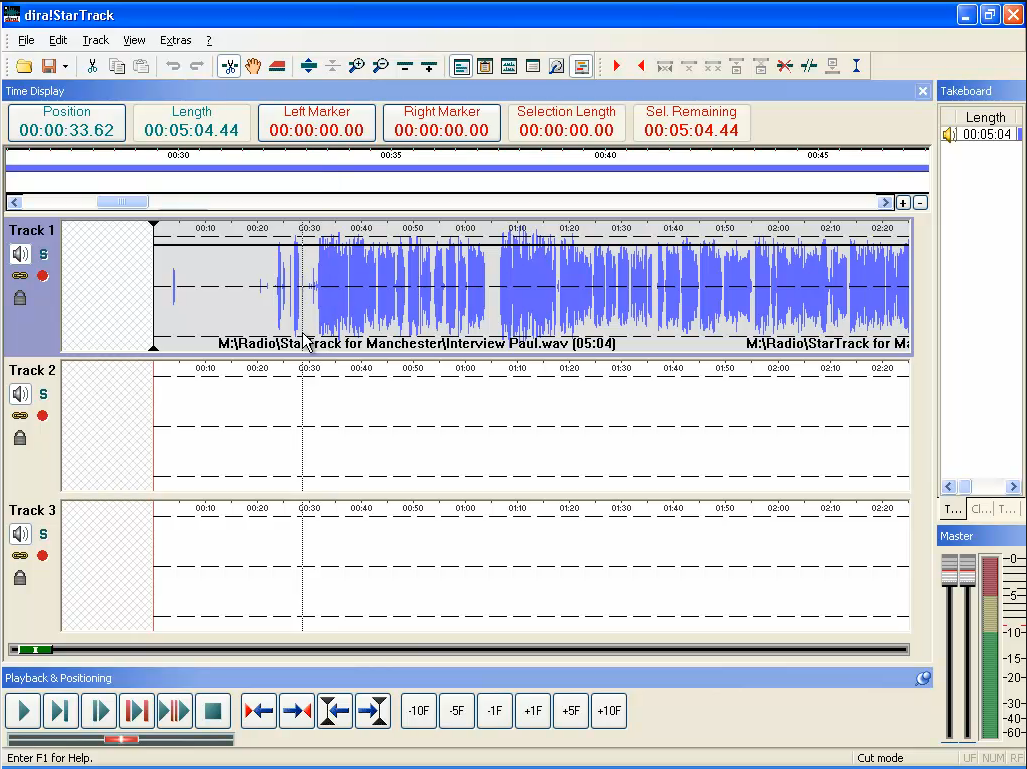
\includegraphics[width=0.8\textwidth]{figs/startrack.png}
\caption{The user interface for StarTrack.}
\label{fig:startrack}
\end{figure}

\paragraph{Modes}
There are three modes in which the StarTrack interface can operate. The default
-- `\textbf{edit mode}' -- is where audio clips can be cut and trimmed,
`\textbf{arrange mode}' is targeted towards moving clips around and
`\textbf{level mode}' is for editing level automation

The primary difference between the modes is the behaviour of the mouse. In
edit mode, clicking the left button sets the position of the cursor, the right
button allows clips to be moved, and dragging with the left button makes a
selection of audio. In arrange mode, the left button selects clips, dragging
moves them around and the middle button sets the position of the cursor. In
level mode, the mouse can be used to move, create and delete nodes in the level
automation.
% what does the right button do?

\paragraph{Playback}
The interface contains five play modes, which were chosen to cater for the most
common editing tasks. They are listed below with their keyboard shortcuts. The
default for $x$ is 2.

\begin{itemize}
  \item \texttt{[space]} Normal playback
  \item \texttt{[B]} Play $x$ seconds from cursor position - used to check
    intro before topping clip. \texttt{[Backspace]} operates in a similar way,
    but with a 5 second lead-up.
  \item \texttt{[V]} Play $x$ seconds up to cursor position - used to check
    outro before tailing clip
  \item \texttt{[N]} Play first and last $x$ seconds of selection - used to
    check selection before clipping
  \item \texttt{[M]} Play $x$ seconds before and $x$ seconds after selection -
    used to check selection before deleting\footnote{This method does not
      perform a crossfade so is not an accurate representation of how an edit
      would sound}
\end{itemize}

The speed of playback can be controlled using the \texttt{[$\uparrow$]} and
\texttt{[$\downarrow$]} buttons, which increases/decreases the rate at which
the audio samples are played (giving a `chipmunk' effect on speech). Pressing
\texttt{[$\downarrow$]} enough times reverses the direction of playback.

\paragraph{View}
The view can be manipluated in a number of ways. The height of the selected
track (vertical zoom) can be controlled with \texttt{[Page Up]}/\texttt{[Page
  Down]}, or by using the mouse to drag the boundaries between tracks. The time
span (horizontal zoom) can be controlled with \texttt{[+]}/\texttt{[-]}, or by
holding \texttt{[Ctrl]} and using the mouse scroll wheel. When some audio is
selected, pressing \texttt{[=]} fits the selection to the window (zoom to
selection).

Each clip has an associated colour and name, which are displayed using the
waveform and a label underneath. These can be changed by right-clicking the
clip and using the context menu.

Markers can be set using the \texttt{[\#]} key and they appear as a triangle at
the top of the track. Each marker has an associated colour and label, although
the label isn't visible. They can be edited by right-clicking on the marker.
Markers are affixed to the audio data, so they remain in place when clips are
copied or moved.

\paragraph{Navigation}
In addition to using the mouse to navigate (as described in the `modes'
section), navigation and selection is aided through the use of a number of
shortcuts:
\begin{itemize}
  \item \texttt{[$\leftarrow$]}/\texttt{[$\rightarrow$]} Move to the
    previous/next edit point or marker. Use with \texttt{[$\Uparrow$]} to move
    to beginning/end of selection.
  \item \texttt{[Home]/[End]} Select to start/end of clip. Use with
    \texttt{[Ctrl]} to move the cursor
  \item \texttt{[7]/[8]} Nudge/nibble the start of the selection left/right
  \item \texttt{[9]/[0]} Nudge/nibble the end of the selection left/right
  \item \texttt{[ / ]} Set in/out markers for selection while playing
\end{itemize}

\paragraph{Editing}

\verb$[\]$ splits a clip into two at the point of the cursor. A solid line
shows that the clip is not connected, and the two parts can be moved freely.

\texttt{[Delete]} removes a selection of audio from a clip and joins the two
remaining parts of the clip together with a crossfade. The edit is shown as a
dotted line with an empty triangle at the top, indicating that the two
remaining parts are connected and move together. The user can undo the edit at
a later stage by right-clicking the triangle and selecting `undo edit'.

\texttt{[w]} removes the selected audio, but separates the remaining two parts
into individual clips and leaves a gap in the middle.

Fade in/out operations must be done using the mouse. There is a triangle in the
top left/right corner of each clip which, when dragged, applies a fade in/out.
It can also be done by making a selection and using the context menu, which has
three curve options.

When clips overlap on a track, their output is played simultaneously. Any
crossfading between the two must be done manually by using level automation.

\paragraph{Levels}
By default, each clip displays a solid horizontal black line which represents a
0dB gain for that clip. It can be moved up and down with the mouse in edit
mode. Holding \texttt{[Ctrl]} changes the level only in the selected region and
holding \texttt{[$\Uparrow$]} affects all of the clips in that track.

Switching to level mode allows finer control using level automation. Nodes can
be created by dragging the first/last node in a clip, or holding
\texttt{[Ctrl]} while clicking on the black line. Nodes can be deleted by
holding \texttt{[Ctrl]} and clicking on an existing node.

\paragraph{Takeboard and clipboard}
The `takeboard' is a list displayed on the right of the interface which
contains a list of all raw audio recordings that are available. They can be
dragged and dropped onto a track.

The `clipboard' contains a list of clips. In this context, a `clip' is a copy
of an edit, which can be made by highlighting part of a track and pressing
\texttt{[C]}. The clip will include any level automation and can include parts
of multiple audio files and silences. In that respect, it can be considered to
be a mini EDL. Deleting a clip does not destroy any raw audio data.

The list of clips can be reordered, and by selecting multiple clips from the
list and dragging them onto a track, they will be inserted one after the other.
This functionality is useful for putting together a rough edit.  Pressing
\texttt{[P]} will preview the selected clip in a small preview window. The
preview only contains play, stop and scroll functionality, but audio can be
selected and dragged onto a track. Clips can be `bounced down' to an audio file
using the context menu.

\paragraph{Slips and chains}
When audio clips (or parts of clips) are removed\slash inserted\slash moved,
the clips to the right of the edit on that track are automatically moved to
fill/accomodate the edit. When multiple tracks are used, this can cause tracks
to fall out-of-sync with each other, but this can be fixed by using either
chaining or slipping.

Chaining is where multiple tracks are grouped together so that when audio is
removed\slash inserted\slash moved, all of the clips on the chained tracks move
together.  When audio is selected on a chained track, it is selected across all
of the chained tracks.

Slipping is similar to chaining but affects all tracks, not just those chained
together. StarTrack provides the option of `right slip', where clips on every
track to the right of the edit move together, or `left slip' where the clips to
the left of the edit move together. Both can be used at the same time, which
gives the effect of chaining all tracks.

Tracks can also be locked so that they are unaffected by actions in other
tracks. This is useful for content such as background music, which doesn't need
to be in sync.

\paragraph{Signal processing}
StarTrack includes support for VST audio effect plugins. A number of
VCS-branded plugins are supplied as standard, including ones for dynamics,
parametric EQ, graphic EQ and mixing. A simulated PPM meter is also available
for checking levels. However, the VST support in StarTrack is currently limited
to VST v2.0, can only support stereo signals and doesn't support channel
mapping. Parametric EQ can also be applied to clips individually through a menu
option.

\paragraph{Saving and bouncing down}
Projects can be saved either `without audio', where the audio data remains
stored in the dira! system, or `with audio', where the audio is copied onto the
local machine. BBC best practise stipulates that the audio should be stored on
dira! whenever possible in order to avoid data loss and to make the files
available to other staff members.

StarTrack performs a local background autosave every two minutes where projects
can be restored through a menu option. When a project is `bounced down' to an
audio file, only the tracks which are visible in the interface are included in
the mix. This can be useful for easily excluding tracks, but is usual behaviour
for a DAW, so could catch people out.

  %\section{Consent form}\label{app:consent}
You are invited to participate in this research study examining the performance
of audio waveforms. The purpose of this page is to provide you with information
required for you to make an informed decision regarding participation in this
research.

\paragraph{What you will be asked to do}
If you agree to participate in this experiment, you will be presented with a
sequence of nine audio recordings and asked to select the music within each
recording. The audio waveform will change throughout the experiment and you
will be asked to rate the performance of each. At the end, you will be asked to
compare them.

It is anticipated that the entire experiment will take between 10 and 15
minutes. You can complete the experiment at a time and location that is
convenient to you. You can also save your progress by creating a bookmark and
completing the experiment at a later date.

\paragraph{Voluntariness}
Participation in this study is voluntary. You may refuse to participate, refuse
to answer any questions or withdraw from the study at any time without any
consequences to you. If you wish to withdraw from the study after having
completed the task, you can do so by sending the ID code below, along with the
request to have your responses removed, to the researcher within 24 hours of
completion.

Your ID code is xxxxxx.

\paragraph{What information will be collected}
{\singlespacing
\begin{itemize}
\item Your browser and OS details
\item Your demographic information
\item Your actions during the tasks
\item Your ratings of the tasks and waveforms
\item The date/time you completed the tasks
\end{itemize}
}

\paragraph{Confidentiality}
No personally identifiable information will be collected during the experiment.
The data and results of this study may be published, but in no way that will
allow you to be identified.

\paragraph{Conditions}
To participate in this study your vision and hearing must be unimpaired and you
have to be at least 18 years old. There are no known or anticipated risks or
discomforts associated with participating in this study. You will not be
monetarily compensated for your participation in this research.

\paragraph{Further information}
If you require any further information regarding this research project or your
participation in the study you may contact Chris Baume
(\url{chris.baume@bbc.co.uk}).  The results of the experiment will be made
available on the following website:
\url{http://www.bbc.co.uk/rd/projects/audio-visualization}

\mbox{}\\
\noindent
\textbf{"I, the participant, have read the above information and wish to
  participate in this study"} [Agree/Disagree]

  %\section{BBC radio production workflow}\label{sec:production}
BBC radio is a huge operation with 59 radio stations spread across the UK
covering every type of programme and music genre. Successfully documenting the
entire system would be difficult if not impossible as different groups and
departments have wildly varying ways of accomplishing the same task.

This section aims to provide a high-level overview of the most common
processes, systems, interfaces and language used in BBC radio production. It
will provide some context to the real-life environment for which the work in
this project will eventually feed into, and may help guide the direction of the
research.

\subsection{Roles}\label{sec:roles}

\paragraph{Producer}
Most radio programmes have one producer who `owns' that programme.  In many
cases, about 80\% of the time spent creating the production is done so by the
producer. In addition to controlling the editorial content, they usually make
the audio recordings and do most of the audio editing. Producers usually only
receive half a day of official training with the rest learnt `on-the-job'.

\paragraph{Presenter/Reporter}
The presenter is the voice of the programme. They provide the links and conduct
interviews with the contributors. In some cases, they work closely with the
producer on the editorial content.

\paragraph{Journalist}
This role is more common in the News division, and the role is usually a
combination of producer and presenter. The emphasis for journalists is on
newsgathering.

\paragraph{Editor}
Editors are senior producers who have a significant amount of experience. They
provide editorial guidance to producers and are often involved with the
programme compliance.

\paragraph{Studio Manager}
The studio manager is responsible for the audio output of the programme. Often
they only get involved at the very end of a production to clean up any rough
edits and apply noise reduction/EQ. In live productions, they operate the
mixing desk and set up remote contributions. In News, senior studio managers
are called Studio Directors.

%\subsubsection{Commissioner}
%When a producer has an idea for a programme, they pitch that idea to a
%commissioner who then decides whether it gets made.

%\subsubsection{Broadcast Assistant}

\paragraph{Media Manager}
Ingests video and audio content for News by setting up ISDN links and BNCS
routing, creating clips from incoming feeds and attaching basic metadata.

\subsubsection{Political structure}\label{sec:organisation}
BBC radio output is produced across three top-level divisions - Radio (formerly
called Audio \& Music), News and North. The structure is listed below.

\begin{itemize}
  \item Radio
  \begin{itemize}
    \item Radio 1, 1Xtra
    \item Radio 2, 6 Music, Asian Network
    \item Radio 3
    \item Radio 4, Radio 4 Extra
    \item Production
    \begin{itemize}
      \item Factual
      \item Arts, Documentaries and Drama
    \end{itemize}
    \item Live Music, Events and Popular Music
  \end{itemize}
  \item News
\end{itemize}

\subsubsection{Services}
The BBC broadcasts a diverse range of speech and music content across genres
including news, drama, comedy, live events, magazine shows, documentaries,
cultural programming and childrens. Quantifying the proportion of these types
of content is difficult as there is little metadata or publications that go
into that level of detail. However, the BBC Trust publishes an annual radio
service
licence\footnote{\url{http://www.bbc.co.uk/bbctrust/our_work/services/radio/service_licences.html}}
which sets aims and objectives for the content of each network. The remits also
include specific conditions which can significantly affect the audio content
(e.g. ratio of music/speech). Using these, it is possible to gauge the
character of each radio network and at least a minimum level of different
content types. The remits and conditions are listed in
Appendix~\ref{app:remit}.

Six of the networks are characterised as a mix of music and speech, with the
other four being purely speech-based. This demonstrates that much more
speech-based audio content is broadcast than music. Of the speech content, much
is likely to be news and current affairs as all of the networks include it to a
greater or lesser extent, and two networks are dedicated to it. With music,
there are a number of conditions that encourage or demand live music and
performances, although the majority of music output will be recordings.

\subsection{Technology}\label{sec:workflow}
The audio workflow at the BBC is vast and complicated. Despite attempts to
harmonise production tools, the wide variety of requirements from production
staff around the BBC means that no one tool can cater for everyone. For
example, some content is turned around in a few minutes whilst other content
could be worked on for a month. However, even though there are plenty of
options available, on a day-to-day basis most producers get by using only the
dira! system.

It would be impractical to capture every single component that audio content
touches at the BBC, so this report will only attempt to detail the most common
systems.  Figure~\ref{fig:workflow} shows a typical audio data flow for radio
production in the BBC.

\begin{figure}[ht]
\centering
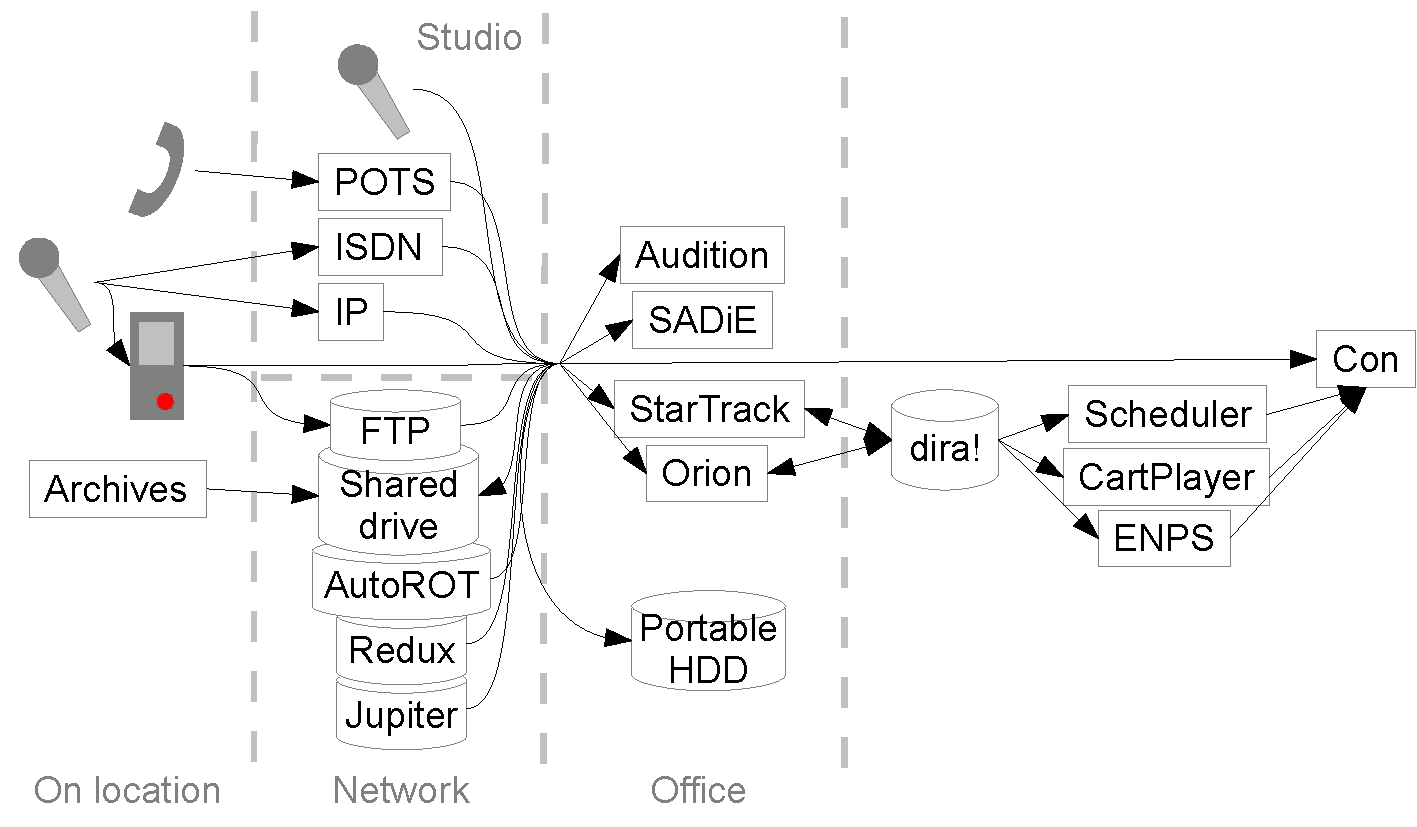
\includegraphics[width=\textwidth]{figs/workflow.pdf}
\caption{Typical flow diagram for audio data in BBC Radio.}
\label{fig:workflow}
\end{figure}

\subsection{Ingest}\label{sec:ingest}
The chosen method of capturing audio content is highly dependent on the type of
programme that is being made. For instance, phone-in shows will combine live
studio recordings with telephone links, and news reports will primarily use
portable recorders. 

\paragraph{Studio recordings}
An obvious but important source of audio content is studio recordings. A
typical set-up consists of an acoustically isolated studio containing a number
of microphones. The studio is connected via triple-glazed windows to one or two
acoustically treated cubicles housing a mixing desk and monitors. The presenter
and guests sit in the studio and the studio manager and producers sit in the
cubicle.

\paragraph{Telephony}
POTS\footnote{Plain old telephone service -- standard phone line} is still used
heavily as it is often the only practical method of setting up remote
contributions on short notice or to members of the public (such as for Radio
4's `Any Answers?' programme).  Where a contribution is planned in advance, an
ISDN\footnote{Integrated Services for Digital Network -- 128kbps digital phone
  connection} link can be set up to a local studio, or to a location equipped
with a ISDN codec box (such as stadiums). This gives a much higher sound
quality but can be expensive if a connection is not already in place.
Increasingly, Internet protocol (IP) links are being used for remote audio
contributions.  Skype is readily used in place of POTS due to its higher sound
quality, and hardware from Comrex (such as its ACCESS and BRIC products) is
being increasingly used to provide high quality contribution links.

\paragraph{Portable recorders}
Recordings made on location are most often made with a microphone and portable
recorder\footnote{Sometimes referred to as a `Nagra' -- a popular brand of
recorder}. The audio, which is stored on Compact Flash or SD cards, is then
either physically taken back to the office or transferred over the Internet
through the use of an FTP server or a browser-based online service provided by
Arbor Media, which automatically copies the recordings into dira!.

\paragraph{Simulrec}
This is a common technique which is used to increase the sound quality of
conversations between a presenter in the studio and a contributor on the
telephone. The interview is conducted over the phone, but each side of the
conversation is also recorded locally using broadcast quality microphones. In
the studio, the recording is made using an audio editor. The contributor is
recorded with a portable recorder and the recording is sent over the Internet
to the studio, where it is imported and lined-up in the audio editor. The
result makes it sound as if the conversation happened in the same room.

\paragraph{Archive} Many programmes require the use of previously-broadcast
material which is stored in one of many archives.

\paragraph{AutoROT} Automatic Record of Transmission (see
Figure~\ref{fig:autorot}) is a popular system that records all network radio
output, plus a number of other streams including the feed from the House of
Commons.  Some of its content stretches back as far as November 2006.  It is
accessed using an online GUI which allows users to audition, clip and download
content.  AutoROT contains a mixture of uncompressed .wav recordings, which are
suitable for re-use, and data-compressed recordings, which are only suitable
for research/browsing.

\paragraph{Jupiter} BBC News store all of their video content in the Jupiter
system, which can be accessed through an online web interface called Davina.
Although not designed specifically for audio content, Jupiter is often used to
take audio data from video recordings.  It is possible to edit audio using a
video editor with Jupiter, but often it is easier to copy the audio content to
dira! and use a program like StarTrack.

\begin{figure}[p]
\centering
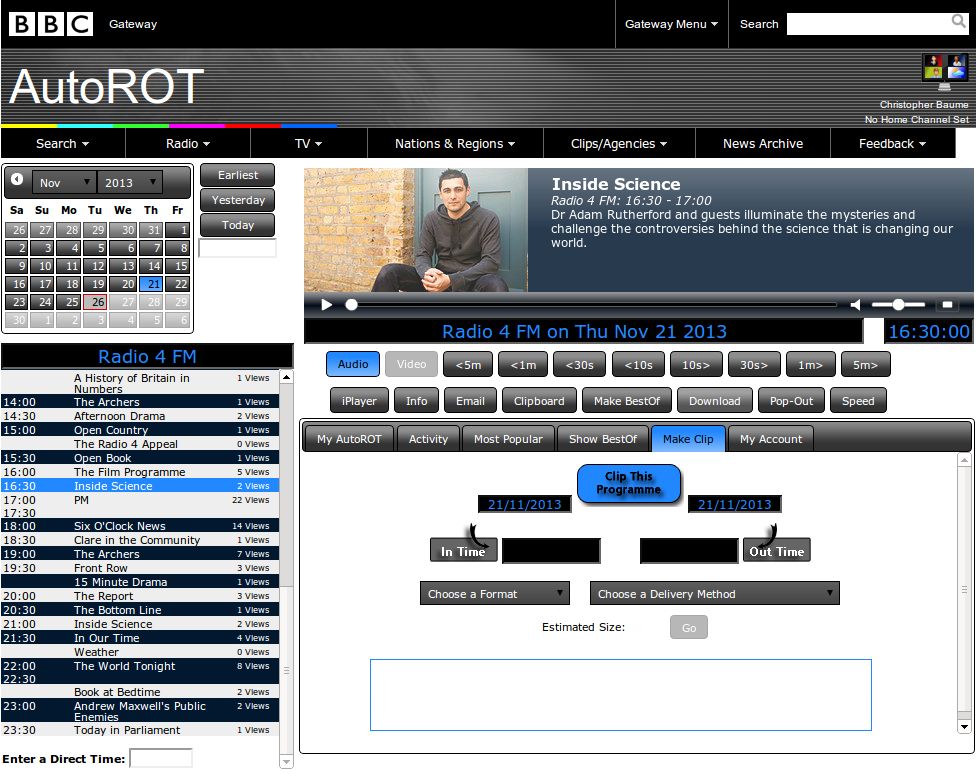
\includegraphics[width=0.8\textwidth]{figs/autorot.png}
\caption{User interface for BBC AutoROT.}
\label{fig:autorot}
\end{figure}

\begin{figure}[p]
\centering
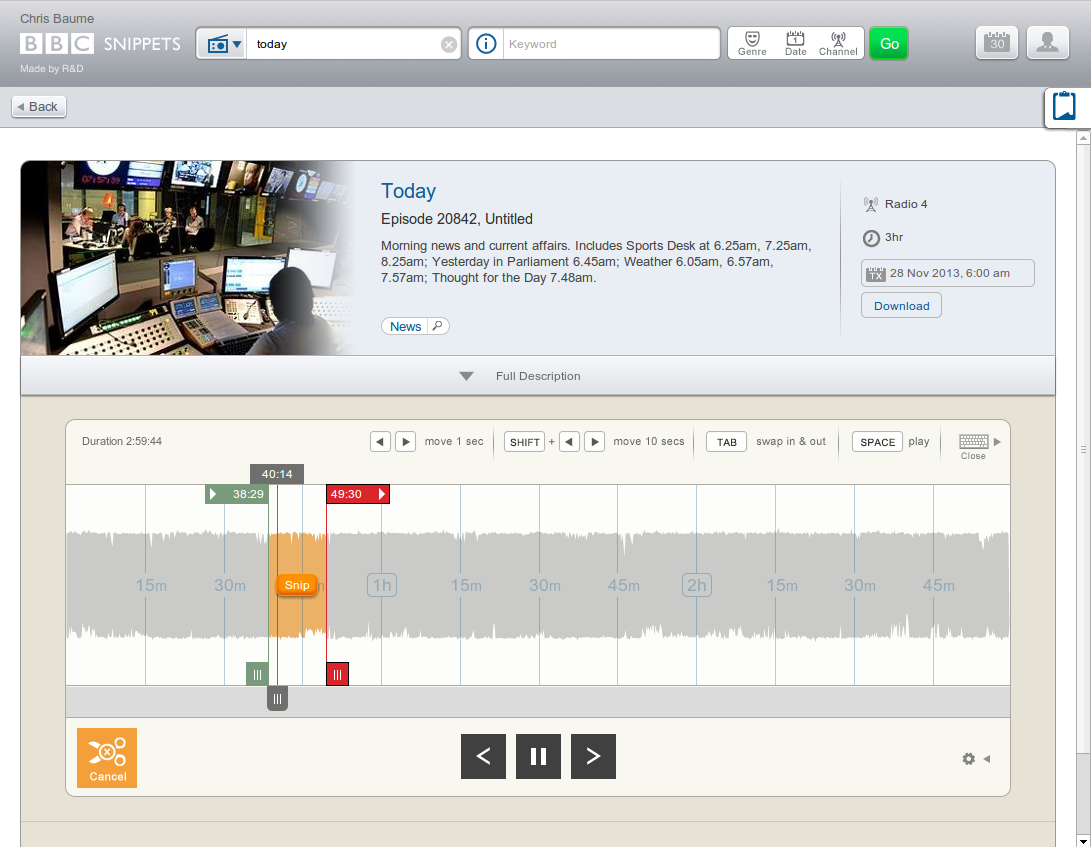
\includegraphics[width=0.8\textwidth]{figs/snippets.png}
\caption{User interface for BBC Snippets for Radio.}
\label{fig:snippets}
\end{figure}

\paragraph{I\&A catalogue}
The BBC's physical archive is managed by the Information and Archives
department, who are primarily based in Perivale. Material can be either be
searched for using the legacy INFAX system or through the new Fabric platform,
both of which are browser-based. Material is found using text-based search
and is then ordered via a phone call. The recording is then either digitised
and deposited in a shared network drive, or the physical media is sent to the
producer via internal mail.

\paragraph{Radio Digital Archive}
The Radio Digital Archive (RDA), and its predecessor the Radio Interim Archive
(RIA), capture all network radio output in uncompressed PCM format. The RIA
started in August 2008 with the RDA taking over in March 2013. They contain
recordings of transmission, pre-recorded items, extended interviews and music
sessions. The RIA stores content as .wav files segmented into 30 or 60-minute
chunks. The RDA uses information from Coyopa (see Section~\ref{sec:coyopa})  to
segment the audio at programme boundaries and to include programme metadata.

\paragraph{Redux}
BBC Redux is an experimental system run by BBC R\&D which records all BBC
television and radio output. It has been running since July 2007. It differs
from other ROT systems in that it records content off-air (via FreeSat). As the
content is data-compressed, it is not fit for broadcast and only used for
programme-making when other archives have been exhausted.

\paragraph{Snippets}
In 2012, a new user interface was developed to allow advanced search and
navigation of Redux. The project, named Snippets, adds features such as the
ability to search the text of television subtitles, audition, clip (`snip') and
download content in-browser and search by cast/crew. The recently introduced
`Snippets for Radio' allows users to navigate radio content with a waveform
display and keyboard shortcuts (see Figure~\ref{fig:snippets}). The code which
powers Snippets for Radio has been open-sourced\footnote{See
  \url{http://waveform.prototyping.bbc.co.uk}}.

\subsection{Storage}

\paragraph{dira! Highlander}
The dira! radio production system is central to the BBC's operation. Almost all
non-live audio content is stored, edited and played out using the system. Dira!
was originally manufactured by a company called \textbf{VCS}, which was then
bought in 2012 by SCISYS. However, within the BBC almost everybody refers to
the dira! system as VCS because of the branding on the software and equipment.

The Highlander program is the user interface for accessing the dira! database
(see Figure~\ref{fig:highlander}). The entire dira! system spans a number of
servers, but Highlander can access only one at a time. Each server consists of
a folder structure where each folder contains a number of `\textbf{stores}'.
The stores contain a `\textbf{take list}' consisting of audio recordings and
StarTrack EDLs\footnote{Edit Decision Lists}.

\begin{figure}[p]
\centering
\includegraphics[width=0.9\textwidth]{figs/highlander-interface.png}
\caption{User interface for dira! Highlander.}
\label{fig:highlander}
\end{figure}

Although the stores are technically identical, they are manually arranged to be
used for different purposes, such as:
\begin{itemize}
  \item \textbf{Programme stores}, for regular programmes (such as Woman's
    Hour)
  \item \textbf{Generic stores}, for other programmes in a given network (such
    as Radio 2)
  \item \textbf{Music stores}, for storing music tracks
  \item \textbf{Recording stores}, for raw studio recordings, recordings of
    transmission and presenter links
\end{itemize}

Each store has an individual capacity and expiration time, after which items
are moved to a `\textbf{recycle bin}'. The recycle bin has a 72 hour expiry
time, after which items are unrecoverable. The capacity/expiration parameters
vary for each store, depending on its use. For instance, stores for regular
programmes expire after 30 days, whilst the music stores never expire.

\begin{figure}[p]
\centering
\includegraphics[width=0.9\textwidth]{figs/audition-interface.png}
\caption{User interface for dira! Highlander audition window.}
\label{fig:highlanderaudition}
\end{figure}

Each audio item has a yellow speaker icon which brings up an audition window
(see Figure~\ref{fig:highlanderaudition}) for playing and navigating the clip.
No editing facilities are provided, but there is a button for sending the audio
clip to the StarTrack editor.

Edit decision lists (EDLs) have a folder icon with the letter `A' associated
with them. When selected, they can be opened with the `send to editor' button.

\begin{figure}[p]
\centering
\includegraphics[width=0.8\textwidth]{figs/take-data-card.png}
\caption{Take data card window in dira! Highlander.}
\label{fig:takedatacard}
\end{figure}

Double-clicking on an item opens the `\textbf{take data card}' or `TDC' (see
Figure~\ref{fig:takedatacard}) which is used to read and enter metadata. Some
fields are compulsory and are highlighted in red, and the others are filled in
subject local conventions. There are different types of TDCs for different
types of content. Those which store audio content are called `\textbf{DIGA}s'. 
% explain what EXTA is

\begin{figure}[p]
\centering
\includegraphics[width=0.8\textwidth]{figs/highlander-filter.png}
\caption{Take list filter window in dira! Highlander.}
\label{fig:highlanderfilter}
\end{figure}

Items can be found by browsing the take list, which can be sorted by title,
duration, time of creation/last modification and username of creator/last
modifier amongst others. The items in the take list can be filtered by text
search, including wildcards (see Figure~\ref{fig:highlanderfilter}), or the
whole server can be searched at once with the results appearing in a separate
window.

\begin{figure}[p]
\centering
\includegraphics[width=0.8\textwidth]{figs/ats-recorder.png}
\caption{The user interface for ATS recorder in dira! Highlander.}
\label{fig:atsrecorder}
\end{figure}

Audio can be ingested into Highlander by importing a file, making a live
recording or ripping a CD. Imported files are normalised before being uploaded
to the database. The live recordings are made using the `\textbf{ATS recorder}'
program. The interface (see Figure~\ref{fig:atsrecorder}) includes a VU meter,
simple faders, and a button for creating markers. CDs can be extracted using
the CDExtract program, which automatically grabs the CD metadata from an
external database.

\paragraph{Shared network drive}
Audio content is often stored in Windows network fileshares which are mounted
as part of the standard IT infrastructure. Until recently, audio content was
stored in a share mounted as `M:' and known as the `M drive'. This has recently
been replaced with a share mounted as `S:'. The `S drive' is is a disaster
recovery server whose data is split across three sites. Broadcast critical
audio content stored in dira! is automatically copied to S: so that it can be
used if the dira! system fails. However it is also used as a conventional
network drive to store and share content.

\paragraph{Portable hard drives}
Portable USB and Firewire hard drives are popular for transferring and storing
files, despite the risk of data loss. They are often referred to as `Lacie
drives' due to the prevalence of bright orange LaCie-branded drives in the BBC.
Their use is most common when handling large data files which the network can
struggle with, or for storing data when network access is unavailable, such as
on location.

\subsection{Editing}

\begin{figure}[p]
\centering
\includegraphics[width=0.8\textwidth]{figs/startrack.png}
\caption{The user interface for StarTrack.}
\label{fig:startrack}
\end{figure}

\paragraph{StarTrack}\label{sec:startrack}
This is widely used throughout the BBC for editing audio content. It is a
multi-track digital audio workstation which provides all the basic editing
facilities a producer would normally require. It is popular due to its tight
integration with dira! and its simple interface, relative to other DAWs (see
Figure~\ref{fig:startrack}).  StarTrack is limited to 16 tracks and is only
able to handle mono and stereo content.

A detailed description of common operations and how they are achieved can be
found in Appendix~\ref{app:startrack}.

\begin{figure}[p]
\centering
\includegraphics[width=0.8\textwidth]{figs/orion.png}
\caption{The user interface for Orion.}
\label{fig:orion}
\end{figure}

\paragraph{Orion}
This is a single track editor designed for very quick and basic audio edits,
such as level adjustment and top/tailing. It is commonly used within News for
its ability to create clips from incoming live audio feeds as they're being
recorded. Orion is very similar to StarTrack in that it has identical keyboard
shortcuts and includes most of the same features, apart from multiple tracks,
level automation and signal processing, for example.

Notably, when the audio is replayed at greater than normal speed, instead of
playing the samples faster like StarTrack does, Orion skips short segments.
This gives the audio a `choppy' effect, rather than a `chipmunk' effect, but is
more intelligible for some.

\paragraph{SADiE}
This is an advanced digital audio workstation used for more complicated edits
such as for music recordings and documentaries. This is sometimes referred to
as `craft editing'. Certain areas of the BBC, like the Science unit and Radio
3, use SADiE routinely, but in most other areas its use is exceptional.

\begin{figure}[p]
\centering
\includegraphics[width=0.8\textwidth]{figs/sadie.png}
\caption{The user interface for SADiE 6.}
\label{fig:sadie}
\end{figure}

SADiE supports a number of extra features not found in StarTrack:
\begin{itemize}
  \item More than 16 tracks
  \item Multi-channel
  \item External audio interfaces
  \item Hardware controllers (e.g. jog wheel)
  \item Larger plugin selection (supports all VSTs)
  \item Channel mixing/routing
\end{itemize}

The interface for SADiE (see Figure~\ref{fig:sadie}) is more complicated, but
is highly customisable and uses a much better waveform renderer.

A plugin package from iZotope is included with SADiE, which included a
multiband compressor, reverb, delay, flanger etc. It also supports all versions
of VST plugins, allowing a much greater selection than StarTrack which only
supports VST v2.0.

\begin{figure}[p]
\centering
\includegraphics[width=0.8\textwidth]{figs/sadie-controller.jpg}
\caption{A SADiE hardware controller.}
\label{fig:sadie-controller}
\end{figure}

Most common tasks in SADiE can be achieved with its custom hardware controller
(see Figure~\ref{fig:sadie-controller}). These units are common throughout the
BBC and are widely used by those with lots of experience with SADiE. They are
popular because most editing tasks can be achieved more efficiently than with a
mouse and keyboard.

Projects can be converted between SADiE and StarTrack using one of two programs
-- Transporter and SSL Pro--Convert. Although they support basic edits, more
advanced features are not supported, so it is rare for SADiE projects to be
converted to StarTrack.

\paragraph{Audition}
Adobe Audition is used in a similarly way to SADiE, but its use is more popular
in News than Radio. This may be because historically, SADiE workstations could
not be used without dedicated hardware, making them impractical for use
off-site. Cool Edit Pro was used instead, which was then bought by Adobe and
turned into Audition.

\subsection{Metadata}
Metadata is information about data. In the case of radio, it is information
about the audio content. This can include anything from who made a programme to
where particular recordings were made. Collection and use of metadata has
received an increasing amount of attention since the late 1990s as its
importance is recognised. There are two main systems used to collect metadata
on radio productions.

\paragraph{Proteus}
Proteus is a database designed for storing a wide variety of information about
radio programmes. It has been developed by an in-house BBC Radio team since
2001. It can be accessed using a modern browser-based interface (see
Figure~\ref{fig:proteus}). Some of the information it can store includes:
\begin{itemize}
  \item Transmission schedule
  \item Running order
  \item Contributors
  \item Music reporting
  \item Compliance
  \item Descriptions (for iPlayer)
  \item Recordings
  \item Rights
\end{itemize}

\begin{figure}[p]
\centering
\includegraphics[width=\textwidth]{figs/proteus.png}
\caption{The user interface for Proteus, showing the running order of an
  episode of Woman's Hour.}
\label{fig:proteus}
\end{figure}

There is no requirement to use the system, so different networks and programmes
use the system to varying degrees depending on local convention. Proteus also
duplicates functionality that is found elsewhere, such as music reporting which
can be done in Highlander. 

Each person who uses Proteus does so with a personal account which gives them
different levels of permissions. The system also records the actions performed
by users, which provides version control and audit capabilities. This setup
means that it can be used to co-ordinate approvals for compliance and edit
public-facing information such as the descriptions which feed into iPlayer.

Radio 1, 1 Xtra and 5 Live make minimal use of Proteus as they uses dira! for
music reporting and PowerGold for music rotation. Radio 2 puts presenter
information in, but little else. Radio 3 enters the production team information
and all of the music that is played as its music rotation software relies on
Proteus. Radio 4 uses Proteus more than any major network, particularly shows
such as `You and Yours' and `Woman's Hour', which make full use of the system's
functionality. 

Proteus can be accessed using an API.

\paragraph{Scheduler}
Scheduler is part of the dira! system and allows producers to create a schedule
of programmes and attach metadata to them. Each `programme slot' stores a list
of `elements' which can include text and audio items. The timing of each
element is managed to help the producer plan the programme length. A music
programme, for example, may consist of a track list of dira! audio items (from
a music store) with textual notes between tracks which the presented can use
either as a script or prompts for items to discuss. 

\paragraph{PIPs}\label{sec:pips}
Program Information Platform (known as PIPs) is a database containing
public-facing metadata on BBC TV and radio programmes. It was originally set up
to supply external listings such as Radio Times, but has expanded to feed
the BBC `/programmes' website and iPlayer. Each episode, series and brand has a
unique ID called a programme ID (or \textbf{PID}) made up of eight letters and
numbers (e.g. The Now Show is \texttt{b006qgt7}).

The information stored in PIPs includes:
\begin{itemize}
  \item Schedule
  \item Descriptions
  \item Images
  \item Segments/tracklists
  \item Links
  \item Keywords
\end{itemize}

Much of the data in PIPs is collected automatically from other systems. For
instance, the schedule, title and descriptions are pulled from Proteus, while
tracklistings are pulled from dira!. Further information can be added/edited
using a system called \textbf{iBroadcast}.


\subsection{Playout}
The majority of radio output is broadcast live from a mixing desk and through
the emission chain. However, pre-recorded items must be played out using
software.

\paragraph{Onair Control}
Onair Control is part of the dira! system and provides an interface for
reliably playing audio stored in dira!. Typically, a studio will have a screen
dedicated to displaying Onair Control. It shows a running order containing
text and audio items. Items are selected and played out using a hardware
control interface. The running order is created using Scheduler. 

\paragraph{CartPlayer}
CartPlayer performs a similar function to Onair Control, but is separate and
designed for playing short segments or `stings'. Each audio item is presented
as a square in a grid on a touchscreen. Items are played out by clicking on the
relevant square.

\paragraph{ENPS}
The Essential News Production System (ENPS) is used throughout News across both
television and radio. It is a networked system designed for creating and
sharing news content using written scripts, video and audio content. The ENPS
product is a collaboration between BBC and Associated Press (AP).

\begin{figure}[p]
\centering
\includegraphics[width=0.8\textwidth]{figs/enps.jpg}
\caption{The user interface for ENPS, including the MOS gateway (bottom right)}
\label{fig:enps}
\end{figure}

The interface (see Figure~\ref{fig:enps}) presents users with a folder
listing and two editing windows, by default. There are four folders to navigate
-- one shared between all news agencies, a personal folder, a programme team
folder and a BBC folder. Folder can contain messages, scripts, running orders
and newsgathering grids. The `MyENPS' feature allows users to create a
customised folder which aggregates different sources. A bar at the top alerts
users to incoming messages and urgent newswire messages.

News content can be found from newswire messages and other sources. Stories are
then written as a script, and video/audio reports can be inserted. Scripts are
arranged into running orders which are used to plan a news programme, including
the time for each segment. When it comes to broadcasting the programme, video
and audio content in the scripts are automatically loaded into the playout
hardware. The presenter reads off the script and the pre-loaded media items can
be triggered at the appropriate time.

The \textbf{MOS gateway} is a plugin to ENPS which allows it to integrate with
dira!. Audio items can be searched for, then drag-and-dropped onto the script.
Those items are then automatically queued for playback.

\paragraph{Coyopa}\label{sec:coyopa}
Coyopa is the BBC's online radio content delivery system, which feeds the
following services:
{\singlespacing
\begin{itemize}
  \item Live streaming
  \item Listen again
  \item Downloads
\end{itemize}
}

The system gets its programme data from PIPs (see Section~\ref{sec:pips}) which
allows it to link what is being played at a particular time to a specific
programme. As the programme is being played out live, the audio content is
encoded using a variety of codecs at different bitrates. This is to allow for
different types of devices (such as PCs, mobile phones and internet radios) to
be catered for.  Coyopa automatically segments programmes at their
boundaries for listen again services, but these can be edited or replaced
afterwards.

\begin{figure}[p]
\centering
\includegraphics[width=0.8\textwidth]{figs/progplanner.png}
\caption{The user interface for the Programme Planner.}
\label{fig:progplan}
\end{figure}

The \textbf{Programme Planner} is a Windows application which allows the
programme metadata to be edited, and for recordings to be changed. The
interface (see Figure~\ref{fig:progplan}) has both calendar-style and list
views of the programmes. Those that have already been played out are coloured
green. The programme metadata can be edited using the context menu.

Recordings of programmes that have been played out can be edited by
selecting a programme and launching `Coyopa Editor'. This opens an instance of
dira! StarTrack with the automatically-recorded audio content. From here,
producers can top/tail the programme, add an introduction and/or remove content
(for rights reasons perhaps). The programme can also be completely replaced
with a custom recording.

Sensitive content can be blocked in advance using what's called a `live blank'.
This is scheduled for a particular start/end time, and stops content from being
streamed live and being recorded. It can also be set up separately for UK or
international audiences.

  %\chapter{Study 2 Ethics Application}

\section{Protocol}
\subsection{Background}
The production of speech-based radio programmes often involves a significant
amount of editing, particularly for documentaries and drama. The tools used to
edit audio content are often general-purpose and not designed with speech in
mind. However, speech editing has specific demands which are not met by these
tools.

An earlier study into radio production techniques \cite{Baume2015} found that
producers go out of their way to work with speech content using textual
representations, by transcribing the recordings and working with paper
print-outs. This process adds significant overhead and cost to the production
but is considered worthwhile.

Automatic speech recognition technology makes it possible to generate timed
transcriptions of recordings, which links a text representation of the speech
to the original recording. This makes it possible to edit the audio by
manipulating a text-based interface. Evaluations of this approach
\cite{Whittaker2004, Rubin2013} have shown that it is faster and easier than
using traditional audio editing software. However, these studies have been
based in the laboratory and as such, do not take into account real-world
factors and requirements.

As part of this project, a prototype speech editing system was developed. It
provides automatic transcription and allows users to navigate and edit speech
content using a text-based interface. It also includes novel features such as
displaying where different people are speaking and the ability to export into
traditional audio editing software.

This study aims to test this prototype in a professional radio production
environment and measure its effect on the production workflow. The principal
investigator is an employee of the BBC and therefore has access to people and
resources that researchers normally would not. To make full use of this
position, participants will be recruited from BBC Radio.

The design of the experiment is based on common system evaluation and usability
study methods \cite{Lindgaard1994}. At this early stage of development, the
metrics used will be primarily qualitative. This will provide the required
flexibility to work in an uncontrolled environment and to capture reactions,
usage and demands which are unanticipated or unintended.

\subsection{Objectives}
The overall aim of this study is to measure the effect of a new text-based
audio editing workflow on the production of speech radio programmes. The new
workflow integrates the prototype speech editing system described in the
background section. The study can be divided into the following specific
objectives:

\begin{itemize}
  \item to document the existing production workflow
  \item to gather feedback on the features and usability of the prototype interface
  \item to compare the performance of the new workflow to the existing one
  \item to measure the adoption of the new workflow for day-to-day production
  \item to produce a set of design implications for informing future speech editing interfaces
\end{itemize}

\subsection{Hypotheses}
This study is designed to be exploratory. As such, there may not be enough
participants to fully test the following hypotheses. However, they are included
here as aspirations in the longer-term.

Compared to the existing method, text-based audio editing of speech for radio
programmes:
\begin{itemize}
\item is faster
\item has less cognitive load
\item is preferred by users
\end{itemize}

\subsection{Participants}
\subsubsection{Recruitment}
To make the most of the principal investigator's position in the BBC,
participants will be recruited exclusively from BBC Radio. They will be invited
to volunteer by way of email passed around using existing contacts in various
departments. 

The nature of the study requires that participants conduct the tasks as part of
their day-to-day job. Therefore, participants will be required to gain
permission from their line manager (known in radio as 'editors') to take part.

Programmes and producers vary significantly in genre and production techniques.
To take this into account, participants will be recruited so that there is a
representative range of styles.

\subsubsection{Selection criteria}
\begin{itemize}
\item The radio programme being created should be speech-based.
\item The content of the programme must not contain any sensitive material, as
the recordings will be sent to a third-party for transcription (see 'data
protection' section below).
\item The turn-around time of the programme must be long enough to allow time
to recover from any technical issues without affecting broadcast output.
\item The participant must have permission from their editor to take part.
\end{itemize}

\subsubsection{Number of participants}
The study will involve between five and eight participants, depending on how
many meet the criteria. This should uncover roughly 85-95% of usability
problems \cite{Nielsen1993} whilst covering a range of genres and styles, and
being a manageable number given the duration of the experiment.

\subsection{Location}
The study will take place at the participant's own desk at their normal place
of work. As the prototype is web-based, they can use their own computer. There
is a standard configuration for BBC desktop computers, so the environment
should be similar for each participant. Use of display screen equipment is
already covered under the existing BBC risk assessment process.

\subsection{Experimental design}
\subsubsection{Briefing and pre-interview (30 mins)}
The objective of this stage is to ensure that the participant is familiar with
the study and its aims, and is happy to proceed. They will be briefed on the
background, objectives and design of the study as detailed in the protocol.
Should they wish to participate, they will be asked to read and agree to the
consent form.

The participant will be asked about their production style and the programme
that will be observed. Aspects that are of interest at this stage include:
\begin{itemize}
\item Participant's production experience
\item Use of transcription
\item Use of paper
\item Turn-around time
\item Editing tools
\item Features of their existing workflow they do or don't find useful
\end{itemize}

As some radio programmes can take over three weeks to create, the experiment
will only cover a representative task within the programme's production, rather
than the programme in its entirety. The experimenter will work with the
participant to select a suitable task for the experiment, and define a clear
start and end point. An example of such a task would be editing a long
interview.

The criteria for selecting the task is:
\begin{itemize}
\item must primarily involve editing of speech
\item must take no longer than two days to complete
\item must be repeated with different but similar content at least once
\end{itemize}

Finally, the experimenter and participant will agree on a schedule of dates and
times for the next stages of the experiment.

\subsubsection{Interface training and usability study (30 mins)}
There are two objectives to the training stage – firstly to introduce the
participant to the prototype system so that they understand its capabilities,
and secondly to test the usability of the interface.

A user account for the participant will be created on the prototype system and
they will be taken through a 'tooltip' demonstration that highlights the
different features of the interface and explains their function. Once that is
complete, the usability testing will begin.

The participant will be asked to perform a series of typical tasks, listed
below. The participant can ask questions and, if they become stuck, the
experimenter can prompt them. However, the experimenter will not give any other
directions. The experimenter will note whether the participant was able to
successfully complete the task and document any problems or confusion
experienced during the execution of the tasks. This process will help to flag
any obvious stumbling blocks.

\begin{enumerate}
\item Upload two audio recordings provided on a USB key, labelling them with a given name and accent.
\item Play, pause and stop the recordings.
\item Skip to a specific time.
\item Skip to a specific phrase.
\item Select and clip specific phrases in each recording.
\item Play/pause/stop the clips.
\item Change the order of the clips.
\item Delete one of the clips.
\item Export the new edit into an audio editor.
\end{enumerate}

\subsubsection{Real-time observation (2-4 days)}
This stage will involve observing a task that was agreed at the briefing stage.
The task will be observed twice – once using the existing production method,
and again using the prototype system. The order of the observation will be
alternated between participants. Similar but different audio content will be
used for each task so that the participant isn't already familiar with the
content.

The observation will be done passively to allow natural interaction with the
system in the participant's normal work environment. The experimenter will sit
beside them making written notes. When the participant has some 'down-time',
the experimenter may choose to ask some questions in order to verify or clarify
something they have observed.

The specific items of interest at this stage include:
\begin{itemize}
\item People and their roles
\item Editing workflow
\item Tools used
\item Data generated (both digital and paper-based)
\item Usability challenges and problems
\item Audio navigation and edit actions
\item Time taken to complete tasks
\item Unexpected reactions
\item Unanticipated usage
\end{itemize}

The prototype will be configured to electronically log the following actions,
which will help provide insights into usage of the various features of the
prototype:
\begin{itemize}
\item Audio file upload (incl. duration)
\item Transcription upload
\item Play, pause and stop
\item Navigation-by-word
\item Navigation-by-time
\item Drag-and-drop (edit)
\item Re-order edits
\item Delete single edit
\item Delete all edits
\item Export edit (incl. format)
\item Create project
\item Delete project
\end{itemize}

Immediately after completing the task, the participant will be asked to rate
their experience using the NASA Task Load Index \cite{Hart1988} metrics. This
will allow a comparison of the cognitive load of each experimental condition.

With the participant's permission, photos may be taken of paper notes,
annotations or the work environment (see 'data protection' section below).

\subsubsection{Post-interview (1 hour)}
After both observations are complete, the participant will be interviewed about
their experience. The primary objective is to directly compare the two
production methods and extract the advantages and disadvantages of both.

An audio recording will be made of the interview (see 'data protection' section
below). This will allow the participant to speak their mind and allow the
experimenter to give the participant their full attention whilst capturing all
of the provided information.

The questions asked will include:
\begin{itemize}
\item Which aspects of the existing system did you / did you not find useful?
\item Which aspects of the prototype system did you / did you not find useful?
\item Overall, which system did you prefer and why?
\item Did the prototype change the way you made the programme? If so, how?
\end{itemize}

\subsubsection{Follow-up (2-month period)}
Once the experiment is complete, the participant's user account on the
prototype system will remain active and they will be allowed to continue to use
it on their own, should they wish. Each week for two months, they will be
emailed a short questionnaire intended to collect information about their
continued usage and experience of the system, or lack thereof.

The questions will include:
\begin{itemize}
\item Have you used the prototype system in the past week?
\item If you did use the prototype system:
\item How many hours did you use it for?
\item What did you use it for?
\item Which features do you value the most and why?
\item Which features do you value the least and why?
\item Are there any missing features you would like to see implemented?
\item If you didn't use the prototype system, why not?
\end{itemize}

The electronic data logging described in the real-time observation section will
continue to run during this stage, collecting information about system usage
which should provide further insight into the frequency of usage and popularity
of features.

At the end of the two months, the participant's account will be disabled.

\subsection{Data protection}
\subsubsection{Anonymity and personal information}
The names of participants will not be published, nor will the names of the
programme they are working on. However, the genre or topic of the programme
will be used to provide an appropriate context.

Each participant that takes part in the study will be assigned an ID number at
the time they sign their consent form. All information and material collected
during the experiment will be linked to the participant's ID number. The
consent form, which links their identity to their ID, will be stored by the
principal investigator in a secure location at the BBC.

\subsubsection{Production content}
All audio files that are uploaded to the prototype system will be transcribed
by a third-party (Cantab Research Limited trading as Speechmatics). The privacy
policy for the transcription service can be found at
https://www.speechmatics.com/privacy. The audio will be uploaded to their
servers, transcribed and then immediately deleted. Every time a participant
uploads an audio file, they will be required to read and agree that they
understand the following statement:

``Your files will be sent to a third party for automatic transcription. Every
effort will be made to protect your data, however we cannot guarantee that this
service is secure. Do not upload any material that should not be in the public
domain.''

Audio files which are uploaded to the prototype system will be stored on
BBC-managed servers which can only be administered from within the premises of
BBC Research and Development. Administrative accounts will be limited to the
principal investigator and the IT staff that manage the servers.

Access to uploaded files and their derivative content (e.g. transcriptions)
will be limited to the administrators and the participant themselves. Access to
the system is authenticated using the BBC iD system (see
https://ssl.bbc.co.uk/id/info).

\subsubsection{Written notes}
The notes taken by the experimenter during the briefing, training and
observation stages may be made publically available, but the identity of the
participants will be anonymised.

\subsubsection{Questionnaire}
The anonymised raw responses to the follow-up questionnaire may be made
available internally within the BBC, but will only be published publically in a
summarised form.

\subsubsection{Photographs}
Photos of production material and the work environment may be taken, but only
with the participant's explicit permission. To protect the participants and
their colleagues, the photos will not contain any recognisable individuals. The
photos will be stored by the principal investigator in an encrypted format.
They may later be used as figures in publications, but only with explicit
consent from the participant.

\subsubsection{Audio recording}
An audio recording of the post-interview will be made. The data will be stored
in an encrypted form by the principal investigator. The audio and transcript
from the recordings will not be published, but may be made available internally
within the BBC. Information gathered during the interview may be published
anonymously in a summarised from, such as a short quote for an academic paper.

\subsubsection{Data logging}
The prototype system will store a log of the interactions of each participant
(see 'real-time observation' section). This will be securely stored on the same
BBC-managed servers as the production content. The raw logs may be made
available internally within the BBC, but will not be made available publically.
However, a summary of the data may be published.

\subsection{Evaluation and analysis}
\subsubsection{Usability study}
The notes taken by the experimenter during the usability study will be analysed
to identify common usability issues experienced by participants whilst
executing the assigned tasks. Any obvious themes will be identified and a set
of suggested design changes will be produced.

\subsubsection{Pre-interview and real-time observation}
The notes from the pre-interview and real-time observation stages will be
analysed to:
\begin{itemize}
\item document the existing workflow that is used to create radio programmes.
\item identify the new workflow that emerges from using the prototype system.
\item compare the performance of the existing and new workflows.
\item highlight any unexpected or unintended reactions or usage.
\end{itemize}

\subsubsection{Post-interview}
The audio recordings from the post-interview will be transcribed and subjected
to thematic analysis \cite{Braun2006}. The responses will be segmented into
different topics which are assigned a code. The occurrence of each code and
their interactions will be then analysed. The responses will also be studied to
identify any unexpected responses or unanticipated usages which may inform
further work.

\subsubsection{Follow-up}
The responses from the follow-up questionnaires will be used to track usage of
the prototype over time. It will also be used to identify which features are
the most and least important, and to discover any longer-term usability issues.

\subsubsection{Data log}
The interaction logs collected during the observation and follow-up stages will
be summarized using the following metrics:
\begin{itemize}
\item System usage patterns over time (e.g. number of new projects)
\item Feature usage (e.g. number of exports)
\item Relative usage of similar features (e.g. navigation-by-word vs. navigation-by-time)
\end{itemize}

Graphs displaying the distribution of the metric results will be produced to
see if there are any obvious trends. However due to the qualitative nature of
the study and the small number of participants involved, it is not anticipated
that statistically significant results will be found at this stage.

\section{Consent form}
\begin{itemize}
\item I the undersigned voluntarily agree to take part in this study on
text-based editing of speech radio.
\item I confirm that I have received permission from my line manager to take
part in this study.
\item I agree to comply with any instruction given to me during the study and
to co-operate fully with the investigators.
\item I have read and understood the Information Sheet provided. I have been
given a full explanation by the investigators of the nature, purpose, location
and likely duration of the study, and of what I will be expected to do. I have
been given the opportunity to ask questions on all aspects of the study and
have understood the advice and information given as a result.
\item I consent to my personal data, as outlined in the accompanying
information sheet, being used for this study and other research.  I understand
that all personal data relating to volunteers is held and processed in the
strictest confidence, and in accordance with the Data Protection Act (1998).
\item I understand that any audio I upload to the prototype system will be sent
to a third party to be transcribed, and that there is a small risk it could be
made public. 
\item I consent to the audio from the post-interview being recorded, and
understand that photographs may be taken and used with my permission. 
\item I understand that I am free to withdraw from the study at any time
without needing to justify my decision and without prejudice.
\item I confirm that I have read and understood the above and freely consent to
participating in this study.  I have been given adequate time to consider my
participation and agree to comply with the instructions and restrictions of the
study.
\end{itemize}

\section{Information Sheet}
\subsection{Introduction}
My name is Chris Baume and I would like to invite you to take part in a study
for my PhD thesis. This information sheet will explain what I’m trying to
achieve and how you can get involved. Before you decide whether to take part,
please take the time to read the following information carefully. Feel free to
ask me any questions and talk to others if you’re unsure of anything.

\subsection{What is the purpose of the study?}
This study aims to investigate how a text-based editing workflow affects the
production of speech-based radio programmes.

\subsection{Why have I been invited to take part in the study?}
You are the producer of a radio programme which involves a significant amount
of editing speech recordings.

\subsection{Do I have to take part?}
No, you do not have to participate. There will be no adverse consequences to
your employment if you decide not to participate. You can withdraw at any time
without giving a reason.

If you choose to withdraw, any data collected during the trial that could link
back to you will be destroyed (i.e. audio recordings, photographs), but
anonymous data may be retained and used for analysis (i.e. examiner’s notes,
interaction logs, questionnaires).

\subsection{What will my involvement require?}
To take part, you need permission from your line manager.

There are five stages to the study, outlined below:
\begin{enumerate}
\item Briefing and pre-interview (30 mins)\\
I will explain what the study is about and what it involves before asking you
some preliminary questions about your experience, production style and the
tools you use. We will work together to identify a typical task which will be
observed at a later stage.
\item Training and usability study (30 mins)\\
You will be introduced to the prototype system and asked to use it to complete
a series of simple tasks. I will sit beside you whilst you use it and make
written notes on whether you run into any issues with the interface.
\item Real-time observation (2-4 days)\\
I will sit with you at your desk while you complete the task identified in
stage one as part of your normal job. The task will be observed twice – once
using your existing workflow and the other using the new text-based workflow. I
will take written notes throughout based on what I observe, and your activity
on the prototype system will be logged electronically. I may ask to take
photographs on occasion, but this will only be done with your consent.
\item Post-interview (1 hour)\\
After you have completed both tasks, I will ask you a series of open questions
about your experience of the two different workflows, and ask you to compare
them directly. The audio from the interview will be recorded so that I can
later recall everything that was said.
\item Follow-up (2-month period)\\
You will be given a user account on the prototype and left alone. You are
welcome to continue to use the prototype, but are under no obligation to do so.
I will email you once a week with a short questionnaire on your usage of the
prototype. Your activities on the prototype will continue to be logged
electronically.
\end{enumerate}

You will not receive any payment or compensation for taking part.

\subsection{What are the possible disadvantages or risks of taking part?}
The prototype system uses a third-party service to automatically transcribe the
recordings you upload to it. This means that any uploaded audio is copied to a
server outside of the BBC (and the UK) where it is transcribed then deleted.
Although every effort will be made to protect your data, it is possible that
the recordings or their transcription may be intercepted. For this reason, we
ask that you do not upload any sensitive material that would cause problems if
made public.

Other than the transcription functionality, the system is hosted by the BBC and
all possible precautions are being made to keep your information secure. It is
not anticipated that you will experience any disadvantages by taking part in
this study.

\subsection{What are the possible benefits of taking part?}
By taking part in the study, you will be contributing to valuable research on
radio production tools. It is hoped that this will result in improved workflows
for radio producers in the near future.

\subsection{What will happen to the information I provide?}
All the data you provide will be anonymised so that those reading reports from
the research will not know who has contributed to it. This is done by removing
your name and the name of the programme, however the genre or topic of the
programme may be included to provide context.

The notes I take during observations and interviews may be made publically
available. Answers to the questionnaire, the audio and transcripts from the
post-interview and the system usage data may be made available internally
within the BBC, but will be only be made public in a summarised form. Any
photos taken will only be published with your permission. The prototype system
is hosted within the BBC, and access to your data is restricted to you, me and
the system administrators.

Personal data will be handled in accordance with the Data Protection Act 1998.
All data will be stored for a minimum of 6 years, and any data considered
relevant to the findings of the study will be stored for at least 10 years. The
data will be stored securely at the University of Surrey.

\subsection{What happens when the research study stops?}
At the end of the study, your responses will be analysed alongside the other
participants’ responses to look for common themes or anything unexpected. The
results will be submitted for publication at academic conferences or journals,
and may be disseminated through other media such as blogs. You will be sent
links to any publications that result from the study.

After the follow-up period is complete, your access to the prototype may be
revoked so that the system can be improved.
 
\subsection{How do I get in touch or make a complaint?}
Please direct any questions, concerns or complaints to me using the following
details:

Email: chris.baume@bbc.co.uk
Telephone: 03030 409683
Post: BBC R\&D, Centre House, 56 Wood Lane, London, W12 7SB

If you need to speak directly to my supervisor, Prof. Mark Plumbley, please use
the following details:

Email: m.plumbley@surrey.ac.uk
Telephone: 01483 689843
Post: Centre for Vision Speech and Signal Processing, Faculty of Engineering and Physical Sciences, University of Surrey, Guildford, Surrey, GU2 7XH

Any complaint or concern about any aspect of the way you have been dealt with
during the course of the study will be addressed.

\subsection{Who is organising and funding the research?}
This research is fully funded by the British Broadcasting Corporation.

\subsection{Who has reviewed the project?}
The study has been reviewed and received a Favourable Ethical Opinion (FEO)
from the University of Surrey Ethics Committee.

\section{Invitation letter}
Dear xxx,

My name is Chris Baume. I’m a research engineer at BBC R\&D and a PhD student at
the University of Surrey, working on developing tools for radio production. As
part of my work, I have created a prototype system which automatically
transcribes recordings and allows you to edit using text instead of waveforms.
I am looking for volunteers to test out this new system in the production of a
radio programme and to provide feedback.

To take part, you must have the permission of your line manager and be working
on a suitable programme. The programme schedule must be relaxed enough that any
technical issues can be rectified and the content should not be of a sensitive
nature, as the prototype must send the audio to a third-party for
transcription. The study will involve three short interviews, a few days of
observation while you produce the programme and a series of follow-up
questionnaires. 

If you are interested and think you may be eligible, please let me know and I
can send you more information about what is involved and answer any questions
you may have.

Many thanks,

Chris Baume

\section{Risk assessment statement}
This study will take place at BBC Broadcasting House in London, where the
participants will be completing the study as part of their job. They will be
physically located either at their normal desk or in a meeting room within the
building. The experiment will only be introducing new software, so the
participants will be using their existing hardware in the same manner as they
did previously.

As this is a live working environment, the risks associated with operating in
this building are already covered under existing risk assessments which are
regularly updated and maintained. These assessments cover fire, first aid and
occupational health amongst other things. Any mitigations identified by the
identified risks will have already been implemented.

For most of the study, the participant will be using a desktop computer at
their normal desk. Each participant will have already completed a ‘display
screen equipment’ (DSE) assessment which checks the suitability of their desk
configuration, chair, equipment and positioning. This is a compulsory exercise
for using a computer within the BBC, and the assessment must be repeated
annually.

As the study is bring conducted in an environment which has already undergone a
thorough risk assessment, and does not introduce any new equipment, it is the
position of the investigators that the study does not need a separate risk
assessment.

  %\section{Additional results}\label{sec:resultsappend}

\begin{figure}[h]
\centering
\begin{subfigure}{.5\textwidth}
  \centering
  \includegraphics[width=\linewidth]{figs/inoutpoint-clip4-rejects.pdf}
  \caption{Clip 4}
  \label{fig:rejectinout4}
\end{subfigure}%
\begin{subfigure}{.5\textwidth}
  \centering
  \includegraphics[width=\linewidth]{figs/inoutpoint-clip5-rejects.pdf}
  \caption{Clip 5}
  \label{fig:rejectinout5}
\end{subfigure}
\caption{Analysis of in and out point for rejected responses}
\label{fig:rejectinout}
\end{figure}

  %\section{Research opportunities}
The information obtained during the process of preparing
Section~\ref{sec:production} has identified a number of opportunities for
improving the production workflow through the application of semantic audio
analysis and human computer interaction techniques. Short descriptions of these
are listed below.

\paragraph{Audio visualisation}
In the software mentioned above, and in all digital audio workstations, audio
data is represented as an amplitude waveform. The simplicity and age of this
visualisation means that it is easily understood and its use is widespread.

Amplitude waveforms are convenient for finding silences and measuring peaks,
and can be used to identify audio content with characteristic amplitude
envelopes (e.g. drums, speech). BBC studio managers with decades of experience
have reportedly learnt to identify a much wider range of content, such as
laughter.  However, waveforms are very restricted in the information they can
portray -- there is no data about the frequency content, for example. 

By taking into account what users are trying to achieve and how they interpret
visual representation of audio, it may be possible to create a better
alternative to the existing amplitude waveform. Such a visualisation would
attempt to make full use of the visual system by using shape, colour and
texture. It could be designed to be task-specific, such as for identifying
different speakers in speech content, or generic, which could be used for a
variety of tasks.

\paragraph{Vocal stop}
There are a couple of scenarios in which it would be useful for presenters to
know which parts of a recording they are able to talk over or not. For
instance, when a DJ starts playing a song, it would be beneficial for them to
know how much time they have remaining before the intro finishes and the song
`kicks-in'. Traditionally, this is done when the music is ingested by marking
the `vocal stop' point.

Another example of this being required is for continuity announcers.
Particularly when they are trying to keep to schedule, it would be useful for
them to know which parts of a programme intro/outro can be spoken over.

When ingesting music content, often vocal stop information is added in
manually. For instance, this feature is built into the Selector music
scheduling software used by Global Radio. This means that there is a sizeable
database of ground truth data that could be used with a machine learning
algorithm.

\paragraph{Fast forward}
The fast-forward functionality of programs like StarTrack and Orion (accessible
with the \texttt{[$\uparrow$]} and \texttt{[$\downarrow$]} keys) is used widely
to skim recordings of speech. Often this is done by the person who made the
recording to find moments referred to in their notes. One producer was
frustrated by the fast-forward being limited to double-speed and requested that
faster speech skimming was made available.

Increasing the playback speed of speech whilst retaining intelligibility is
known as `speech skimming'. The seminal work from Arons \cite{Arons1997} lists
five techniques for speech skimming, including pause shortening/removal,
skipping 30-50ms segments with/without overlapping and dichotic sampling
(playing odd/even segments in the left/right ear). These techniques could be
used to try and progress beyond ``the 2x perceptual barrier typically
associated with time-scaling speech''.

\paragraph{Music summarisation for podcasts}
After transmission, some programmes are turned into podcasts, which allows
listeners to download content permanently. Each podcast requires a BBC intro
and outro to be added to the recording, and for each music track in the
programme to be cut to 30 seconds for rights reasons.

Typically, the first 30 seconds of the track are used before it is faded out.
However, this is often not a fair representation of the track as it can skip
out the most characteristic parts of the music, known as the `hook'.

It should be possible to automatically summarise music tracks in 30 seconds
using audio analysis algorithms to give a better representation than a fixed
time selection. This technology could also be applied to online music services,
which often provide a 30s sample so that customers can decide whether to buy a
track.

\paragraph{Swearing detector}
Radio 1 showed interest in a swear word detector, which would flag up potential
profanity in recordings. This could mean that producers would only have to
listen to the top/tail of a recording before being able to broadcast it.
Without such a detector, they would have to listen to the entire recording to
ensure it was suitable, delaying the turnaround time.

\paragraph{Acoustic markers}
After on-site recordings are made, many producers listen back through the
recording to create markers at notable points in the interview. Usually, these
points have already been noted on paper as the interview was recorded. It may
be useful to be able to mark recordings as they are made, which could be done
by using a high frequency tone emitted from a mobile phone or similar device.
The frequencies used would be imperceptible to most people and would be
automatically filtered out in the broadcast chain. However, it would be
detectible by software which could automatically place markers at those
locations.

\paragraph{Smart cursor}
When editing audio content, producers are normally using a zoom level that does
not allow fine selection of edit points. Because of this, when content is cut
there is a risk that the cut will be made at an unsuitable point, which can
cause problems such as clicks. Normally this can be solved using crossfading,
but it may be wiser to create a `smart cursor' that snaps to points which make
appropriate cutting points. For instance, silences or zero-crossing points
generally make good cutting points. In the case of selecting a region of audio
for deletion, the endpoint could snap to a place that would mix well with the
beginning of the selection, such one that maintains a constant rhythm when
shortening a music track.

\paragraph{Variable length}
In news production, it is common for producers to be required to deliver news
reports in a variety of lengths so that they can be fitted into the dynamic
programme schedule, even when it shifts.


%\end{appendices}

\printbibliography

\end{document}
